\input{setup.tex}

% Режим шаблона (должен быть включен один из трех)
\ВКРtrue
%\Практикаtrue
%\Курсоваяtrue

\newcommand{\Дисциплина}{<<Проектирование и архитектура программных систем>>} % для курсовой
\newcommand{\КодСпециальности}{09.03.04} % Курсовая
\newcommand{\Специальность}{Программная инженерия} % Курсовая
\newcommand{\Тема}{Бизнес-проект "Разработка цифровой платформы Курский край".} % ВКР Курсовая
\newcommand{\ТемаВтораяСтрока}{Разработка веб-приложения}
\newcommand{\ГдеПроводитсяПрактика}{ООО «ЭйТи Консалтинг»} % для практики
\newcommand{\РуководительПрактПредпр}{Матяш И.И.} % для практики
\newcommand{\ДолжнРуководительПрактПредпр}{генеральный директор} % для практики
\newcommand{\РуководительПрактУнивер}{Чаплыгин А. А.} % для практики
\newcommand{\ДолжнРуководительПрактУнивер}{к.т.н. доцент} % для практики
\newcommand{\Автор}{М. Ю. Глазов}
\newcommand{\АвторРод}{Глазова М.Ю.}
\newcommand{\АвторПолностьюРод}{Глазова Михаила Юрьевича} % для практики
\newcommand{\Шифр}{22-06-0175}
\newcommand{\Курс}{4 } % для практики
\newcommand{\Группа}{ПО-22б}
\newcommand{\Руководитель}{Е. А. Петрик} % для ВКР и курсовой
\newcommand{\Нормоконтроль}{А. А. Чаплыгин} % для ВКР
\newcommand{\ЗавКаф}{А. В. Малышев} % для ВКР
\newcommand{\ДатаПриказа}{«03» апреля 2026~г.} % для ВКР
\newcommand{\НомерПриказа}{1585-с} % для ВКР
\newcommand{\СрокПредоставления}{«9» июня 2026~г.} % для ВКР, курсового

\begin{document}
\maketitle
\ifПрактика{}\else{
   \input{ЛистЗадания}
   \abstract{РЕФЕРАТ}

Объем работы равен \formbytotal{lastpage}{страниц}{е}{ам}{ам}. Работа содержит \formbytotal{figurecnt}{иллюстраци}{ю}{и}{й}, \formbytotal{tablecnt}{таблиц}{у}{ы}{}, \arabic{bibcount} библиографических источников и \formbytotal{числоПлакатов}{лист}{}{а}{ов} графического материала. Количество приложений – 2. Графический материал представлен в приложении А. Фрагменты исходного кода представлены в приложении Б.

Перечень ключевых слов: городской гид, веб-приложение, Курск, интерактивная карта, REST API, Node.js, Express, PostgreSQL, Yandex Maps API, администратор, маршруты, достопримечательности, фильтрация, CRUD, фотогалерея, цифровая платформа, клиент-сервер.

Объектом разработки является веб-приложение «Цифровая платформа Курский край» — интерактивный туристический гид по городу Курску.

Целью выпускной квалификационной работы является создание сервиса для жителей и гостей города, позволяющего просматривать достопримечательности, строить маршруты, получать информацию об объектах, а также предоставляющего администратору инструменты для управления контентом.

В процессе создания сайта разработаны:
\begin{itemize}
	\item клиентская часть на HTML/CSS/JavaScript с использованием Yandex Maps API;
	\item серверная часть на Node.js (Express), предоставляющая REST API;
	\item база данных PostgreSQL, содержащая таблицы категорий, мест, маршрутов и точек маршрутов;
	\item административная панель для CRUD-операций над объектами и маршрутами;
	\item модуль построения пешеходных маршрутов с визуализацией на карте;
	\item фотогалерея с привязкой к объектам.
\end{itemize}

При разработке использовались современные веб-технологии, обеспечивающие адаптивность, производительность и удобство интерфейса.

\selectlanguage{english}
\abstract{ABSTRACT}
  
The volume of work is \formbytotal{lastpage}{page}{}{s}{s}. The work contains \formbytotal{figurecnt}{illustration}{}{s}{s}, \formbytotal{tablecnt}{table}{}{s}{s}, \arabic{bibcount} bibliographic sources and \formbytotal{числоПлакатов}{sheet}{}{s}{s} of graphic material. The number of applications is 2. The graphic material is presented in annex A. The layout of the site, including the connection of components, is presented in annex B.

List of keywords: city guide, web application, Kursk, interactive map, REST API, Node.js, Express, PostgreSQL, Yandex Maps API, administration, routes, attractions, filtering, CRUD, photo gallery, digital platform, client-server.

The object of development is the web application “Kursk Krai Digital Platform” — an interactive tourist guide to the city of Kursk.

The purpose of the final qualifying work is to create a convenient service for residents and guests of the city, allowing them to view attractions, build routes, receive information about objects, as well as provide the administrator with tools for content management.

During the creation of the site, the following were developed:
\begin{itemize}
	\item client-side in HTML/CSS/JavaScript using Yandex Maps API;
	\item server-side in Node.js (Express) providing REST API;
	\item PostgreSQL database containing tables for categories, places, routes, and route points;
	\item admin panel for CRUD operations on objects and routes;
	\item pedestrian route construction module with map visualization;
	\item photo gallery linked to objects.
\end{itemize}

Modern web technologies were used to ensure responsiveness, performance, and user-friendly interface.
\selectlanguage{russian}
}\fi
\tableofcontents
\section*{ОБОЗНАЧЕНИЯ И СОКРАЩЕНИЯ}

API -- программный интерфейс приложения для обмена данными между клиентской и серверной частями ИС.

REST -- архитектурный стиль построения веб-API, используемый при организации HTTP-запросов к серверу.

БД -- база данных.

ИС -- информационная система.

ПО -- программное обеспечение клиентской и серверной частей проекта.

СУБД -- система управления базами данных PostgreSQL.

ТЗ -- техническое задание.

ТП -- технический проект.

URL -- адрес страницы, ресурса или API-эндпоинта.

URI -- унифицированный идентификатор ресурса.



\section*{РЕЗЮМЕ СТАРТАП-ПРОЕКТА}
\addcontentsline{toc}{section}{РЕЗЮМЕ СТАРТАП-ПРОЕКТА}
Современное развитие туристской отрасли характеризуется активным внедрением цифровых технологий, которые становятся важнейшим инструментом продвижения туристских территорий и повышения конкурентоспособности регионов. В условиях роста внутреннего туризма особую значимость приобретают цифровые сервисы, позволяющие объединять участников туристского рынка, формировать единое информационное пространство и обеспечивать удобное взаимодействие между поставщиками услуг и потребителями.

Курская область обладает значительным природным, историко-культурным и событийным потенциалом, который может выступать основой устойчивого развития региональной туристской индустрии. Однако в настоящее время туристские ресурсы региона представлены разрозненно, информация о них размещается на различных интернет-площадках и зачастую носит неполный или устаревший характер. Отсутствие единого цифрового пространства существенно снижает эффективность продвижения туристского продукта региона и ограничивает возможности взаимодействия субъектов индустрии гостеприимства.

В связи с этим предлагается создание цифровой платформы «Курский край», представляющей собой современную информационную систему, объединяющую объекты размещения, предприятия общественного питания, туристские маршруты, экскурсионные программы, событийные мероприятия, объекты агро- и экотуризма, а также дополнительные сервисы для туристов и жителей региона.

Проект направлен на повышение туристской привлекательности Курской области, развитие внутреннего туризма, поддержку субъектов малого и среднего предпринимательства и формирование единого регионального туристского бренда.

В последние годы цифровизация становится одним из ключевых направлений развития экономики Российской Федерации. Согласно национальным программам развития цифровой экономики и туризма, особое внимание уделяется созданию современных цифровых платформ, обеспечивающих доступность туристской информации и повышение качества туристских услуг.

Несмотря на наличие значительного туристского потенциала, Курская область сталкивается с рядом проблем, препятствующих эффективному развитию туристской отрасли.
К основным проблемам относятся:
\begin{itemize}
\item низкая узнаваемость туристского бренда региона на федеральном уровне;
\item отсутствие единого информационного ресурса, объединяющего объекты индустрии гостеприимства;
\item недостаточная цифровая представленность части субъектов туристского рынка;
\item сложность самостоятельного планирования путешествий по региону;
\item слабая интеграция локального бизнеса в цифровые каналы продвижения;
\item ограниченная доступность актуальной информации о туристских объектах.
\end{itemize}

В настоящее время потенциальный турист вынужден использовать множество различных ресурсов для поиска гостиниц, ресторанов, маршрутов и достопримечательностей. Это приводит к потере времени, снижению качества пользовательского опыта и уменьшению вероятности выбора Курской области в качестве туристского направления.

Создание единой цифровой платформы позволит устранить существующие информационные барьеры и сформировать комплексный туристский продукт региона.
Целью проекта является создание цифровой платформы «Курский край», обеспечивающей информационную интеграцию объектов индустрии гостеприимства Курской области и способствующей развитию регионального туризма.
Для достижения поставленной цели решались следующие задачи:
\begin{itemize}
\item сформировать единую цифровую базу туристских объектов региона;
\item обеспечить доступ пользователей к актуальной информации о туристских услугах;
\item создать удобный инструмент поиска и планирования путешествий;
\item повысить уровень цифровой представленности предприятий индустрии гостеприимства;
\item обеспечить продвижение регионального туристского продукта;
\item создать механизм взаимодействия туристов, бизнеса и органов власти;
\item повысить конкурентоспособность туристской индустрии Курской области;
\item сформировать единый туристический бренд региона.
\end{itemize}

Основным продуктом проекта является многофункциональная цифровая платформа «Курский край».

Платформа представляет собой веб-портал и мобильное приложение, объединяющие туристские ресурсы региона в единую информационную экосистему.
Структура платформы включает следующие разделы:

\emph{Размещение.} В разделе будут представлены гостиницы, отели, хостелы, базы отдыха, глэмпинги, гостевые дома и санаторно-курортные организации региона.
Для каждого объекта предусматривается размещение:
\begin{itemize}
\item описания;
\item фотографий;
\item контактных данных;
\item геолокации;
\item рейтингов;
\item отзывов пользователей.
\end{itemize}

\emph{Общественное питание.} Пользователи смогут ознакомиться с ресторанами, кафе, гастрономическими площадками и фермерскими хозяйствами. Раздел позволит продвигать локальную кухню и гастрономические бренды Курской области.
Туристские маршруты. Платформа содержит готовые туристские маршруты различной продолжительности:
\begin{itemize}
\item военно-исторические;
\item культурно-познавательные;
\item религиозные;
\item экологические;
\item агротуристические;
\item семейные маршруты выходного дня.
\end{itemize}

\emph{Интерактивная карта.} Ключевым элементом платформы станет интерактивная карта, отображающая все туристские объекты региона. Пользователь сможет строить индивидуальный маршрут и рассчитывать время перемещения между объектами. 

\emph{Событийный календарь.} Раздел позволит получать информацию о фестивалях, ярмарках, выставках, спортивных и культурных мероприятиях.
Личный кабинет пользователя. Функционал личного кабинета предусматривает:
\begin{itemize}
\item сохранение маршрутов;
\item формирование списка избранных объектов;
\item публикацию отзывов;
\item получение персональных рекомендаций.
\end{itemize}

Инновационность проекта заключается в комплексном подходе к цифровизации регионального туристского пространства. В отличие от существующих интернет-ресурсов проект предусматривает создание единой цифровой среды, объединяющей всех участников туристского рынка.
Ключевые инновационные элементы проекта:
\begin{itemize}
\item интеграция объектов размещения, питания и туристских услуг на одной платформе;
\item интеллектуальная система рекомендаций;
\item персонализированные маршруты;
\item интерактивное картографирование объектов;
\item единая система рейтингов и отзывов;
\item возможность оперативного обновления информации субъектами бизнеса.
\end{itemize}

Платформа станет не просто информационным порталом, а полноценным цифровым инструментом управления туристским пространством региона.
Основным рынком проекта является рынок внутреннего туризма Российской Федерации. За последние годы наблюдается устойчивый рост интереса россиян к путешествиям внутри страны. Увеличивается спрос на краткосрочные поездки, экскурсионный туризм, экологический отдых и посещение малых городов.

Целевую аудиторию проекта можно разделить на несколько сегментов.

Первая группа — туристы из других регионов России.

Вторая группа — жители Курской области.

Третья группа — представители малого и среднего бизнеса.

Четвертая группа — органы государственной власти и муниципальные администрации.

Пятая группа — образовательные организации, учреждения культуры и общественные объединения.

Таким образом, проект ориентирован одновременно как на потребителей туристских услуг, так и на поставщиков туристского продукта.
Конкурентными преимуществами цифровой платформы «Курский край» являются:
\begin{itemize}
\item региональная специализация;
\item комплексный характер представления информации;
\item удобство использования;
\item наличие интерактивной карты;
\item интеграция туристских маршрутов;
\item поддержка местного бизнеса;
\item возможность обратной связи;
\item высокая социальная значимость проекта.
\end{itemize}

В отличие от федеральных агрегаторов бронирования платформа ориентирована на комплексное продвижение территории и формирование туристского бренда региона.
Финансовая устойчивость проекта будет обеспечиваться за счет смешанной модели финансирования. На начальном этапе предполагается использование грантовой поддержки и региональных программ развития туризма.
В дальнейшем источниками доходов могут стать:
\begin{itemize}
\item платное продвижение объектов на платформе;
\item размещение рекламных материалов;
\item партнерские программы;
\item продажа расширенных аналитических сервисов;
\item организация специальных туристских мероприятий;
\item интеграция сервисов онлайн-бронирования.
\end{itemize}

Подобная модель позволяет обеспечить постепенный переход проекта к самоокупаемости.

Реализация проекта предполагает три основных этапа.

\emph{Первый этап:} Подготовительный (срок реализации: 3–6 месяцев)

На данном этапе осуществляется:
\begin{itemize}
\item разработка технического задания;
\item формирование базы туристских объектов;
\item проектирование структуры платформы;
\item создание дизайна интерфейса.
\end{itemize}

\emph{Второй этап:} Техническая разработка (срок реализации: 6–9 месяцев)

Включает:
\begin{itemize}
\item программирование платформы;
\item тестирование функционала;
\item наполнение контентом;
\item запуск пилотной версии.
\end{itemize}

\emph{Третий этап:} Внедрение и масштабирование (срок реализации: 12 месяцев)

Предусматривает:
\begin{itemize}
\item продвижение платформы;
\item подключение новых участников;
\item интеграцию дополнительных сервисов;
\item развитие мобильного приложения.
\end{itemize}

Расходы на запуск и продвижение цифровой платформы:
\begin{enumerate}
\item Этап «Запуск».

Сюда входит всё от идеи до первой рабочей версии, готовой к привлечению реальных пользователей.

Исследование и проектирование, включающие глубинные интервью, анализ конкурентов, разработку технического задания и архитектуры. Расход (приблизительно):  80 000 – 100 000 ₽ (при заказе у внешних аналитиков, либо 1–2 месяца работы менеджера в штате).

Дизайн: простой дизайн на шаблоне: 20 000 – 50 000 ₽. Уникальный кастомный дизайн: 40 000 – 700 000 ₽.

Разработка: простая платформа (лендинг + личный кабинет, без сложной логики): от 80 000 ₽. Средняя платформа (каталог, чаты, оплата, интеграции): 100 000 – 150 000 ₽.

Бэкенд и инфраструктура: настройка облачных серверов (AWS, Яндекс.Облако, VK Cloud), CI/CD, мониторинг, безопасность: 100 000 ₽.

Контент и наполнение: создание карточек объектов, статей на страницу, переведённого интерфейса: от 20 000 ₽ (в зависимости от количества объектов на платформе)

Юридическое оформление: патент на ПО, товарный знак, пользовательское соглашение, оферта, политика конфиденциальности, лицензионные договоры: 90 000₽.

Итого бюджет запуска цифровой платформы: приблизительно 500 тысяч рублей.

\item Этап «Продвижение».

SEO продвижение (повышение видимости сайта в результате поиска): 50 000+ ₽ в месяц (в зависимости от конкурентности ниши и возраста домена).

Контекстная и таргетированная реклама (Яндекс.Директ, Вконтакте и другие): первичный ввод: 50 000+ в месяц. Для ощутимого роста (B2C, массовый рынок): от 20 000 до 50 000 ₽ в месяц только на закупку трафика, плюс 15–20\% бюджета на работу специалиста/агентства.

Influence-маркетинг (блогеры): реклама у микро-блогеров (10–50 тыс. подписчиков): 5 000 – 20 000 ₽ за интеграцию; крупные блогеры: 50 000 – 80 000 ₽ за размещение.

SMM и контент-маркетинг: создание контента (видео, статьи, подкасты) и ведение сообществ: 50 000 – 80 000 ₽ в месяц (контент-мейкер + контент-менеджер/дизайнер).

PR и публикации в СМИ: статьи в отраслевых изданиях: 50 000  ₽ за серию выходов.

Реферальные программы внутри продукта: разработка механики (часто входит в этап разработки), бюджет на бонусы пользователям (например, промокоды на скидку).

Удержание и CRM-маркетинг: email-рассылки, Push-уведомления, чат-боты. Платформа рассылок (Mindbox, Unisender, SendPulse): 5 000 – 40 000 ₽ в месяц.

Итого бюджет на продвижение цифровой платформы: от 300 до 400 тысяч рублей.
\end{enumerate}

В рамках проекта создаются следующие объекты интеллектуальной собственности: программный код веб-приложения, алгоритмы фильтрации и поиска объектов, модель агрегации туристических маршрутов и транзакционным сохранением, пользовательский интерфейс, а также бренд проекта.

Планируется регистрация программы для ЭВМ на разработанное веб-приложение и регистрация товарного знака. Отдельные элементы, в частности алгоритм построения маршрутов и модель фильтрации, могут быть защищены в режиме ноу-хау. Это позволит повысить инвестиционную привлекательность стартапа, предотвратить несанкционированное использование разработки и укрепить его конкурентные позиции на рынке туристической отрасли. 

Внедрение цифровой платформы «Курский край» позволит достичь следующих результатов:
\begin{itemize}
\item повышение доступности туристской информации;
\item рост туристской привлекательности региона;
\item увеличение числа туристских поездок;
\item развитие внутреннего туризма;
\item поддержка малого и среднего предпринимательства;
\item формирование единого цифрового пространства индустрии гостеприимства;
\item создание новых рабочих мест;
\item укрепление положительного имиджа Курской области.
\end{itemize}

Прогнозируется увеличение туристского потока на 10–15\% в течение первых двух-трех лет после запуска платформы. Дополнительным результатом станет рост загрузки средств размещения и предприятий общественного питания, увеличение налоговых поступлений и повышение инвестиционной привлекательности региона.

Таким образом, стартап-проект «Курский край» представляет собой перспективный цифровой инструмент развития туристской индустрии Курской области, сочетающий коммерческий потенциал, инновационный характер и высокую общественную значимость. Реализация проекта позволит повысить эффективность продвижения туристских ресурсов региона, создать благоприятные условия для развития предпринимательства и обеспечить долгосрочный социально-экономический эффект для территории.

Уникальность цифровой платформы «Курский край» заключается в том, что она становится не просто еще одними каталогом, а цифровым двойником всей индустрии гостеприимства региона, объединяющим исчерпывающую информацию и сервисы для разных аудиторий в единой системе. Платформа нацелена не только на крупные сети, но и на зачастую «невидимые» объекты, такие как малые гостевые дома, фермерские лавки, объекты сельского хозяйства и многое другое.
Исходя из вышесказанного можно сделать вывод о том, что наша платформа является идеальным вариантом для планирования путешествия и в целом для знакомства с регионом.

\ifПрактика{}\else{\section*{ВВЕДЕНИЕ}
\addcontentsline{toc}{section}{ВВЕДЕНИЕ}

Современные города активно развивают цифровые сервисы для жителей и туристов. Туристическая отрасль нуждается в удобных инструментах, которые позволяют быстро ориентироваться в городском пространстве: находить достопримечательности, строить маршруты, получать актуальную информацию о местах и событиях. При отсутствии специализированной системы сведения о городских объектах часто разрознены: описания хранятся в текстовых документах, фотографии — в социальных сетях, а маршруты приходится прокладывать с помощью внешних картографических сервисов. Такой подход приводит к дублированию данных, сложности их актуализации и снижению доверия пользователей.

Сайт-гид является лицом города в цифровом пространстве и может существенно повысить его привлекательность для туристов. Любой пользователь сети Интернет сможет получить необходимую информацию о достопримечательностях, спланировать прогулку и найти контактные данные организаций в любой момент. Поэтому создание удобного, современного и информативного туристического портала становится важной задачей.

\emph{Цель настоящей работы} --- разработка веб-приложения «Цифровая платформа Курский край», предоставляющего пользователям интерактивный гид по городу Курску с возможностью просмотра мест, фильтрации по категориям, построения пешеходных маршрутов, фотогалереи и административной панели для управления контентом. Для достижения поставленной цели необходимо решить \emph{следующие задачи:}
\begin{itemize}
\item провести анализ предметной области и существующих решений в сфере городских туристических сервисов;
\item разработать концептуальную модель веб-сайта и определить требования к системе;
\item спроектировать архитектуру клиентской и серверной частей, базу данных и пользовательский интерфейс;
\item реализовать веб-приложение с использованием современных веб-технологий.
\end{itemize}

\emph{Структура и объем работы.} Отчет состоит из введения, 4 разделов основной части, заключения, списка использованных источников, 2 приложений. Текст выпускной квалификационной работы равен \formbytotal{lastpage}{страниц}{е}{ам}{ам}.

\emph{Во введении} сформулирована цель работы, поставлены задачи разработки, описана структура работы, приведено краткое содержание каждого из разделов.

\emph{В первом разделе} на стадии описания технической характеристики предметной области приводится сбор информации о деятельности компании, для которой осуществляется разработка сайта.

\emph{Во втором разделе} на стадии технического задания приводятся требования к разрабатываемому сайту.

\emph{В третьем разделе} на стадии технического проектирования представлены проектные решения для web-сайта.

\emph{В четвертом разделе} приводится список классов и их методов, использованных при разработке сайта, производится тестирование разработанного сайта.

В заключении излагаются основные результаты работы, полученные в ходе разработки.

В приложении А представлен графический материал.
В приложении Б представлены фрагменты исходного кода. 
}\fi	
\section{Анализ предметной области}

\subsection{Особенности городских цифровых туристических сервисов}

Современный городской туристический сервис решает практическую задачу быстрого ориентирования пользователя в пространстве города: где находится интересный объект, как до него добраться и какие точки целесообразно объединить в одну прогулку. Для локального веб-проекта это особенно важно, поскольку аудитория обычно включает две группы с разными целями: жителей города и туристов.

Жители чаще ищут новые варианты досуга в знакомой среде: парки, кафе, культурные площадки, сезонные маршруты выходного дня. Туристы, напротив, ориентированы на компактный набор «ключевых» мест и ограничены временем пребывания. Следовательно, предметная область городского гида должна поддерживать одновременно точечный выбор объекта и сценарий последовательного посещения нескольких локаций.

Для проекта существенной особенностью является сочетание информационной и навигационной функций. Пользователь не только читает описание объекта, но и сопоставляет его с географическим положением на карте. Поэтому ценность сервиса определяется не объёмом текстов, а согласованностью данных: карточка места, категория, визуальные материалы и координаты должны описывать один и тот же объект без противоречий.

\subsection{Характеристика деятельности сервиса}

Деятельность городского гида строится как непрерывный цикл работы с контентом:
\begin{itemize}
	\item сбор и структурирование информации о местах города;
	\item публикация объектов в каталоге и на карте;
	\item объединение отдельных точек в тематические и прогулочные маршруты;
	\item регулярная актуализация сведений по мере изменений городской среды.
\end{itemize}

Таким образом, сервис выполняет роль локального агрегатора проверенной туристической информации. С практической точки зрения это означает, что предметная область включает не только сами объекты интереса, но и процессы их сопровождения: уточнение описаний, корректировку координат, обновление видимости карточек и поддержание маршрутов в актуальном состоянии.

В организационном плане выделяются два контура:
\begin{enumerate}
	\item Пользовательский --- поиск, просмотр, выбор мест и маршрутов.
	\item Административный --- ведение справочников и редактирование данных.
\end{enumerate}

Согласованность этих контуров напрямую влияет на качество сервиса: пользовательский интерфейс должен получать структурированные и актуальные данные, а контентный контур --- обеспечивать их своевременное обновление.

\subsection{Проблематика традиционного подхода к представлению туристической информации}

При отсутствии специализированной системы сведения о городских объектах обычно распределены по разным источникам: таблицам, текстовым документам, постам в социальных сетях и внешним картографическим сервисам. Такой подход приводит к ряду типовых проблем.

\textbf{Разрозненность данных.} Одни и те же объекты описываются в нескольких местах, что создаёт дублирование и расхождения в формулировках, адресах и характеристиках.

\textbf{Сложность актуализации.} Любое изменение (например, уточнение режима работы или статуса локации) требует ручной правки в нескольких каналах, из-за чего часть информации быстро устаревает.

\textbf{Высокие издержки пользовательского поиска.} Пользователь вынужден переключаться между источниками, чтобы собрать целостную картину: описание места --- в одном ресурсе, фото --- в другом, маршрут --- в третьем.

\textbf{Отсутствие связного маршрутного представления.} Даже при наличии перечня интересных точек не формируется готовый сценарий посещения, учитывающий порядок и логистику перемещения.

\textbf{Снижение доверия к сервису.} Неполные или несогласованные данные ухудшают пользовательский опыт и формируют ощущение ненадёжности ресурса.

Следовательно, традиционный «разрозненный» подход не соответствует потребностям городского туристического сервиса, где важны целостность информации, оперативность обновления и удобство навигации.

\subsection{Обоснование необходимости автоматизации процессов}

Автоматизация в рассматриваемой предметной области необходима не сама по себе, а как инструмент устранения перечисленных противоречий. Для городского гида она обеспечивает единое информационное пространство, в котором данные о месте, его категории, изображениях и координатах поддерживаются согласованно.

Практический эффект автоматизации проявляется в нескольких аспектах:
\begin{itemize}
	\item сокращается время обновления контента и публикации изменений;
	\item снижается вероятность ошибок при повторном ручном вводе;
	\item повышается доступность данных для конечного пользователя;
	\item упрощается сопровождение маршрутов как составных объектов;
	\item формируется единая логика представления городских локаций.
\end{itemize}

Таким образом, автоматизация является необходимым условием устойчивой работы сервиса, ориентированного на регулярное использование и постоянное развитие каталога мест.

\subsection{Структура предметной области и ключевые сущности}

На основании анализа деятельности сервиса выделяются следующие ключевые сущности:
\begin{enumerate}
	\item Категория --- классификация мест по типу (например, парк, музей, кафе, достопримечательность).
	\item Место --- конкретный объект городской среды с наименованием, описанием, адресом и координатами.
	\item Маршрут --- объединение нескольких мест в логическую последовательность посещения.
	\item Точка маршрута --- связь между маршрутом и местом, определяющая порядок прохождения.
\end{enumerate}

Данная структура отражает естественную логику пользовательского поведения: от общего интереса к типу досуга --- к выбору конкретных мест --- к формированию маршрута. Важным является то, что маршруты в этой модели выступают не вторичным списком, а самостоятельным объектом предметной области, имеющим собственную ценность для пользователя.

\subsection{Анализ существующих решений в тематике городских гидов}

Цифровая трансформация туристической отрасли — один из главных драйверов её развития в XXI веке. Сегодня недостаточно просто иметь перечень достопримечательностей на сайте: путешественник ожидает бесшовного пути от вдохновения к покупке билета, бронированию гостиницы и построению маршрута прямо в смартфоне. Именно поэтому региональные туристические платформы всё чаще превращаются в полноценные цифровые экосистемы, объединяющие информацию, сервисы, местный бизнес и самих жителей.
\subsubsection{Швейцарский подход}

Наиболее ярким примером инновационного подхода на национальном уровне является запуск Швецией первой в мире открытой туристической API (Application Programming Interface). Её опыт отличается системным подходом: это не единый государственный сервис, а экосистема кооперирующих платформ, каждая из которых отвечает за свой сегмент данных. Рассмотрим архитектуру этой системы подробнее.
В отличие от модели единого национального портала, швейцарский подход строится на взаимодействии нескольких ключевых элементов, объединённых общими стандартами.

\textbf{Discover.swiss} --- технологическое ядро отрасли. Это не просто API, а полноценный Knowledge Graph («цифровой двойник швейцарского туризма»), который связывает информацию о местах, событиях, турах, погоде и веб-камерах в единую семантическую сеть. Ключевая особенность — данные хранятся в формате schema.org и JSON-LD, что обеспечивает совместимость с поисковыми системами и сторонними приложениями. К системе уже подключены десятки внешних источников: системы бронирования столиков (Aleno, Lunchgate), платформы активного туризма (Outdooractive), системы управления горнолыжными курортами, данные по доступной среде (Sitios) и PMS-системы отелей.

\textbf{Accommodation Data Hub} --- отраслевое решение для средств размещения. Проект, профинансированный SECO (Государственный секретариат по экономике) с грантом 281 689 CHF, решает проблему фрагментации данных о гостиничной базе. Отельеры через единый интерфейс myAccommoData управляют маркетинговой информацией (фото, описания удобств, услуги), которая затем автоматически обогащается данными о классификации («звёзды»), наличии экомаркировок и доступности; бесплатно распространяется через API discover.swiss для всех участников рынка — от национального офиса Switzerland Tourism до региональных DMO.

\textbf{Open Journey Planner (OJP)} --- мультимодальная мобильность.
API планировщика маршрутов, работающий «от координаты до координаты», позволяет строить поездки с использованием всех видов транспорт. Сервис обслуживается платформой opentransportdata.swiss и доступен по API-ключу. OJP критически важен для туристических приложений, поскольку связывает объекты размещения и достопримечательности с транспортной сетью страны.

\textbf{Метакаталог Tourism Data Catalogue}. Портал выполняет роль «единого окна» для разработчиков, агрегируя метаданные обо всех доступных источниках туристической информации в стране. Здесь можно найти документацию по API достопримечательностей, контактные данные провайдеров и условия использования.

Если в России региональные платформы часто идут по пути создания замкнутых экосистем «под ключ» (единый агрегатор с функцией бронирования и эквайрингом), то швейцарская модель ориентирована на инфраструктуру обмена данными. Государство или крупная ассоциация создаёт API и стандарты, а частный бизнес конкурирует в создании приложений на этой основе. Это требует высокого уровня зрелости рынка и доверия между игроками, но обеспечивает более быстрое масштабирование инноваций.

Общеевропейский тренд на кооперацию подтверждается инициативами в рамках программ Interreg Central Europe. В проекте Capacity2Transform участвуют девять регионов, создающих цифровые решения для устойчивого туризма: от платформы для велотуризма в Словении до мультисенсорных туристско-информационных центров в Чехии. Это свидетельствует о понимании на уровне ЕС того факта, что цифровая платформа сегодня — не маркетинговый буклет, а инструмент управления региональным развитием.
\subsubsection{Региональные платформы Российской Федерации}

В Российской Федерации развитие региональных платформ идёт по пути создания комплексных экосистем, решающих задачи не только информирования туриста, но и прямого бронирования услуг, а также глубокой аналитики турпотока.

\textbf{«Курортный помощник Гоша»} --- проект, стартовавший как локальное решение для города Сочи, к 2025 году масштабировался до федеральной сети, охватывающей восемь туристических регионов России. В отличие от государственных информационных порталов, данная платформа представляет собой частную экосистему маркетплейс-типа, в основе которой лежит экономическая модель win-win для трёх ключевых групп стейкхолдеров: туристов, поставщиков услуг и отелей.
Сервис разрабатывался как ответ на комплекс системных проблем, характерных для фрагментированного рынка туристских услуг российских курортов. Исследование болей целевой аудитории, проведённое разработчиками, выявило следующие барьеры:
\begin{enumerate}
	\item Для туристов: трудоёмкость поиска и сравнения досуговых мероприятий из-за разрозненности информации на десятках сайтов; непрозрачное ценообразование и риск переплаты перекупщикам; неудобство хранения билетов из разных каналов продаж; сложность оформления возвратов.
	\item Для поставщиков услуг (экскурсионные бюро, организаторы активностей): отсутствие единой цифровой площадки для продвижения; ведение бронирований вручную (Excel, мессенджеры, бумажные журналы); высокие маркетинговые затраты без гарантии конверсии; риск незаполненности мест в высокий сезон.
	\item Для отелей и гостевых домов: потеря потенциального дохода от рекомендаций гостям (туристы покупают услуги на стороне) и отсутствие удобного инструмента для монетизации собственной экспертизы о досуге в регионе.
\end{enumerate}

Платформа построена по модульному принципу, где каждый тип пользователя получает специализированный личный кабинет с набором релевантных инструментов.

Механика взаимодействия: ключевым звеном экосистемы выступает отель. При заселении турист получает QR-код, ведущий на регистрацию в сервисе, что автоматически привязывает гостя к конкретному средству размещения. В дальнейшем любая покупка, совершённая туристом через платформу, генерирует комиссионный доход, распределяемый между сервисом, поставщиком услуги и рекомендовавшим отелем.

\textbf{Портал «КАК ЕСТЬ»} --- это уникальный для России пример туристической экосистемы, основанной на принципе community-driven, то есть на контенте, который создают сами пользователи. В отличие от многих официальных гидов-справочников, этот проект изменил подход к внутреннему туризму в Самарской области, сделав ставку на живые впечатления, интерактивность и локальную аутентичность. На платформе есть такие разделы, как афиша мероприятий, фестивалей, выставок и концертов; обширный каталог локаций — от культовых достопримечательностей до секретных природных точек; тотовые сценарии для прогулок и путешествий на любой вкус и время; а также представлены эко-отели - это самая полная база из более чем 150 загородных объектов для размещения в регионе - от кемпингов до глэмпингов. На платформе есть субъективный, но очень влиятельный рейтинг ресторанов, глэмпингов и других мест. Редакционная команда лично посещает заведения, чтобы оценить кухню, сервис и атмосферу. Это создает высокий уровень доверия у пользователей и даже стало маркетинговым инструментом для местного бизнеса, так как позиции в рейтинге могут меняться после каждого нового визита экспертов. 

\textbf{Russia.Travel} --- это не просто сайт с описаниями достопримечательностей, а ключевой элемент государственной стратегии по цифровизации туризма. С конца 2023 года это единая экосистема, которая объединяет вдохновляющий контент о путешествиях по России с практическими инструментами для их планирования, став главным цифровым окном в мир внутреннего туризма. Свой путь Russia.Travel начал в 2013 году. Однако ключевой момент в его истории — масштабный перезапуск 28 декабря 2023 года. Russia.Travel объединили с московской цифровой платформой RUSSPASS. Это слияние легло в основу единой цифровой туристической экосистемы России. Данная платформа как «витрина впечатлений»: ее задача — вдохновлять на путешествия с помощью статей, фотографий и описаний, представляя весь туристический потенциал страны. RUSSPASS как «технологическое ядро», он предоставляет практические инструменты для планирования, являясь полноценным туристическим маркетплейсом. На сайте доступна обширная база, включающая более 50 национальных и свыше 150 маршрутов выходного дня. Они удобно распределены по 7 географическим зонам, для каждого маршрута есть подробный путеводитель. Можно покупать билеты на мероприятия (включая оплату «Пушкинской картой»), бронировать отели, экскурсии и другие услуги через экосистему RUSSPASS. Также включает фотобанк с более чем 3 000 бесплатных изображений из 33 регионов, а также статьи и анонсы событий. Анализ поведения пользователей на платформе — ключ к ее непрерывному улучшению и принятию верных стратегических решений по развитию туризма в регионе.
 
\textbf{Культурно-туристический портал «Соловьиный край»} --- это главная онлайн-площадка (проект регионального Комитета по культуре и компании «Ростелеком») обо всех культурных и туристических событиях Курской области. Портал был запущен 16 декабря 2021 года, чтобы объединить на одном ресурсе максимум информации о мероприятиях и достопримечательностях региона. На сайте портала можно посмотреть афишу мероприятий, а также приобрести билеты (здесь собрана полная афиша концертов, спектаклей и других культурных событий, на которые можно купить билеты онлайн без наценки). На сайте представлены туристические маршруты - для путешественников разработаны готовые маршруты по главным достопримечательностям, таким как Коренная пустынь, усадьба Афанасия Фета, Парк мельниц, а также, к примеру, маршрут «Соловьи и железо». Также можно подобрать гостиницу, найти интересные кафе. Также доступна опция подписки на новостную рассылку с персональными рекомендациями. Бонусом является то, что портал активно участвует в программе, позволяя молодым людям в возрасте от 14 до 22 лет посещать события за счет государства.

\textbf{«Go Kursk»} --- это не один сервис, а целая экосистема туристических продуктов Курской области. Её основа -- Туристско-информационный центр (ТИЦ) Курской области, который объединяет сайт, соцсети и мобильные приложения, помогая гостям и жителям региона. Основной сайт -- это главный информационный ресурс, своего рода «точка входа» для планирования путешествия. На портале, доступном в том числе на английском и немецком языках, собрана информация об истории, достопримечательностях, гостиницах, кафе и событиях. Сайт предлагает готовые маршруты, например, национальный «Соловьи и железо» или «Курский соловей» на поезде, а также помогает подобрать экскурсии и забронировать проживание. Кроме того, он активно участвует в программе «Пушкинская карта». Для удобства навигации прямо во время путешествия созданы специальные приложения, которые можно найти в RuStore: «Курский путь»: приложение-гид по досугу непосредственно в городе Курске. Помогает найти интересные события, вы ставки и фестивали по вашим интересам, а также содержит подборку любопытных фактов о городе. Существует даже краеведческая игра, созданная для привлечения туристов. Она позволяет в интерактивной форме изучить историю края.

\textbf{Платформа «Я — курянин»} --- это уникальный культурно-просветительский проект с сильным туристическим уклоном. По своей направленности он отличается от сервисов, которые были описаны ранее, предлагая не просто афишу или готовый маршрут, а глубокое погружение в историю и культуру региона через исследование и обучение. Это не просто туристический сервис, а часть региональной Стратегии развития образования. Платформа служит виртуальной средой, созданной педагогами и учёными для детей, родителей и учителе. Платформа представляет собой интерактивную карту-конструктор. Вы отмечаете интересные вам категории, а система сама подбирает релевантную информацию: от культурных событий и архитектурных памятников до сведений о выдающихся земляках. Контент платформы очень разнообразен и упорядочен по тематическим маршрутам: многообразие категорий, среди которых можно найти «Туристические маршруты», «История курского края», «Выдающиеся земляки», а также «Культурные традиции», «Гастрономические ремесленные маршруты» и «Духовно-нравственное воспитание» (включая монастыри и храмы). пользователи также могут изучать «Археологические», «Литературные», «Искусствоведческие» и «Военно-патриотические» направления. На сайте также имеются более 400 цифровых открыток. Это визуальные карточки, созданные учениками курских школ, посвящены самым разным достопримечательностям региона и наполняют «Атлас путешествий».
\subsubsection{Выводы по анализу существующих решений}

Проведенный анализ позволяет выделить несколько ключевых принципов, на которых строятся успешные современные туристические платформы. Самые успешные платформы стремятся объединить максимум услуг в одном окне, решая проблему фрагментации информации для пользователя. Веб-приложение — это уже не опция, а базовый элемент, обеспечивающий доступ к информации и сервисам в любой момент путешествия. Пользователям нужны не просто списки достопримечательностей, а curated experiences — тщательно отобранные впечатления и маршруты от местных экспертов. Важно создавать сервисы, удобные для всех, включая людей с ограниченными возможностями, и снимающие барьеры для иностранных туристов.




\section{Техническое задание}

\subsection{Основание для разработки}
Основанием для разработки является задание на выпускную квалификационную работу бакалавра по теме «Бизнес-проект \textquotedbl Разработка цифровой платформы Курский край\textquotedbl . Разработка веб-приложения».

\subsection{Цель и назначение разработки}
Целью разработки является создание программно-информационной системы, предоставляющей пользователям удобный интерактивный гид по городу Курску, а администратору --- инструменты управления контентом (объектами, категориями и маршрутами).

Для достижения указанной цели система должна покрывать как пользовательские сценарии навигации по городу, так и административные сценарии сопровождения контента.

\subsection{Требования к функциональности}
Информационная система должна обеспечивать выполнение следующих функций:
\begin{enumerate}
	\item \textbf{Управление объектами городской инфраструктуры.}
	Система должна предоставлять администратору возможность добавления новых объектов (достопримечательности, парки, кафе и другие категории), редактирования существующих карточек и удаления записей. Для каждого объекта должны поддерживаться координаты, краткое и подробное описание, контактная информация, главное изображение, галерея и признак публикации.
	
	\item \textbf{Категоризация и фильтрация контента.}
	Должна быть реализована работа со справочником категорий (создание новых категорий через административный интерфейс) и фильтрация пользовательского каталога по выбранной категории. Фильтрация должна выполняться без потери контекста просмотра и обеспечивать быстрый переход к карточке выбранного объекта.
	
	\item \textbf{Отображение объектов на интерактивной карте.}
	Система должна визуализировать опубликованные объекты на карте, поддерживать открытие карточки по маркеру и переход из карточки к фокусировке карты на выбранной точке.
	
	\item \textbf{Управление маршрутами.}
	Администратор должен иметь возможность создавать, редактировать и удалять маршруты, включая управление признаком публикации. Маршрут должен содержать не менее двух точек (старт и финиш), а также поддерживать добавление промежуточных точек и изменение их порядка.
	
	\item \textbf{Пользовательский просмотр маршрутов.}
	Пользовательская часть должна обеспечивать просмотр списка опубликованных маршрутов, открытие детальной карточки маршрута, отображение последовательности точек и визуализацию маршрута на карте.
	
	\item \textbf{Фотогалерея и связанный контент.}
	Система должна предоставлять отдельный раздел фото, открытие изображения в модальном окне и переход к связанному объекту из фото-интерфейса.
	
	\item \textbf{Доступ к административным функциям.}
	Административные функции должны быть доступны на выделенной странице управления контентом, включающей формы для объектов и маршрутов, таблицы текущих записей и инструменты быстрой модерации опубликованности.
\end{enumerate}

\subsection{Требования к интерфейсу}
Интерфейс информационной системы представляет собой веб-приложение
с единым минималистичным стилем оформления, обеспечивающее интуитивно
понятную навигацию для двух групп сценариев: пользовательских (просмотр
контента) и административных (управление контентом).

Основные элементы интерфейса включают:
\begin{itemize}
	\item главную страницу с информационными блоками, интерактивной картой и навигацией по разделам;
	\item страницу «Куда пойти» со списком карточек объектов, фильтрами по категориям и модальным окном детального просмотра;
	\item страницу «Маршруты» со списком маршрутов и окном просмотра маршрута на карте;
	\item страницу «Фото» с галереей и переходом к связанному объекту;
	\item страницу администрирования с формами добавления/редактирования объектов и маршрутов, таблицами записей и кнопками действий.
\end{itemize}

На рисунке~\ref{fig:ui-main} представлен внешний вид главной страницы веб-приложения.

\begin{figure}[H]
	\centering
	
\includegraphics[width=0.8\linewidth]{images/ui-main}
	\caption{Главная страница веб-приложения}
	\label{fig:ui-main}
\end{figure}

Как показано на рисунке, главная страница содержит шапку с названием
системы и навигацией по разделам, блоки описания проекта, а также карту с
маркерами объектов. Каркас интерфейса одинаков для всех пользовательских
страниц, что снижает порог входа и ускоряет навигацию.

Окно просмотра карточки объекта показано на рисунке~\ref{fig:ui-modal-object}.

\begin{figure}[H]
	\centering
	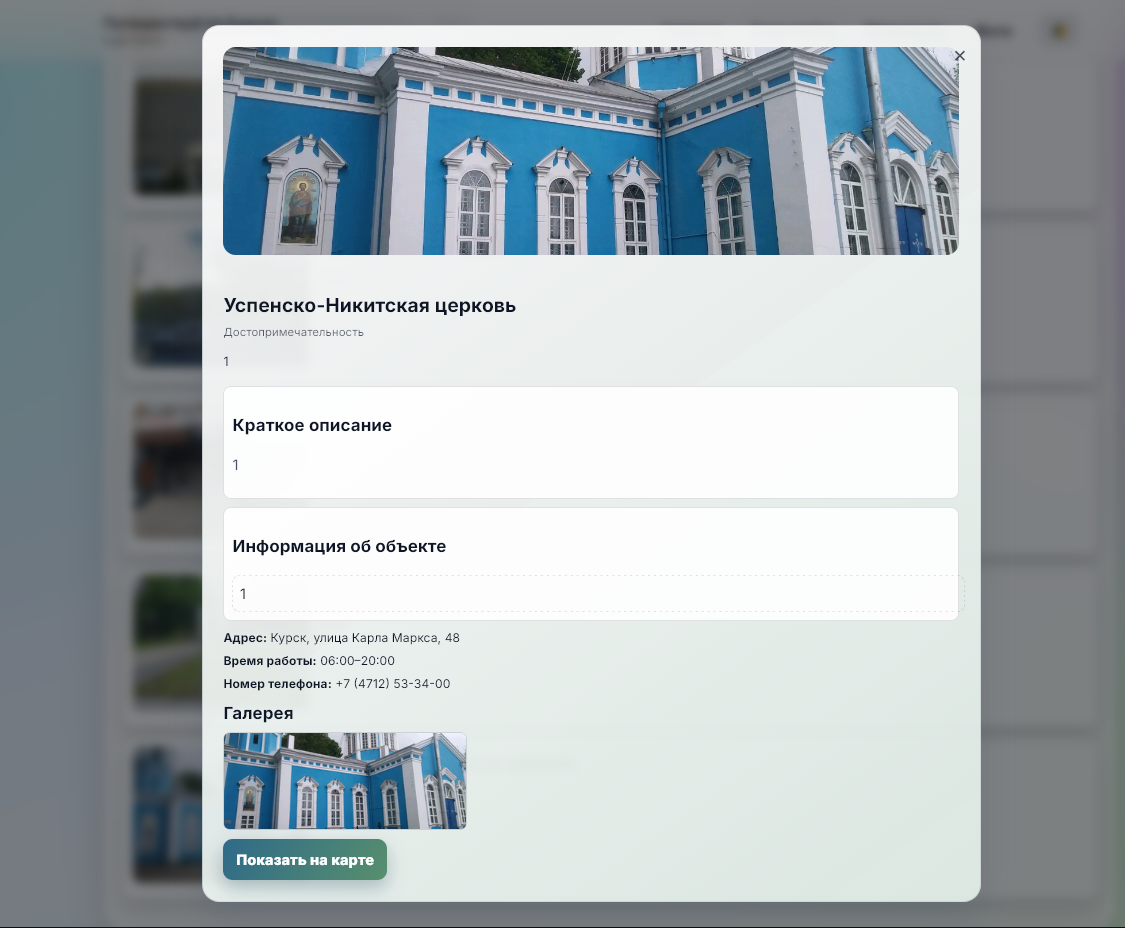
\includegraphics[width=0.8\linewidth]{images/ui-modal-object}
	\caption{Окно просмотра подробной информации об объекте}
	\label{fig:ui-modal-object}
\end{figure}

Окно просмотра карточки маршрута показано на рисунке~\ref{fig:ui-modal-route}.

\begin{figure}[H]
	\centering
	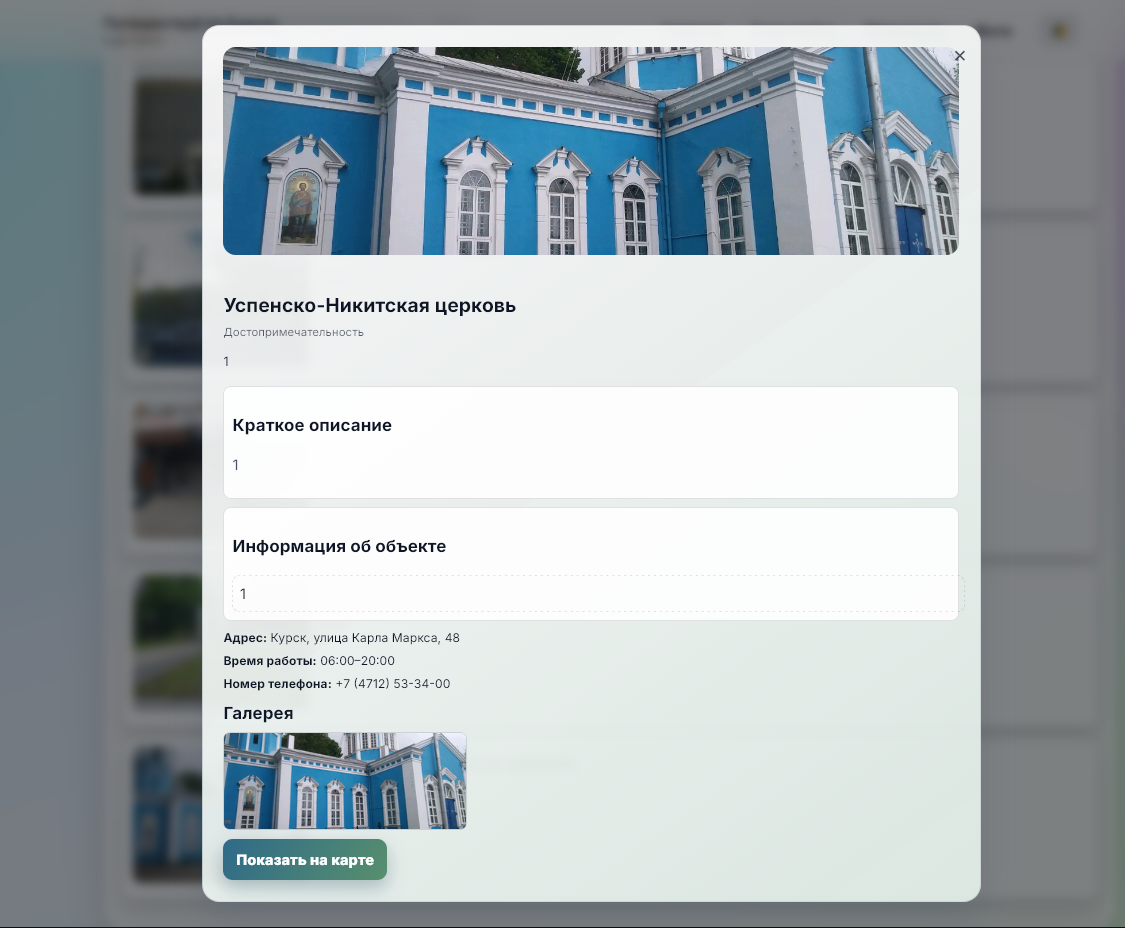
\includegraphics[width=0.8\linewidth]{images/ui-modal-object}
	\caption{Окно просмотра подробной информации о маршруте}
	\label{fig:ui-modal-route}
\end{figure}

\subsection{Моделирование вариантов использования}
В системе выделяются два действующих лица:
\begin{enumerate}
	\item Пользователь --- просматривает опубликованный контент.
	\item Администратор --- управляет контентом системы.
\end{enumerate}

Далее приведены агрегированные перечни прецедентов для каждой роли; они детализируются в последующих подпунктах.

Перечень прецедентов пользователя:
\begin{enumerate}
	\item Просмотреть главную страницу.
	\item Просмотреть карту с маркерами.
	\item Просмотреть список мест.
	\item Отфильтровать места по категории.
	\item Открыть карточку места.
	\item Перейти к месту на карте.
	\item Просмотреть список маршрутов.
	\item Открыть карточку маршрута.
	\item Просмотреть фото-галерею.
	\item Открыть фото в модальном окне.
	\item Открыть связанное место из фото.
\end{enumerate}

\begin{figure}[H]
	\centering
	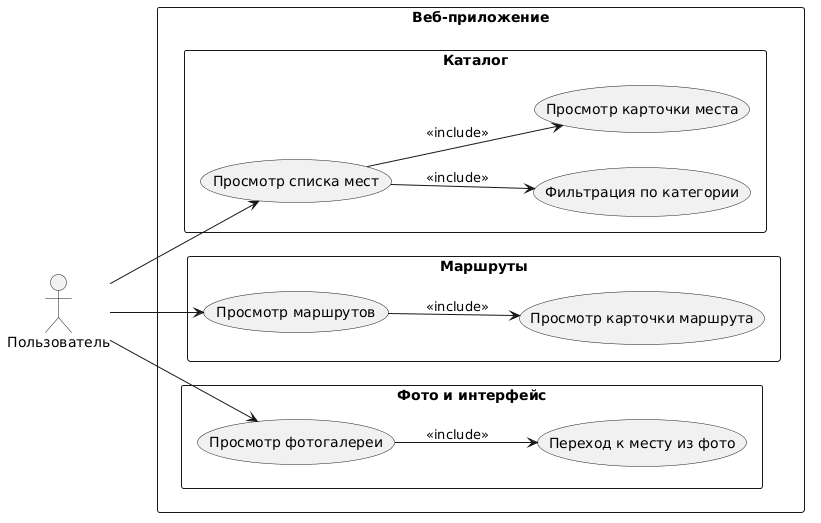
\includegraphics[width=0.8\linewidth]{images/usecase-user}
	\caption{Диаграмма прецедентов для пользователя}
	\label{fig:usecase-user}
\end{figure}

Перечень прецедентов администратора:
\begin{enumerate}
	\item Добавить категорию.
	\item Добавить объект.
	\item Редактировать объект.
	\item Удалить объект.
	\item Опубликовать/скрыть объект.
	\item Выбрать координаты объекта на карте.
	\item Просмотреть список объектов.
	\item Добавить маршрут.
	\item Редактировать маршрут.
	\item Удалить маршрут.
	\item Добавить/удалить/переставить точки маршрута.
	\item Опубликовать/скрыть маршрут.
	\item Просмотреть список маршрутов.
\end{enumerate}

\begin{figure}[H]
	\centering
	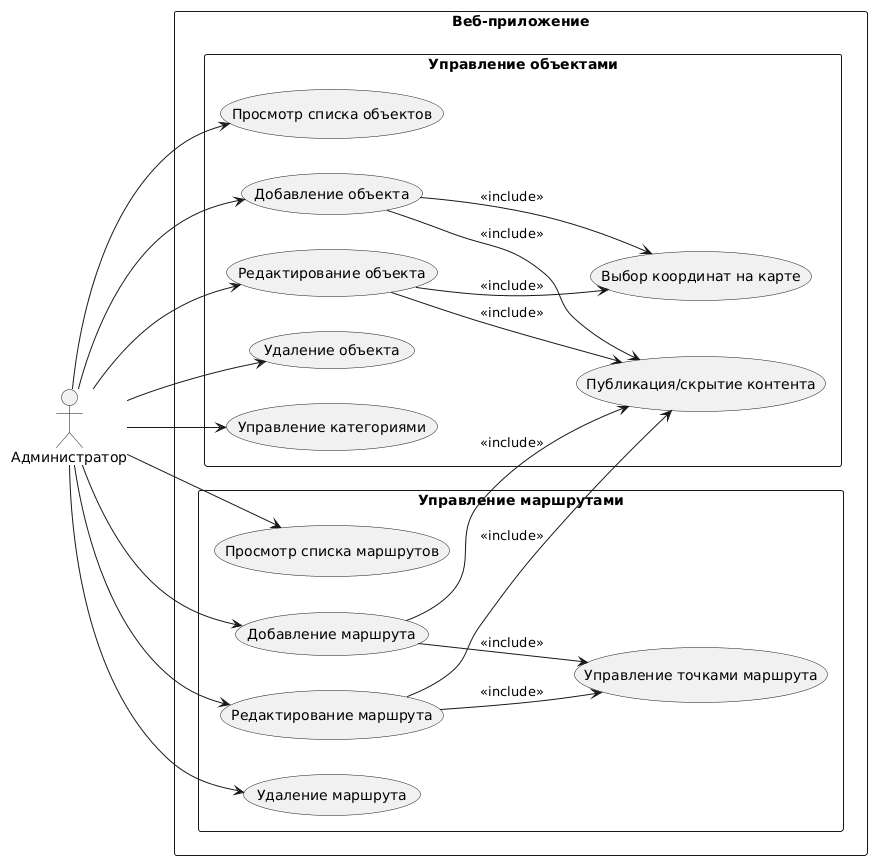
\includegraphics[width=0.8\linewidth]{images/usecase-admin}
	\caption{Диаграмма прецедентов использования для администратора}
	\label{fig:usecase-admin}
\end{figure}

\subsubsection{Вариант использования «Просмотр списка мест»}
\textbf{Заинтересованные лица и их требования:} пользователь желает увидеть доступные места города.

\textbf{Предусловие:} открыта страница «Куда пойти».

\textbf{Постусловие:} отображён список опубликованных объектов.

\textbf{Основной успешный сценарий:}
\begin{enumerate}
	\item Пользователь открывает страницу «Куда пойти».
	\item Система запрашивает категории и опубликованные места через API.
	\item Система формирует карточки мест.
	\item Пользователь просматривает список.
\end{enumerate}

\subsubsection{Вариант использования «Фильтрация мест по категории»}
\textbf{Заинтересованные лица и их требования:} пользователь желает быстро отобрать места по интересующей категории.

\textbf{Предусловие:} список мест загружен, доступны кнопки/элементы фильтрации по категориям.

\textbf{Постусловие:} отображаются только места выбранной категории.

\textbf{Основной успешный сценарий:}
\begin{enumerate}
	\item Пользователь выбирает категорию.
	\item Система применяет фильтр к текущему набору мест.
	\item Карточки в списке обновляются.
\end{enumerate}

\textbf{Альтернативный сценарий (пустой результат):}
\begin{enumerate}
	\item В желаемой категории отсутствуют места.
	\item Система не даёт возможность выбрать категорию.
\end{enumerate}

\subsubsection{Вариант использования «Просмотр карточки места»}
\textbf{Заинтересованные лица и их требования:} пользователь желает получить подробную информацию о конкретном месте.

\textbf{Предусловие:} место отображается в списке или на карте.

\textbf{Постусловие:} открыто модальное окно с детальной информацией о месте.

\textbf{Основной успешный сценарий:}
\begin{enumerate}
	\item Пользователь выбирает карточку места (или маркер на карте).
	\item Система открывает модальное окно.
	\item Отображаются название, описание, контакты, адрес, галерея и ссылки.
\end{enumerate}

\textbf{Альтернативный сценарий (неполные данные):}
\begin{enumerate}
	\item У места отсутствуют часть полей (например, сайт/телефон).
	\item Система скрывает или оставляет пустыми отсутствующие поля.
\end{enumerate}

\subsubsection{Вариант использования «Просмотр мест на карте»}
\textbf{Заинтересованные лица и их требования:} пользователь желает видеть пространственное расположение мест.

\textbf{Предусловие:} открыта главная страница, карта загружена.

\textbf{Постусловие:} пользователь видит маркеры мест и может с ними взаимодействовать.

\textbf{Основной успешный сценарий:}
\begin{enumerate}
	\item Пользователь переходит к блоку карты.
	\item Система отображает карту и маркеры опубликованных мест.
	\item Пользователь кликает по маркеру.
	\item Система открывает карточку соответствующего места.
\end{enumerate}

\subsubsection{Вариант использования «Просмотр списка маршрутов»}
\textbf{Заинтересованные лица и их требования:} пользователь желает получить готовые маршруты прогулок.

\textbf{Предусловие:} открыта страница «Маршруты».

\textbf{Постусловие:} отображён список опубликованных маршрутов.

\textbf{Основной успешный сценарий:}
\begin{enumerate}
	\item Пользователь открывает страницу «Маршруты».
	\item Система запрашивает список маршрутов через API.
	\item Система выводит маршруты в интерфейсе.
\end{enumerate}

\textbf{Альтернативный сценарий (маршрутов нет):} 
\begin{enumerate}
	\item В базе отсутствуют опубликованные маршруты.
	\item Система отображает пустой список.
\end{enumerate}

\subsubsection{Вариант использования «Просмотр карточки маршрута»}
\textbf{Заинтересованные лица и их требования:} пользователь желает получить подробный состав маршрута.

\textbf{Предусловие:} маршрут присутствует в списке.

\textbf{Постусловие:} открыто окно маршрута со списком точек и картой.

\textbf{Основной успешный сценарий:}
\begin{enumerate}
	\item Пользователь выбирает маршрут.
	\item Система открывает модальное окно маршрута.
	\item Отображаются описание и точки маршрута.
	\item Маршрут визуализируется на карте.
\end{enumerate}

\subsubsection{Вариант использования «Просмотр фотогалереи»}
\textbf{Заинтересованные лица и их требования:} пользователь желает просмотреть фото мест города.

\textbf{Предусловие:} открыта страница «Фото».

\textbf{Постусловие:} отображена сетка изображений.

\textbf{Основной успешный сценарий:}
\begin{enumerate}
	\item Пользователь открывает страницу «Фото».
	\item Система формирует галерею из доступных изображений.
	\item Пользователь просматривает сетку фото.
\end{enumerate}

\subsubsection{Вариант использования «Открытие фото в модальном окне»}
\textbf{Заинтересованные лица и их требования:} пользователь желает рассмотреть фото в увеличенном виде.

\textbf{Предусловие:} фото отображается в галерее.

\textbf{Постусловие:} открыто модальное окно с увеличенным изображением.

\textbf{Основной успешный сценарий:}
\begin{enumerate}
	\item Пользователь нажимает на фото.
	\item Система открывает модальное окно.
	\item Отображаются увеличенное фото и действия для дальнейшего перехода.
\end{enumerate}

\subsubsection{Вариант использования «Переход к месту из фото»}
\textbf{Заинтересованные лица и их требования:} пользователь желает перейти от фото к карточке конкретного места.

\textbf{Предусловие:} открыто модальное окно фото.

\textbf{Постусловие:} открыта карточка связанного места.

\textbf{Основной успешный сценарий:}
\begin{enumerate}
	\item Пользователь нажимает кнопку «Что это за место?».
	\item Система определяет связанный объект.
	\item Система открывает карточку места.
\end{enumerate}

\subsubsection{Вариант использования «Вход в панель администратора»}
\textbf{Заинтересованные лица и их требования:} администратор желает получить доступ к функциям управления контентом.

\textbf{Предусловие:} открыта страница администрирования, доступ к панели не подтверждён.

\textbf{Постусловие:} администратор получает доступ к функциям управления объектами и маршрутами.

\textbf{Основной успешный сценарий:}
\begin{enumerate}
	\item Администратор открывает страницу панели.
	\item Система запрашивает подтверждение доступа.
	\item Администратор вводит учётные данные.
	\item Доступ подтверждается.
	\item Отображается интерфейс управления объектами и маршрутами.
\end{enumerate}

\textbf{Альтернативный сценарий (неверные данные доступа):} 
\begin{enumerate}
	\item Администратор вводит неверные данные.
	\item Система отображает отказ в доступе.
	\item Страница управления не открывается.
\end{enumerate}

\subsubsection{Вариант использования «Добавление категории»}
\textbf{Заинтересованные лица и их требования:} администратор желает расширить классификацию объектов.

\textbf{Предусловие:} открыта панель администратора.

\textbf{Постусловие:} новая категория сохранена и доступна в выпадающих списках.

\textbf{Основной успешный сценарий:}
\begin{enumerate}
	\item Администратор вводит название новой категории.
	\item Нажимает кнопку добавления категории.
	\item Система сохраняет категорию в базе данных.
	\item Система обновляет список категорий в форме объекта.
\end{enumerate}

\textbf{Альтернативный сценарий (пустое значение):}
\begin{enumerate}
	\item Администратор оставляет поле категории пустым.
	\item Сохранение не выполняется.
\end{enumerate}

\subsubsection{Вариант использования «Добавление объекта»}
\textbf{Заинтересованные лица и их требования:} администратор желает создать новую карточку места.

\textbf{Предусловие:} открыта панель администратора, загружены категории.

\textbf{Постусловие:} объект сохранён в базе и отображается в списке объектов.

\textbf{Основной успешный сценарий:}
\begin{enumerate}
	\item Администратор заполняет форму объекта.
	\item Нажимает «Сохранить объект».
	\item Система валидирует поля.
	\item Система отправляет данные в API и сохраняет объект.
	\item Список объектов обновляется.
\end{enumerate}

\textbf{Альтернативный сценарий (ошибка валидации):} 
\begin{enumerate}
	\item Обнаружены некорректные или пустые обязательные поля.
	\item Система выводит список ошибок.
	\item Объект не сохраняется.
\end{enumerate}

\subsubsection{Вариант использования «Редактирование объекта»}
\textbf{Заинтересованные лица и их требования:} администратор желает обновить данные существующего объекта.

\textbf{Предусловие:} объект присутствует в списке панели администратора.

\textbf{Постусловие:} обновлённые данные сохранены в базе.

\textbf{Основной успешный сценарий:}
\begin{enumerate}
	\item Администратор нажимает «Редактировать» для выбранного объекта.
	\item Система подставляет текущие данные в форму.
	\item Администратор меняет значения и сохраняет изменения.
	\item Система обновляет объект в базе данных.
\end{enumerate}

\subsubsection{Вариант использования «Удаление объекта»}
\textbf{Заинтересованные лица и их требования:} администратор желает удалить неактуальный объект.

\textbf{Предусловие:} объект существует в базе данных.

\textbf{Постусловие:} объект удалён, список объектов обновлён.

\textbf{Основной успешный сценарий:}
\begin{enumerate}
	\item Администратор выбирает действие «Удалить».
	\item Система выполняет запрос удаления.
	\item Объект удаляется из базы.
	\item Система обновляет список объектов.
\end{enumerate}

\subsubsection{Вариант использования «Выбор координат объекта на карте»}
\textbf{Заинтересованные лица и их требования:} администратор желает точно указать координаты объекта.

\textbf{Предусловие:} открыта форма объекта в панели администратора.

\textbf{Постусловие:} поля широты и долготы заполнены выбранными координатами.

\textbf{Основной успешный сценарий:}
\begin{enumerate}
	\item Администратор открывает модальное окно выбора координат.
	\item Система загружает карту.
	\item Администратор кликает по карте.
	\item Система показывает подтверждение подстановки координат.
	\item После подтверждения координаты переносятся в форму.
\end{enumerate}

\subsubsection{Вариант использования «Добавление маршрута»}
\textbf{Заинтересованные лица и их требования:} администратор желает создать новый маршрут.

\textbf{Предусловие:} в системе есть доступные объекты для выбора точек маршрута.

\textbf{Постусловие:} маршрут сохранён и отображается в списке маршрутов.

\textbf{Основной успешный сценарий:}
\begin{enumerate}
	\item Администратор заполняет название и описание маршрута.
	\item Добавляет минимум две точки маршрута.
	\item Нажимает «Сохранить маршрут».
	\item Система валидирует структуру маршрута.
	\item Система сохраняет маршрут и связанные точки.
\end{enumerate}

\textbf{Альтернативный сценарий (меньше двух точек):} 
\begin{enumerate}
	\item Администратор пытается сохранить маршрут с одной или нулём точек.
	\item Система выводит ошибку валидации.
	\item Маршрут не сохраняется.
\end{enumerate}

\subsubsection{Вариант использования «Редактирование маршрута»}
\textbf{Заинтересованные лица и их требования:} администратор желает изменить параметры существующего маршрута.

\textbf{Предусловие:} маршрут существует в базе данных.

\textbf{Постусловие:} изменения маршрута сохранены.

\textbf{Основной успешный сценарий:}
\begin{enumerate}
	\item Администратор выбирает маршрут в списке.
	\item Система загружает данные маршрута в форму.
	\item Администратор изменяет описание, видимость или точки.
	\item Сохраняет изменения.
	\item Система обновляет маршрут.
\end{enumerate}

\subsubsection{Вариант использования «Удаление маршрута»}
\textbf{Заинтересованные лица и их требования:} администратор желает удалить неактуальный маршрут.

\textbf{Предусловие:} маршрут присутствует в списке маршрутов.

\textbf{Постусловие:} маршрут удалён из базы данных.

\textbf{Основной успешный сценарий:}
\begin{enumerate}
	\item Администратор нажимает «Удалить маршрут».
	\item Система отправляет запрос на удаление.
	\item Маршрут удаляется.
	\item Список маршрутов обновляется.
\end{enumerate}

\subsubsection{Вариант использования «Управление точками маршрута»}
\textbf{Заинтересованные лица и их требования:} администратор желает настроить последовательность прохождения маршрута.

\textbf{Предусловие:} открыта форма добавления/редактирования маршрута.

\textbf{Постусловие:} точки маршрута сохранены в актуальном порядке.

\textbf{Основной успешный сценарий:}
\begin{enumerate}
	\item Администратор добавляет точки из списка доступных объектов.
	\item При необходимости удаляет лишние точки.
	\item Меняет порядок точек кнопками «вверх/вниз».
	\item Система визуально обновляет последовательность.
	\item При сохранении маршрута порядок записывается в базу данных.
\end{enumerate}

\subsubsection{Вариант использования «Управление публикацией контента»}
\textbf{Заинтересованные лица и их требования:} администратор желает контролировать видимость объектов и маршрутов в пользовательской части.

\textbf{Предусловие:} открыт режим редактирования объекта или маршрута.

\textbf{Постусловие:} признак видимости (published/hidden) сохранён.

\textbf{Основной успешный сценарий:}
\begin{enumerate}
	\item Администратор устанавливает/снимает флаг публикации.
	\item Сохраняет изменения.
	\item Система обновляет запись в базе.
	\item Контент появляется или скрывается в пользовательских разделах.
\end{enumerate}

\subsection{Требования к надёжности}
Система должна обеспечивать надёжную обработку и хранение данных как при
обычной эксплуатации, так и при возникновении ошибок.

\textbf{Целостность данных.} Операции создания и обновления маршрутов
выполняются в транзакциях PostgreSQL, что исключает сохранение частично
заполненных маршрутов (например, при ошибке между сохранением маршрута и
сохранением его точек).

\textbf{Устойчивость API.} Серверная часть должна корректно обрабатывать
ошибки и возвращать стандартизированные ответы JSON с кодами HTTP 4xx/5xx
без аварийного завершения процесса Node.js.

\textbf{Валидация входных данных.} На стороне клиентского административного
интерфейса и на стороне API должна выполняться проверка обязательных полей
(название, категория, координаты, структура маршрута), чтобы предотвратить
попадание некорректных записей в базу данных.

\textbf{Логирование ошибок.} Ошибки API должны фиксироваться в журнале
приложения (stdout/stderr или файл логов окружения), включая текст ошибки и
контекст запроса для последующей диагностики.

\textbf{Резервное копирование.} Для обеспечения сохранности данных должно
выполняться регулярное резервное копирование базы PostgreSQL штатными
средствами (pg\_dump/pg\_restore) или средствами инфраструктуры.

\subsection{Требования к информационной безопасности}
Система должна обеспечивать защиту данных и административного контура от
несанкционированного доступа.

\textbf{Разграничение доступа к админ-разделу.} Доступ к
странице \texttt{/pages/admin.html} должен ограничиваться на уровне
инфраструктуры.

\textbf{Защита от SQL-инъекций.} Все обращения к базе данных должны
выполняться через параметризованные SQL-запросы.

\textbf{Валидация пользовательского ввода.} Все текстовые и URL-поля,
передаваемые через API, должны проверяться на корректность формата и длины
для предотвращения передачи вредоносных или некорректных данных.

\textbf{Защита административных операций.} Действия удаления и публикации
контента должны выполняться только через административный интерфейс и
журналироваться средствами сервера/инфраструктуры.

\subsection{Требования к программной и технической совместимости}
Система должна корректно функционировать в типовой среде разработки и
развёртывания веб-приложений.

\textbf{Операционная система сервера.} Серверная часть должна работать в
средах Linux, Windows и macOS при наличии Node.js и PostgreSQL совместимых
версий.

\textbf{Программные зависимости.} Для работы приложения необходимы:
Node.js, пакетный менеджер npm, СУБД PostgreSQL, а также доступ к внешнему
скрипту Yandex Maps API.

\textbf{Требования к браузеру.} Клиентская часть должна корректно
отображаться в актуальных версиях Google Chrome, Mozilla Firefox,
Microsoft Edge и других современных браузерах с поддержкой ES6.

\textbf{Совместимость данных.} Приложение должно работать с БД PostgreSQL,
содержащей таблицы \texttt{categories}, \texttt{places}, \texttt{routes},
\texttt{route\_points}.

\subsection{Требования к оформлению документации}
Разработка программной документации и программного изделия должна производиться согласно ГОСТ 19.102-77 и ГОСТ 34.601-90. Единая система программной документации.

\section{Технический проект}

\subsection{Архитектура программной системы}
Программная система «Цифровая платформа Курский край» реализована по архитектуре «клиент--сервер».
Клиентская часть представлена веб-интерфейсом на HTML/CSS/JavaScript,
который открывается в браузере пользователя. Серверная часть реализована на
Node.js (Express) и предоставляет REST API для чтения и изменения данных.
Хранение данных выполняется в СУБД PostgreSQL.

Выбор такой архитектуры обоснован требованиями проекта: необходимо обеспечить
одновременную работу пользовательской части (просмотр мест, маршрутов, фото)
и административной части (управление объектами и маршрутами) с единой базой
данных. Сервер централизует бизнес-логику, валидацию, а также контроль
доступности опубликованного контента.

Общая схема взаимодействия компонентов приведена на рисунке~\ref{fig:arch-overall}.

\begin{figure}[H]
	\centering
	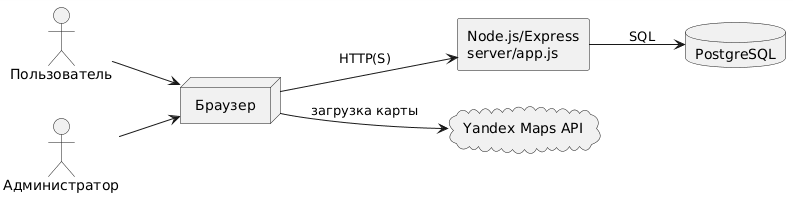
\includegraphics[width=0.85\linewidth, height=4.5cm]{images/arch-overall}
	\caption{Общая схема взаимодействия компонентов}
	\label{fig:arch-overall}
\end{figure}

Серверное приложение обрабатывает HTTP-запросы, маршрутизирует их по эндпоинтам
\texttt{/api/categories}, \texttt{/api/places}, \texttt{/api/routes}, выполняет SQL-запросы к PostgreSQL и
возвращает клиенту данные в формате JSON. Статические страницы пользовательского
и административного интерфейса раздаются тем же Node.js-приложением.

\subsection{Обоснование выбора технологий проектирования}
При выборе технологического стека учитывались требования простоты запуска,
поддерживаемости, возможности работы с картографическими данными и
транзакционного хранения сведений о местах и маршрутах. Выбранный стек
состоит из Node.js/Express на сервере, чистого JavaScript на клиенте,
PostgreSQL в качестве СУБД и Yandex Maps API для отображения карт.

\subsubsection{JavaScript (Node.js) как серверная платформа}
Использование Node.js обосновано тем, что проект использует единый язык
(JavaScript) на клиенте и сервере, что упрощает сопровождение и снижает
порог входа при доработках. Асинхронная модель Node.js подходит для
обработки множества параллельных HTTP-запросов.

Node.js/Express обеспечивает быстрый старт разработки, прозрачную маршрутизацию
и единый язык на фронтенде и бэкенде. Это сокращает стоимость сопровождения и
ускоряет внедрение изменений.

При этом у выбранного стека есть инженерные ограничения:
\begin{enumerate}
	\item Однопоточная event-loop модель чувствительна к блокирующим CPU-операциям.
	\item Типизация JavaScript по умолчанию слабее строготипизированных языков.
	\item Рост проекта требует дополнительной дисциплины архитектурных границ
	(слои, контракты, тесты), иначе возрастает риск «разрастания» контроллеров.
\end{enumerate}

В рамках текущего проекта эти недостатки компенсируются:
\begin{itemize}
	\item выносом тяжёлой логики в SQL и транзакции БД;
	\item модульной структурой клиентского и серверного кода;
	\item строгими API-контрактами и единообразной обработкой ошибок.
\end{itemize}

\subsubsection{Express как веб-фреймворк}
Express выбран как минималистичный и расширяемый фреймворк,
предоставляющий:
\begin{itemize}
	\item маршрутизацию HTTP-запросов;
	\item middleware-подход для обработки JSON и ошибок;
	\item удобную интеграцию с раздачей статических файлов.
\end{itemize}

\subsubsection{PostgreSQL как СУБД}
PostgreSQL обеспечивает транзакционность, ограничения целостности,
надёжную работу с внешними ключами и удобные средства агрегации данных,
которые используются при формировании структур маршрутов с точками.

PostgreSQL выбран как промышленная СУБД с развитой поддержкой транзакций,
ограничений целостности и JSON-операций. Для проекта, где одновременно используются
структурированные сущности (места/маршруты) и вложенные коллекции (галерея,
агрегированные точки маршрута), такой баланс особенно важен.

Альтернативы и их ограничения для данного контекста:
\begin{enumerate}
	\item SQLite: простота развёртывания, но ограниченная модель конкурентной записи
	при интенсивной административной работе.
	\item MySQL/MariaDB: сопоставимая функциональность, но потребовалась бы отдельная
	адаптация SQL-диалекта и миграций под уже выбранный стек.
	\item NoSQL-подход: удобен для документов, но усложняет строгую целостность
	связей маршрутов и мест при требованиях предсказуемой реляционной модели.
\end{enumerate}

Следовательно, PostgreSQL является технически обоснованным компромиссом между
надёжностью, выразительностью запросов и устойчивостью к росту проекта.

\subsubsection{Vanilla JavaScript на клиенте}
Клиентская часть реализована без тяжёлых frontend-фреймворков.
Это снижает сложность сборки, упрощает развёртывание и хорошо подходит
для проекта с акцентом на справочный интерфейс и CRUD-операции.

Отказ от крупного frontend-фреймворка снижает порог сопровождения и убирает
сложность build-пайплайна. Для проекта с умеренной интерактивностью это
рационально: критическая ценность лежит в контенте и карте, а не в сложной
реактивной UI-модели.

Ограничения такого выбора:
\begin{itemize}
	\item при масштабировании интерфейса возрастает объём ручного управления состоянием;
	\item выше риск дублирования DOM-логики между страницами;
	\item сложнее унифицировать паттерны жизненного цикла компонентов.
\end{itemize}

В техническом проекте эти риски адресуются через модульную декомпозицию
(страничные модули и общий слой \texttt{places-store.js} и API-обёртки).

\subsubsection{Интеграция с Yandex Maps API}
Для картографической функциональности использован Yandex Maps API,
что позволяет:
\begin{itemize}
	\item отображать объекты на карте;
	\item выбирать координаты в административном интерфейсе;
	\item визуализировать маршруты в пользовательской части.
\end{itemize}

Использование готового картографического API уменьшает объём собственной
разработки и позволяет сосредоточиться на предметной логике проекта: хранении
объектов, управлении маршрутами и отображении туристического контента.

\subsection{Клиентская часть}
Структура клиентского слоя включает HTML-страницы и
набор JS-модулей, каждый из которых отвечает за свой сценарий работы.

Назначение HTML-страниц определяется следующим образом:
\begin{enumerate}
	\item Страница \texttt{index.html} является входной точкой пользовательского интерфейса и содержит обзорный экран проекта.
	\item Страница \texttt{places.html} предназначена для просмотра каталога мест, фильтрации по категориям и открытия карточек объектов.
	\item Страница \texttt{routes.html} используется для отображения маршрутов, состава точек маршрута и связанных объектов.
	\item Страница \texttt{photos.html} реализует фотогалерею и переходы к карточкам мест по выбранным изображениям.
	\item Страница \texttt{admin.html} предназначена для административных операций: создания, редактирования и удаления категорий, объектов и маршрутов.
\end{enumerate}

Назначение основных JavaScript-файлов следующее:
\begin{enumerate}
	\item Модуль \texttt{places-page.js} загружает данные каталога мест через API, применяет фильтры и управляет визуализацией карточек.
	\item Модуль \texttt{routes-page.js} запрашивает маршруты, строит структуру точек и отображает связанный маршрутный контент.
	\item Модуль \texttt{photos-page.js} подготавливает данные галереи и обрабатывает переходы пользователя между фото и карточками объектов.
	\item Модуль \texttt{admin-page.js} реализует формы CRUD-операций, валидацию перед отправкой и синхронизацию таблиц после изменений.
	\item Модуль \texttt{api\_places.js} инкапсулирует HTTP-вызовы к серверным endpoint-ам и унифицирует обработку ответов.
	\item Модуль \texttt{places-store.js} хранит клиентское состояние каталога и промежуточные структуры для фильтрации.
	\item Модуль \texttt{theme.js} отвечает за переключение темы и сохранение пользовательских настроек отображения.
\end{enumerate}

Диаграмма компонентов клиентской части приведена на рисунке~\ref{fig:arch-client}.

\begin{figure}[H]
	\centering
	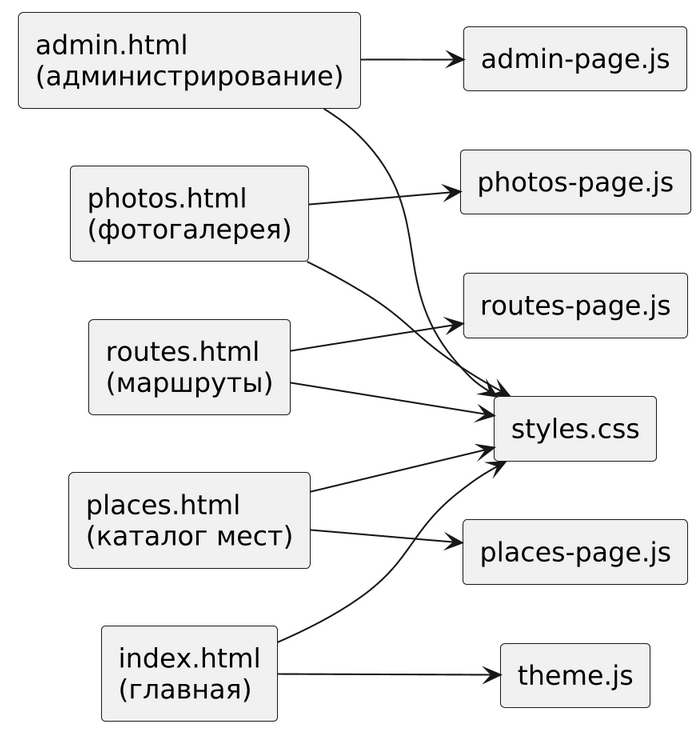
\includegraphics[width=0.5\linewidth, height=10cm]{images/arch-client}
	\caption{Диаграмма компонентов клиентской части}
	\label{fig:arch-client}
\end{figure}

Навигационная структура состоит из четырёх пользовательских страниц и одной
административной. Во всех страницах применяется единый заголовок,
меню навигации и механизм переключения темы, что снижает когнитивную
нагрузку и обеспечивает консистентность UX.

Модули клиентской части разделены по принципу «страница/домен»:
\begin{enumerate}
	\item \texttt{places-page.js} --- каталог мест и модальные карточки.
	\item \texttt{routes-page.js} --- маршруты и визуализация маршрута.
	\item \texttt{photos-page.js} --- галерея и переход к связанным местам.
	\item \texttt{admin-page.js} --- CRUD для объектов и маршрутов.
	\item \texttt{places-store.js} --- общий слой нормализации и валидации на клиенте.
	\item \texttt{api\_places.js} --- HTTP-взаимодействие с API.
	\item \texttt{theme.js} --- управление темой интерфейса.
\end{enumerate}

Такое разделение снижает связность, упрощает модульное сопровождение и
позволяет локально дорабатывать функциональность без каскадных изменений
в других частях фронтенда.

\subsection{Серверная часть}
Серверная часть реализована в модуле \texttt{server/app.js}. Центральный компонент
--- Express-приложение, выполняющее следующие функции:
\begin{itemize}
	\item обслуживание REST API для сущностей \texttt{categories}, \texttt{places}, \texttt{routes};
	\item валидация обязательных параметров в запросах создания/изменения;
	\item формирование агрегированных структур маршрутов (с точками и данными мест);
	\item обработка ошибок и возврат стандартизированных JSON-ответов;
	\item раздача статических файлов клиентской части.
\end{itemize}

Модуль \texttt{server/db.js} инкапсулирует подключение к PostgreSQL. Модуль
\texttt{server/init-db.js} отвечает за первичное развёртывание структуры БД и
инициализацию справочников.

Диаграмма компонентов серверной части приведена на рисунке~\ref{fig:arch-server}.

\begin{figure}[H]
	\centering
	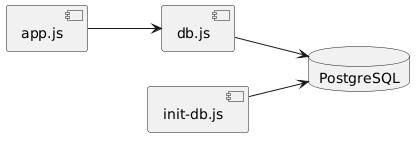
\includegraphics[width=0.8\linewidth]{images/arch-server}
	\caption{Диаграмма компонентов серверной части}
	\label{fig:arch-server}
\end{figure}

\subsubsection{Маршруты}

Маршруты API имеют общий префикс \texttt{/api}. Для административных сценариев
чтения используется query-параметр \texttt{includeHidden=1}, позволяющий получить
как опубликованные, так и скрытые записи. Основные HTTP-запросы серверной части
представлены в таблице \ref{tab:api-http}.
\begin{xltabular}{\textwidth}{|c|l|l|X|}
	\caption{Основные HTTP-запросы}
	\label{tab:api-http}
	\finishhead
	\hline
	Маршрут & Метод & Входные данные & Результат \\ \hline
	\texttt{/api/categories} & GET & --- & JSON-массив категорий \\ \hline
	\texttt{/api/categories} & POST & JSON-тело категории & Создание или обновление категории; при ошибке возвращается JSON с полем \texttt{error} \\ \hline
	\texttt{/api/places} & GET & Query-параметр & JSON-массив опубликованных мест или полный список при \texttt{includeHidden=1} \\ \hline
	\texttt{/api/places} & POST & JSON-тело места & Создание или обновление места; при ошибке возвращается JSON с полем \texttt{error} \\ \hline
	\texttt{/api/places/:id} & DELETE & \texttt{id} в URL & Удаление места; при успехе возвращается пустой ответ со статусом \texttt{204} \\ \hline
	\texttt{/api/routes} & GET & Query-параметр & JSON-массив опубликованных маршрутов с точками или полный список при \texttt{includeHidden=1} \\ \hline
	\texttt{/api/routes} & POST & JSON-тело маршрута & Создание или обновление маршрута с точками; при ошибке возвращается JSON с полем \texttt{error} \\ \hline
	\texttt{/api/routes/:id} & DELETE & \texttt{id} в URL & Удаление маршрута; при успехе возвращается пустой ответ со статусом \texttt{204} \\ \hline
\end{xltabular}

Пример успешного ответа \texttt{GET /api/categories}:
\begin{verbatim}
	[
	{
		"slug": "parks",
		"label": "Парки"
	}
	]
\end{verbatim}

Пример успешного ответа \texttt{POST /api/categories}:
\begin{verbatim}
	{
		"slug": "museums",
		"label": "Музеи"
	}
\end{verbatim}

Возможное сообщение об ошибке для \texttt{POST /api/categories}:
\begin{verbatim}
	{
		"error": "slug and label are required"
	}
\end{verbatim}

Пример успешного ответа \texttt{GET /api/places} и
\texttt{GET /api/places?includeHidden=1}:
\begin{verbatim}
	[
	{
		"id": "krasnaya-ploshchad",
		"name": "Красная площадь",
		"category": "attractions",
		"description": "Центральная площадь Курска",
		"object_info": "Исторический центр города",
		"lat": "51.730100",
		"lon": "36.193900",
		"cover_image_url": "image.com",
		"gallery": ["images/krasnaya.jpg"],
		"address": "г. Курск, Красная площадь",
		"open_hours": "Круглосуточно",
		"phone": "",
		"website_url": "",
		"visible": true,
		"updated_at": "2026-05-07T10:00:00.000Z"
	}
	]
\end{verbatim}

Пример успешного ответа \texttt{POST /api/places}:
\begin{verbatim}
	{
		"id": "krasnaya-ploshchad",
		"name": "Красная площадь",
		"category": "attractions",
		"description": "Центральная площадь Курска",
		"object_info": "Исторический центр города",
		"lat": "51.730100",
		"lon": "36.193900",
		"cover_image_url": "image.com",
		"gallery": ["images/krasnaya.jpg"],
		"address": "г. Курск, Красная площадь",
		"open_hours": "Круглосуточно",
		"phone": "",
		"website_url": "",
		"visible": true,
		"updated_at": "2026-05-07T10:00:00.000Z"
	}
\end{verbatim}

Для \texttt{DELETE /api/places/:id} при успешном выполнении сервер возвращает
статус \texttt{204 No Content}; JSON-тело ответа отсутствует.

Пример успешного ответа \texttt{GET /api/routes} и
\texttt{GET /api/routes?includeHidden=1}:
\begin{verbatim}
	[
	{
		"id": "historic-center",
		"name": "Исторический центр",
		"short_description": "Пешеходный маршрут по центру Курска",
		"description": "Маршрут объединяет ключевые городские достопримечательности.",
		"visible": true,
		"updated_at": "2026-05-07T10:00:00.000Z",
		"points": [
		{
			"place_id": "krasnaya-ploshchad",
			"position": 0,
			"place_name": "Красная площадь",
			"lat": "51.730100",
			"lon": "36.193900",
			"cover_image_url": "image.com",
			"category": "attractions"
		}
		]
	}
	]
\end{verbatim}

Пример успешного ответа \texttt{POST /api/routes}:
\begin{verbatim}
	{
		"id": "historic-center",
		"name": "Исторический центр",
		"short_description": "Пешеходный маршрут по центру Курска",
		"description": "Маршрут объединяет ключевые городские достопримечательности.",
		"visible": true,
		"updated_at": "2026-05-07T10:00:00.000Z",
		"points": [
		{
			"place_id": "krasnaya-ploshchad",
			"position": 0,
			"place_name": "Красная площадь",
			"lat": "51.730100",
			"lon": "36.193900",
			"cover_image_url": "image.com",
			"category": "attractions"
		},
		{
			"place_id": "znamsobor",
			"position": 1,
			"place_name": "Знаменский собор",
			"lat": "51.730900",
			"lon": "36.191800",
			"cover_image_url": "image.com",
			"category": "religion"
		}
		]
	}
\end{verbatim}

Возможные сообщения об ошибках для \texttt{POST /api/routes}:
\begin{verbatim}
	{
		"error": "Route name is required"
	}
\end{verbatim}

\begin{verbatim}
	{
		"error": "Route must contain at least start and end points"
	}
\end{verbatim}

Для \texttt{DELETE /api/routes/:id} при успешном выполнении сервер возвращает
статус \texttt{204 No Content}; JSON-тело ответа отсутствует.

Общий формат ошибки для обработчиков API:
\begin{verbatim}
	{
		"error": "текст ошибки"
	}
\end{verbatim}

Помимо перечисленных ошибок валидации, сервер может вернуть JSON-ответ со
статусом \texttt{500}, если произошла внутренняя ошибка приложения или ошибка
доступа к базе данных. В этом случае поле \texttt{error} содержит текст ошибки,
полученный обработчиком Express или транзакционным обработчиком сохранения
маршрута.

\subsubsection{Детализация функциональных подсистем}
Подсистема «Каталог мест» обеспечивает основной сценарий ознакомления
пользователя с содержанием платформы. Функционально она включает три слоя:
слой выдачи данных API, слой клиентской фильтрации и слой визуализации карточек.

На серверной стороне запрос \texttt{GET /api/places} возвращает только опубликованные
записи (\texttt{visible = true}), что реализует безопасность представления контента:
черновые или временно скрытые объекты не попадают в публичный интерфейс.
Административный режим использует \texttt{GET /api/places?includeHidden=1},
позволяющий работать с полным набором данных.

На клиентской стороне фильтрация по категориям реализована без повторного запроса
в БД для каждого клика, что уменьшает сетевые задержки. Такой подход рационален
для текущего объёма данных, характерного для городского гида. При дальнейшем росте
набора мест (например, на порядок) возможен переход к серверной фильтрации с
передачей параметров в API.

Подсистема маршрутов решает две взаимосвязанные задачи: хранение структуры
маршрута и визуализация последовательности точек. В техническом проекте это
реализовано через пару сущностей \texttt{routes} и \texttt{route\_points}, где
\texttt{route\_points.position} задаёт порядок прохождения.

Запрос \texttt{GET /api/routes} использует агрегацию точек в JSON-структуру.
Это уменьшает число клиентских запросов и сокращает объём «склейки» данных на
фронтенде. Компромисс такого решения --- более сложный SQL на стороне сервера,
однако выигрыш в целостности и предсказуемости ответа для UI является существенным.

Сохранение маршрута выполняется транзакционно, что особенно важно при операциях
редактирования. Если бы обновление маршрута и точек выполнялось раздельно без
транзакции, при сбое система могла бы получить маршрут без точек либо с частичным
набором точек, что нарушило бы корректность пользовательского сценария.

Административная подсистема включает операции CRUD для категорий, мест и маршрутов.
Ключевым инженерным требованием является устойчивость к невалидному вводу.
Поэтому в проекте предусмотрена двухуровневая валидация:
\begin{enumerate}
	\item Первичная --- на уровне формы и клиентской логики.
	\item Окончательная --- на уровне API перед выполнением SQL-операций.
\end{enumerate}

Серверная валидация обязательна даже при наличии клиентской, поскольку клиентский
код потенциально может быть изменён пользователем. Таким образом, архитектура
ориентирована на модель «не доверять клиенту».

\subsection{Проект базы данных программно-информационной системы}
Проект базы данных описывает логическую модель хранения категорий, объектов,
маршрутов и точек маршрутов. Схема ориентирована на реляционное хранение данных
и поддержку ссылочной целостности между основными сущностями.

\subsubsection{Компоненты базы данных}
Уровень данных построен на PostgreSQL и включает таблицы \texttt{categories},
\texttt{places}, \texttt{routes}, \texttt{route\_points}. Для маршрутов реализована связь
«один-ко-многим»: один маршрут содержит множество точек, каждая точка
ссылается на конкретный объект (place).

При сохранении маршрута операции выполняются в транзакции:
\begin{enumerate}
	\item Создаётся/обновляется запись маршрута.
	\item Удаляются старые точки маршрута.
	\item Вставляется новая последовательность точек.
\end{enumerate}
Это обеспечивает целостность данных и отсутствие «частично сохранённых» маршрутов.

Диаграмма компонентов уровня данных приведена на рисунке~\ref{fig:arch-db}.

\begin{figure}[H]
	\centering
	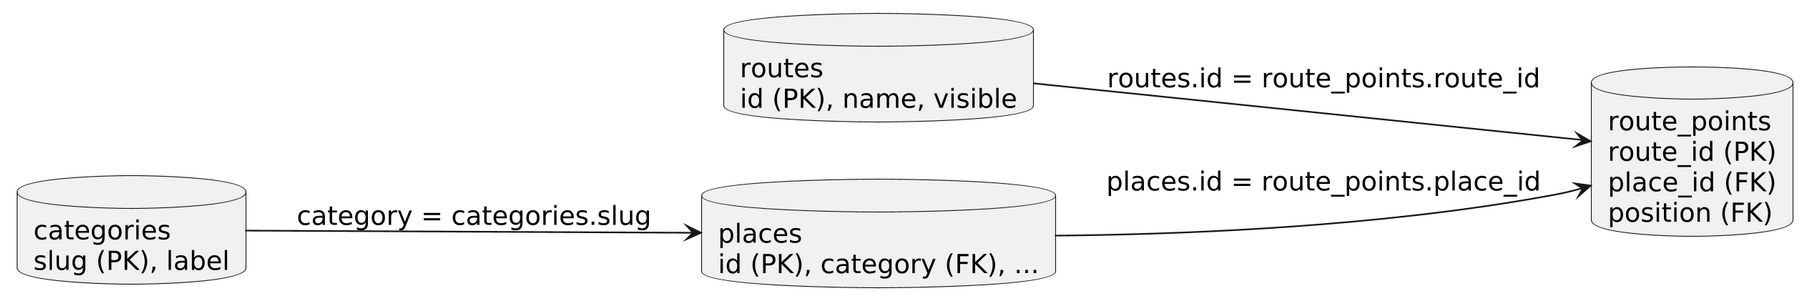
\includegraphics[width=1\linewidth, height=3.5cm]{images/arch-db}
	\caption{Диаграмма компонентов базы данных}
	\label{fig:arch-db}
\end{figure}

\subsubsection{ER-модель данных}
Ключевые сущности базы данных:
\begin{enumerate}
	\item \texttt{categories} --- справочник категорий объектов.
	\item \texttt{places} --- карточки мест (координаты, описания, контакты, видимость).
	\item \texttt{routes} --- маршруты (название, описания, видимость).
	\item \texttt{route\_points} --- точки маршрутов и их порядок.
\end{enumerate}

Связи между сущностями следующие:
\begin{enumerate}
	\item \texttt{categories (1) --- (N) places}.
	\item \texttt{routes (1) --- (N) route\_points}.
	\item \texttt{places (1) --- (N) route\_points}.
\end{enumerate}

ER-диаграмма приведена на рисунке~\ref{fig:db-er}.
\begin{figure}[H]
	\centering
	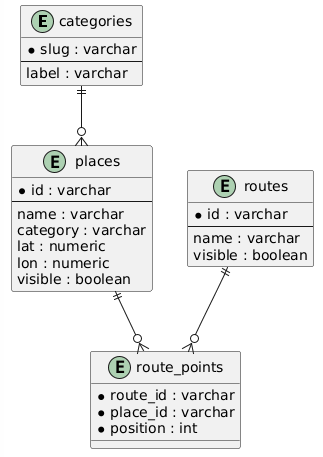
\includegraphics[width=0.45\linewidth, height=10cm]{images/db-er}
	\caption{ER-диаграмма базы данных}
	\label{fig:db-er}
\end{figure}

\subsubsection{Нормализация}
Схема данных приведена к третьей нормальной форме:
\begin{itemize}
	\item справочные значения категорий вынесены в отдельную таблицу;
	\item маршрут и его точки разделены на отдельные сущности;
	\item порядок точек хранится отдельным атрибутом \texttt{position};
	\item отсутствуют повторяющиеся группы атрибутов в одной таблице.
\end{itemize}

Нормализация снижает риск противоречивого хранения данных. Например, категория
объекта хранится в отдельной таблице, а маршрут не содержит повторяющиеся поля
мест: вместо этого используется связующая таблица \texttt{route\_points}.

\subsubsection{Реляционная модель данных}
Реляционная модель включает:
\begin{itemize}
	\item первичные ключи в каждой таблице;
	\item внешние ключи для связей между таблицами;
	\item ограничения уникальности (например, уникальный \texttt{slug} категории);
	\item флаги видимости для публикации/скрытия контента.
\end{itemize}

Для маршрутов используется составной первичный ключ \texttt{(route\_id, position)},
что обеспечивает уникальность позиции точки внутри конкретного маршрута.
Связь с таблицей \texttt{places} не допускает добавления в маршрут несуществующего
объекта.

\subsubsection{Описание структуры таблиц}
В таблицах~\ref{tab:categories}–\ref{tab:route-points} приведено описание структуры таблиц базы данных.
\begin{xltabular}{\textwidth}{|c|c|l|l|X|}
	\caption{Атрибуты таблицы «categories»}
	\label{tab:categories}
	\finishhead
	\hline
	Key Type & Optionality & Column name & Data Type & Size \\ \hline
	PK & * & slug & VARCHAR & 80 \\ \hline
	& * & label & VARCHAR & 200 \\ \hline
\end{xltabular}

\begin{xltabular}{\textwidth}{|c|c|l|l|X|}
	\caption{Атрибуты таблицы «places»}
	\label{tab:places}
	\finishhead
	\hline
	Key Type & Optionality & Column name & Data Type & Size \\ \hline
	PK & * & id & VARCHAR & 80 \\ \hline
	& * & name & VARCHAR & 255 \\ \hline
	& * & category & VARCHAR & 80 \\ \hline
	& * & description & TEXT &  \\ \hline
	&  & object\_info & TEXT & \\ \hline
	&  & lat & NUMERIC & 10,6 \\ \hline
	&  & lon & NUMERIC & 10,6 \\ \hline
	& * & cover\_image\_url & TEXT &  \\ \hline
	& * & gallery & JSONB &  \\ \hline
	&  & address & VARCHAR & 255 \\ \hline
	&  & open\_hours & VARCHAR & 120 \\ \hline
	&  & phone & VARCHAR & 12 \\ \hline
	&  & website\_url & VARCHAR & 255 \\ \hline
	& * & visible & BOOLEAN & \\ \hline
	& * & updated\_at & TIMESTAMPT & yyyy-mm-dd
	hh:mm:ss \\ \hline
\end{xltabular}

\begin{xltabular}{\textwidth}{|c|c|l|l|X|}
	\caption{Атрибуты таблицы «routes»}
	\label{tab:routes}
	\finishhead
	\hline
	Key Type & Optionality & Column name & Data Type & Size \\ \hline
	PK & * & id & VARCHAR & 80 \\ \hline
	& * & name & VARCHAR & 255 \\ \hline
	&   & short\_description & TEXT &  \\ \hline
	&   & description & TEXT &  \\ \hline
	& * & visible & BOOLEAN & \\ \hline
	& * & updated\_at & TIMESTAMPT & yyyy-mm-dd
	hh:mm:s \\ \hline
\end{xltabular}

\begin{xltabular}{\textwidth}{|c|c|l|l|X|}
	\caption{Атрибуты таблицы «route\_points»}
	\label{tab:route-points}
	\finishhead
	\hline
	Key Type & Optionality & Column name & Data Type & Size \\ \hline
	PK & * & route\_id & VARCHAR & 80 \\ \hline
	FK & * & place\_id & VARCHAR & 80 \\ \hline
	FK & * & position & INTEGER &  \\ \hline
\end{xltabular}

\subsubsection{Детализация SQL-запросов и операций доступа к данным}
Запросы чтения разделены на пользовательские и административные профили.
Пользовательский профиль ограничивает выдачу опубликованным контентом, тогда как
административный позволяет видеть все записи. Такое разграничение реализуется
без дублирования таблиц и без усложнения схемы БД.

Для маршрутов применяется \texttt{LEFT JOIN} с таблицей точек и таблицей мест,
что позволяет формировать полный ответ даже в случае частичной неполноты связанных
данных. Дополнительно используется сортировка по \texttt{updated\_at DESC},
обеспечивающая приоритет актуального контента в выдаче.

Операции записи для мест и маршрутов реализованы в стиле \texttt{UPSERT}
(\texttt{INSERT ... ON CONFLICT DO UPDATE}). Это снижает вероятность ошибок при
повторных сохранениях и упрощает клиентскую логику: интерфейсу не требуется
разделять технические ветки «создать» и «обновить» на уровне разных endpoint'ов.

Удаление выполняется через \texttt{DELETE} по идентификатору сущности.
Для маршрутов удаление основной записи приводит к удалению связанных точек
маршрута согласно ограничениям целостности (при настроенном каскаде) либо через
явное удаление в транзакционном блоке.

Основные риски SQL-слоя:
\begin{itemize}
	\item SQL-инъекции при небезопасной конкатенации строк;
	\item «потерянные обновления» при конкурентном редактировании;
	\item рост времени ответа при увеличении объёма данных.
\end{itemize}

В проекте применяются параметризованные запросы, что устраняет риск SQL-инъекций.
Для минимизации конкурентных рисков критичные операции объединяются в транзакции.
При росте нагрузки проектом предусмотрен путь эволюции: индексация полей поиска,
аудит планов запросов и вынос тяжёлых отчётных выборок в отдельные представления.

\subsection{Надёжность, производительность и масштабирование}

\subsubsection{Надёжность транзакционных операций}
Сценарий сохранения маршрута реализован в явной транзакции PostgreSQL
(\texttt{BEGIN/COMMIT/ROLLBACK}), что гарантирует атомарность изменения маршрута
и его точек. При ошибке любой операции состояние БД откатывается.

\subsubsection{Оптимизация запросов чтения}
Для получения маршрутов применяется SQL-агрегация в JSON, что уменьшает
количество round-trip между сервером и клиентом и снижает необходимость
дополнительных клиентских запросов для каждой точки маршрута.

\subsubsection{Потенциал горизонтального масштабирования}
Текущая архитектура допускает дальнейшее масштабирование:
\begin{itemize}
	\item вынос PostgreSQL на отдельный сервер;
	\item запуск нескольких экземпляров Node.js;
	\item добавление кэширования для часто запрашиваемых read-only данных
	(справочники категорий и опубликованные карточки).
\end{itemize}

\subsection{Информационная безопасность технического проекта}

\subsubsection{Профиль угроз}
Для проекта релевантны угрозы:
\begin{itemize}
	\item несанкционированное изменение контента через админ-страницу;
	\item отправка некорректных/вредоносных данных в API;
	\item раскрытие внутренних ошибок сервера.
\end{itemize}

\subsubsection{Меры защиты}
В техническом проекте применяются следующие меры:
\begin{itemize}
	\item параметризованные SQL-запросы в серверном слое;
	\item валидация обязательных полей и ограничений бизнес-логики;
	\item централизованная обработка ошибок без утечки стек-трейсов в клиент;
	\item ограничение доступа к \texttt{pages/admin.html} на уровне инфраструктуры
	(allowlist, базовая аутентификация).
\end{itemize}

\subsection{Эксплуатация и развёртывание}

\subsubsection{Локальное развёртывание}
Базовый сценарий развёртывания:
\begin{enumerate}
	\item Установить зависимости \texttt{npm install}.
	\item Настроить \texttt{DATABASE\_URL}.
	\item Выполнить инициализацию схемы \texttt{npm run db:init}.
	\item Запустить сервер \texttt{npm run start}.
	\item Открыть пользовательские и административные страницы в браузере.
\end{enumerate}

\subsubsection{Параметры конфигурации}
Ключевые параметры окружения:
\begin{enumerate}
	\item \texttt{DATABASE\_URL} --- строка подключения к PostgreSQL.
	\item \texttt{PORT} --- порт HTTP-сервера (по умолчанию 3000).
	\item \texttt{window.API\_BASE\_URL} во фронтенде --- адрес backend API
	при разделении фронта и бэкенда по доменам.
\end{enumerate}

\subsubsection{Конфигурация технических средств}
Для развёртывания и эксплуатации системы требуется:
\begin{enumerate}
	\item Сервер/ПК с установленными Node.js и PostgreSQL;
	\item Доступ к сети для загрузки картографического API;
	\item Современный веб-браузер для пользователей и администратора.
\end{enumerate}

Рекомендуемая минимальная конфигурация:
\begin{enumerate}
	\item Процессор: от 2 ГГц;
	\item ОЗУ: от 4 ГБ;
	\item Свободное место на диске: от 500 МБ (без учёта роста БД).
\end{enumerate}

\subsubsection{Наблюдаемость и сопровождение}
Для поддержки эксплуатационного цикла рекомендуется:
\begin{itemize}
	\item централизованный сбор логов Node.js;
	\item регулярные бэкапы PostgreSQL;
	\item smoke-проверки API после деплоя;
	\item периодический аудит контента и ссылок (валидность URL и изображений).
\end{itemize}

\subsection{Верификация технического проекта}

\subsubsection{Функциональная верификация}
Функциональная верификация должна покрывать:
\begin{itemize}
	\item пользовательские сценарии просмотра и фильтрации;
	\item административные сценарии CRUD для мест и маршрутов;
	\item корректность включения/исключения скрытого контента;
	\item устойчивость к невалидным входным данным.
\end{itemize}

\subsubsection{Техническая верификация}
Техническая верификация должна включать:
\begin{itemize}
	\item проверку целостности БД после транзакционных операций;
	\item проверку корректности HTTP-кодов и формата ошибок;
	\item проверку работы карты и модальных окон в поддерживаемых браузерах;
	\item проверку производительности при росте объёма контента.
\end{itemize}

\ifПрактика{}\else{
   \section{Рабочий проект}

\subsection{Спецификация классов программной системы}

В данном разделе приведено описание основных классов и модулей, разработанных в процессе реализации веб-приложения «Цифровая платформа Курский край». Для каждого класса указаны его назначение, а также перечень методов с модификаторами доступа и кратким описанием. Для модулей, состоящих из набора функций, приводится описание каждой функции.

\subsubsection{Модуль places-store (центральное хранилище данных)}

Модуль \texttt{places-store.js} предназначен для управления данными о местах, категориях и маршрутах. Он инкапсулирует HTTP-вызовы к REST API, выполняет нормализацию и валидацию данных, а также предоставляет методы для CRUD-операций. Функции модуля \texttt{places-store.js} приведены в таблице~\ref{tab:placesstorage}.

\begin{xltabular}{\textwidth}{|X|c|X|}
	\caption{Функции модуля \texttt{places-store.js}}
	\label{tab:placesstorage}\\
	\hline
	Функция & Доступ & Описание \\
	\hline
	\endfirsthead
	\caption*{Продолжение таблицы~\ref{tab:placesstorage}}\\
	\hline
	Функция & Доступ & Описание \\
	\hline
	\finishhead
	\texttt{normalizePlace(raw)} & public & Приводит сырые данные места к единому формату (типы, значения по умолчанию). \\ \hline
	\texttt{validatePlace(place)} & public & Проверяет корректность объекта места (обязательные поля, типы). \\ \hline
	\texttt{loadPlaces()} & public & Загружает список опубликованных мест через API. \\ \hline
	\texttt{getAdminPlaces()} & public & Загружает все места (включая скрытые) для админ-панели. \\ \hline
	\texttt{savePlace(place)} & public & Сохраняет (создаёт или обновляет) место через POST /api/places. \\ \hline
	\texttt{deletePlace(id)} & public & Удаляет место через DELETE /api/places/:id. \\ \hline
	\texttt{getCategories()} & public & Возвращает список категорий (из API или встроенного справочника). \\ \hline
	\texttt{addCategory(label)} & public & Добавляет новую категорию через POST /api/categories. \\ \hline
	\texttt{normalizeRoute(raw)} & public & Приводит сырые данные маршрута к единому формату. \\ \hline
	\texttt{validateRoute(route)} & public & Проверяет корректность маршрута (наличие названия, минимум 2 точки). \\ \hline
	\texttt{loadRoutes()} & public & Загружает список опубликованных маршрутов с точками. \\ \hline
	\texttt{getAdminRoutes()} & public & Загружает все маршруты (включая скрытые) для админ-панели. \\ \hline
	\texttt{saveRoute(route)} & public & Сохраняет маршрут транзакционно (POST /api/routes). \\ \hline
	\texttt{deleteRoute(id)} & public & Удаляет маршрут через DELETE /api/routes/:id. \\ \hline
\end{xltabular}

\subsubsection{Модуль map-init (управление картой)}

Модуль \texttt{map-init.js} содержит набор функций для инициализации карты Yandex, добавления маркеров, обработки кликов и взаимодействия с модальными окнами. Функции модуля \texttt{map-init.js} приведены в таблице~\ref{tab:mapinit}.

\begin{xltabular}{\textwidth}{|X|c|X|}
	\caption{Функции модуля \texttt{map-init.js}}
	\label{tab:mapinit}\\
	\hline
	Функция & Доступ & Описание \\
	\hline
	\endfirsthead
	\caption*{Продолжение таблицы~\ref{tab:mapinit}}\\
	\hline
	Функция & Доступ & Описание \\
	\hline
	\finishhead
	\texttt{initMap()} & internal & Выполняет асинхронную загрузку мест, создаёт карту, добавляет маркеры, устанавливает границы. \\ \hline
	\texttt{buildPlacemark(place)} & internal & Создаёт объект \texttt{ymaps.Placemark} для одного места с иконкой по категории. \\ \hline
	\texttt{openMapModal(place)} & internal & Открывает модальное окно с краткой информацией о месте. \\ \hline
	\texttt{setActiveById(id)} & public & Центрирует карту на указанном месте и открывает его карточку. \\ \hline
	\texttt{bindModalClose()} & internal & Назначает обработчики закрытия модального окна (клик вне, Escape). \\ \hline
	\texttt{scrollToMap()} & internal & Плавно прокручивает страницу к блоку карты. \\ \hline
\end{xltabular}

\subsubsection{Модуль admin-page (административный интерфейс)}

Модуль \texttt{admin-page.js} реализует всю логику административной панели: отображение списков объектов и маршрутов, формы добавления/редактирования, выбор координат на карте, управление точками маршрута. Функции модуля \texttt{admin-page.js} приведены в таблице~\ref{tab:adminpage}.

\begin{xltabular}{\textwidth}{|X|c|X|}
	\caption{Функции модуля \texttt{admin-page.js}}
	\label{tab:adminpage}\\
	\hline
	Функция & Доступ & Описание \\
	\hline
	\endfirsthead
	\caption*{Продолжение таблицы~\ref{tab:adminpage}}\\
	\hline
	Функция & Доступ & Описание \\
	\hline
	\finishhead
	\texttt{fillCategorySelect()} & internal & Заполняет выпадающий список категорий в форме объекта. \\ \hline
	\texttt{readForm()} & internal & Считывает данные из формы объекта и возвращает нормализованный объект. \\ \hline
	\texttt{renderList()} & internal & Отображает таблицу всех мест (с кнопками редактирования/удаления). \\ \hline
	\texttt{handleSave(e)} & internal & Обработчик сохранения объекта (валидация, вызов PlacesStore.savePlace). \\ \hline
	\texttt{bindCategoryAdd()} & internal & Привязывает обработчик кнопки добавления новой категории. \\ \hline
	\texttt{renderRoutesList()} & internal & Отображает таблицу маршрутов. \\ \hline
	\texttt{handleRouteSave(e)} & internal & Обработчик сохранения маршрута (валидация, транзакционное сохранение). \\ \hline
	\texttt{renderRoutePointsList()} & internal & Отрисовывает список точек маршрута с кнопками перемещения/удаления. \\ \hline
	\texttt{initCoordsMap()} & internal & Инициализирует карту для выбора координат в модальном окне. \\ \hline
	\texttt{showCoordsModal()}, \texttt{closeCoordsModal()} & internal & Открывает/закрывает модальное окно выбора координат. \\ \hline
\end{xltabular}

\subsubsection{Модуль routes-page (отображение маршрутов)}

Модуль \texttt{routes-page.js} отвечает за пользовательскую страницу маршрутов: загрузку маршрутов, отображение карточек, построение маршрута на карте через мультимаршрутизатор Yandex. Функции модуля \texttt{routes-page.js} приведены в таблице~\ref{tab:routespage}.

\begin{xltabular}{\textwidth}{|X|c|X|}
	\caption{Функции модуля \texttt{routes-page.js}}
	\label{tab:routespage}\\
	\hline
	Функция & Доступ & Описание \\
	\hline
	\endfirsthead
	\caption*{Продолжение таблицы~\ref{tab:routespage}}\\
	\hline
	Функция & Доступ & Описание \\
	\hline
	\finishhead
	\texttt{renderRoutes(routes)} & internal & Отрисовывает список карточек маршрутов на странице. \\ \hline
	\texttt{openRouteModal(route)} & internal & Открывает модальное окно с описанием маршрута, списком точек и картой. \\ \hline
	\texttt{drawRoute(points)} & internal & Строит пешеходный маршрут по координатам точек через \texttt{ymaps.multiRouter}. \\ \hline
	\texttt{destroyRouteMap()} & internal & Уничтожает предыдущий экземпляр карты маршрута. \\ \hline
\end{xltabular}

\subsubsection{Модуль places-page (каталог мест)}

Модуль \texttt{places-page.js} реализует страницу «Куда пойти»: загрузку мест, фильтрацию по категориям, отображение карточек и модальное окно с подробной информацией. Функции модуля \texttt{places-page.js} приведены в таблице~\ref{tab:placespage}.

\begin{xltabular}{\textwidth}{|X|c|X|}
	\caption{Функции модуля \texttt{places-page.js}}
	\label{tab:placespage}\\
	\hline
	Функция & Доступ & Описание \\
	\hline
	\endfirsthead
	\caption*{Продолжение таблицы~\ref{tab:placespage}}\\
	\hline
	Функция & Доступ & Описание \\
	\hline
	\finishhead
	\texttt{renderCards(places, onOpen)} & internal & Отрисовывает карточки мест в контейнере. \\ \hline
	\texttt{renderCategoryFilters(places, onFilter)} & internal & Создаёт кнопки фильтрации по уникальным категориям. \\ \hline
	\texttt{openModal(place)} & internal & Открывает модальное окно с подробной информацией о месте (описание, галерея, контакты). \\ \hline
	\texttt{closeModal()} & internal & Закрывает модальное окно. \\ \hline
	\texttt{init()} & internal & Инициализирует страницу: загружает места, применяет фильтры из URL, назначает обработчики. \\ \hline
\end{xltabular}

\subsubsection{Модуль photos-page (фотогалерея)}

Модуль \texttt{photos-page.js} собирает все изображения (главные фото и галереи) из всех мест и отображает их в виде сетки с возможностью увеличения и перехода к месту. Функции модуля \texttt{photos-page.js} приведены в таблице~\ref{tab:photospage}.

\begin{xltabular}{\textwidth}{|X|c|X|}
	\caption{Функции модуля \texttt{photos-page.js}}
	\label{tab:photospage}\\
	\hline
	Функция & Доступ & Описание \\
	\hline
	\endfirsthead
	\caption*{Продолжение таблицы~\ref{tab:photospage}}\\
	\hline
	Функция & Доступ & Описание \\
	\hline
	\finishhead
	\texttt{buildPhotos(places)} & internal & Проходит по всем местам и собирает уникальные URL изображений с привязкой к месту. \\ \hline
	\texttt{openPhotoModal(item)} & internal & Открывает модальное окно с увеличенным фото. \\ \hline
	\texttt{openPlaceModal(place)} & internal & Открывает модальное окно с информацией о месте, связанном с фото. \\ \hline
	\texttt{closeModal(id)} & internal & Закрывает указанное модальное окно. \\ \hline
\end{xltabular}

\subsubsection{Модуль theme (переключение темы)}

Модуль \texttt{theme.js} обеспечивает переключение между светлой и тёмной темой оформления с сохранением выбора в \texttt{localStorage}. Функции модуля \texttt{theme.js} приведены в таблице~\ref{tab:theme}.

\begin{xltabular}{\textwidth}{|X|c|X|}
	\caption{Функции модуля \texttt{theme.js}}
	\label{tab:theme}\\
	\hline
	Функция & Доступ & Описание \\
	\hline
	\endfirsthead
	\caption*{Продолжение таблицы~\ref{tab:theme}}\\
	\hline
	Функция & Доступ & Описание \\
	\hline
	\finishhead
	\texttt{setTheme(name)} & internal & Устанавливает атрибут \texttt{data-theme} на body и сохраняет в localStorage. \\ \hline
	\texttt{toggleTheme()} & public & Переключает тему (light/dark). \\ \hline
	\texttt{init()} & internal & Восстанавливает сохранённую тему, назначает обработчик кнопке. \\ \hline
\end{xltabular}

\subsubsection{Модуль ui (вспомогательные эффекты)}

Модуль \texttt{ui.js} добавляет анимацию появления при скролле, лёгкий параллакс для hero-блока и подбор случайных фотографий на главной странице. Функции модуля \texttt{ui.js} приведены в таблице~\ref{tab:ui}.

\begin{xltabular}{\textwidth}{|X|c|X|}
	\caption{Функции модуля \texttt{ui.js}}
	\label{tab:ui}\\
	\hline
	Функция & Доступ & Описание \\
	\hline
	\endfirsthead
	\caption*{Продолжение таблицы~\ref{tab:ui}}\\
	\hline
	Функция & Доступ & Описание \\
	\hline
	\finishhead
	\texttt{initAnimations()} & internal & Настраивает IntersectionObserver для элементов с атрибутом \texttt{data-anim}. \\ \hline
	\texttt{initParallax()} & internal & Добавляет эффект параллакса при скролле для hero-секции. \\ \hline
	\texttt{initHomePhotos()} & internal & Загружает случайные фотографии мест и отображает их в слайдере на главной. \\ \hline
\end{xltabular}

\subsubsection{Серверные модули (Node.js/Express)}

Серверная часть реализована в модулях \texttt{app.js} (основное приложение), \texttt{db.js} (пул соединений PostgreSQL) и \texttt{init-db.js} (инициализация схемы). В таблице приведены основные маршруты (функции-обработчики) из \texttt{app.js}. Маршруты в \texttt{app.js} приведены в таблице~\ref{tab:server}.

\begin{xltabular}{\textwidth}{|X|c|X|}
	\caption{Маршруты в \texttt{app.js}}
	\label{tab:server}\\
	\hline
	Маршрут & HTTP метод & Описание \\
	\hline
	\endfirsthead
	\caption*{Продолжение таблицы~\ref{tab:server}}\\
	\hline
	Функция (маршрут) & HTTP метод & Описание \\
	\hline
	\finishhead
	\texttt{/api/categories} & GET & Возвращает JSON-список всех категорий. \\ \hline
	\texttt{/api/categories} & POST & Создаёт или обновляет категорию (UPSERT). \\ \hline
	\texttt{/api/places} & GET & Возвращает места (с параметром \texttt{includeHidden} для админа). \\ \hline
	\texttt{/api/places} & POST & Сохраняет место (UPSERT). \\ \hline
	\texttt{/api/places/:id} & DELETE & Удаляет место по ID. \\ \hline
	\texttt{/api/routes} & GET & Возвращает маршруты с агрегированными точками. \\ \hline
	\texttt{/api/routes} & POST & Транзакционно сохраняет маршрут и его точки. \\ \hline
	\texttt{/api/routes/:id} & DELETE & Удаляет маршрут. \\ \hline
\end{xltabular}

\subsection{Системное тестирование}

Системное тестирование проводилось в соответствии со сценариями использования, определёнными в техническом задании (раздел 2.5). Для каждого сценария были разработаны тест-кейсы, содержащие описание предусловий, последовательность действий и ожидаемый результат. Тестирование выполнялось на операционной системе Windows 11 с использованием браузеров Google Chrome и Mozilla Firefox.

\subsubsection{Сводная таблица тест-кейсов}

В таблице~\ref{tab:testcases} приведён перечень всех выполненных тест-кейсов с указанием их идентификаторов и результатов.

\begin{xltabular}{\textwidth}{|c|X|c|}
	\caption{Сводная таблица тест-кейсов}
	\label{tab:testcases}\\
	\hline
	ID & Название тест-кейса & Результат \\
	\hline
	\endfirsthead
	\caption*{Продолжение таблицы~\ref{tab:testcases}}\\
	\hline
	ID & Название тест-кейса & Результат \\
	\hline
	\finishhead
	TC-01 & Отображение карты с маркерами мест & Пройден \\ \hline
	TC-02 & Фильтрация списка мест по категории & Пройден \\ \hline
	TC-03 & Открытие карточки места и просмотр галереи & Пройден \\ \hline
	TC-04 & Переход от карточки места к карте & Пройден \\ \hline
	TC-05 & Добавление нового места через админ-панель & Пройден \\ \hline
	TC-06 & Редактирование существующего места & Пройден \\ \hline
	TC-07 & Добавление новой категории & Пройден \\ \hline
	TC-08 & Создание маршрута (выбор точек, порядок) & Пройден \\ \hline
	TC-09 & Редактирование маршрута & Пройден \\ \hline
	TC-10 & Просмотр маршрута на карте (пешеходная прокладка) & Пройден \\ \hline
	TC-11 & Отображение фотогалереи всех мест & Пройден \\ \hline
	TC-12 & Выбор координат объекта на карте в админке & Пройден \\ \hline
\end{xltabular}

\subsubsection{TC-01. Отображение карты с маркерами мест}

\textbf{Предусловие:} сервер запущен, база данных заполнена тестовыми местами (минимум 3 с корректными координатами). Открыта главная страница.

\textbf{Шаги:}
\begin{enumerate}
	\item Перейти в раздел «Главная» или на страницу с картой.
	\item Дождаться загрузки Yandex Maps API.
	\item Визуально оценить наличие маркеров на карте.
	\item Навести курсор на маркер — появится подсказка с названием места.
\end{enumerate}

\textbf{Ожидаемый результат:} карта центрирована на городе Курск. На карте отображаются цветные маркеры, соответствующие категориям мест. Количество маркеров равно количеству опубликованных мест.

\textbf{Фактический результат:} пройден. Результат тестирования представ-
лен на рисунке~\ref{fig:ts-01}.

% Место для рисунка: скриншот главной страницы с картой и маркерами

\begin{figure}[H]
	\centering
	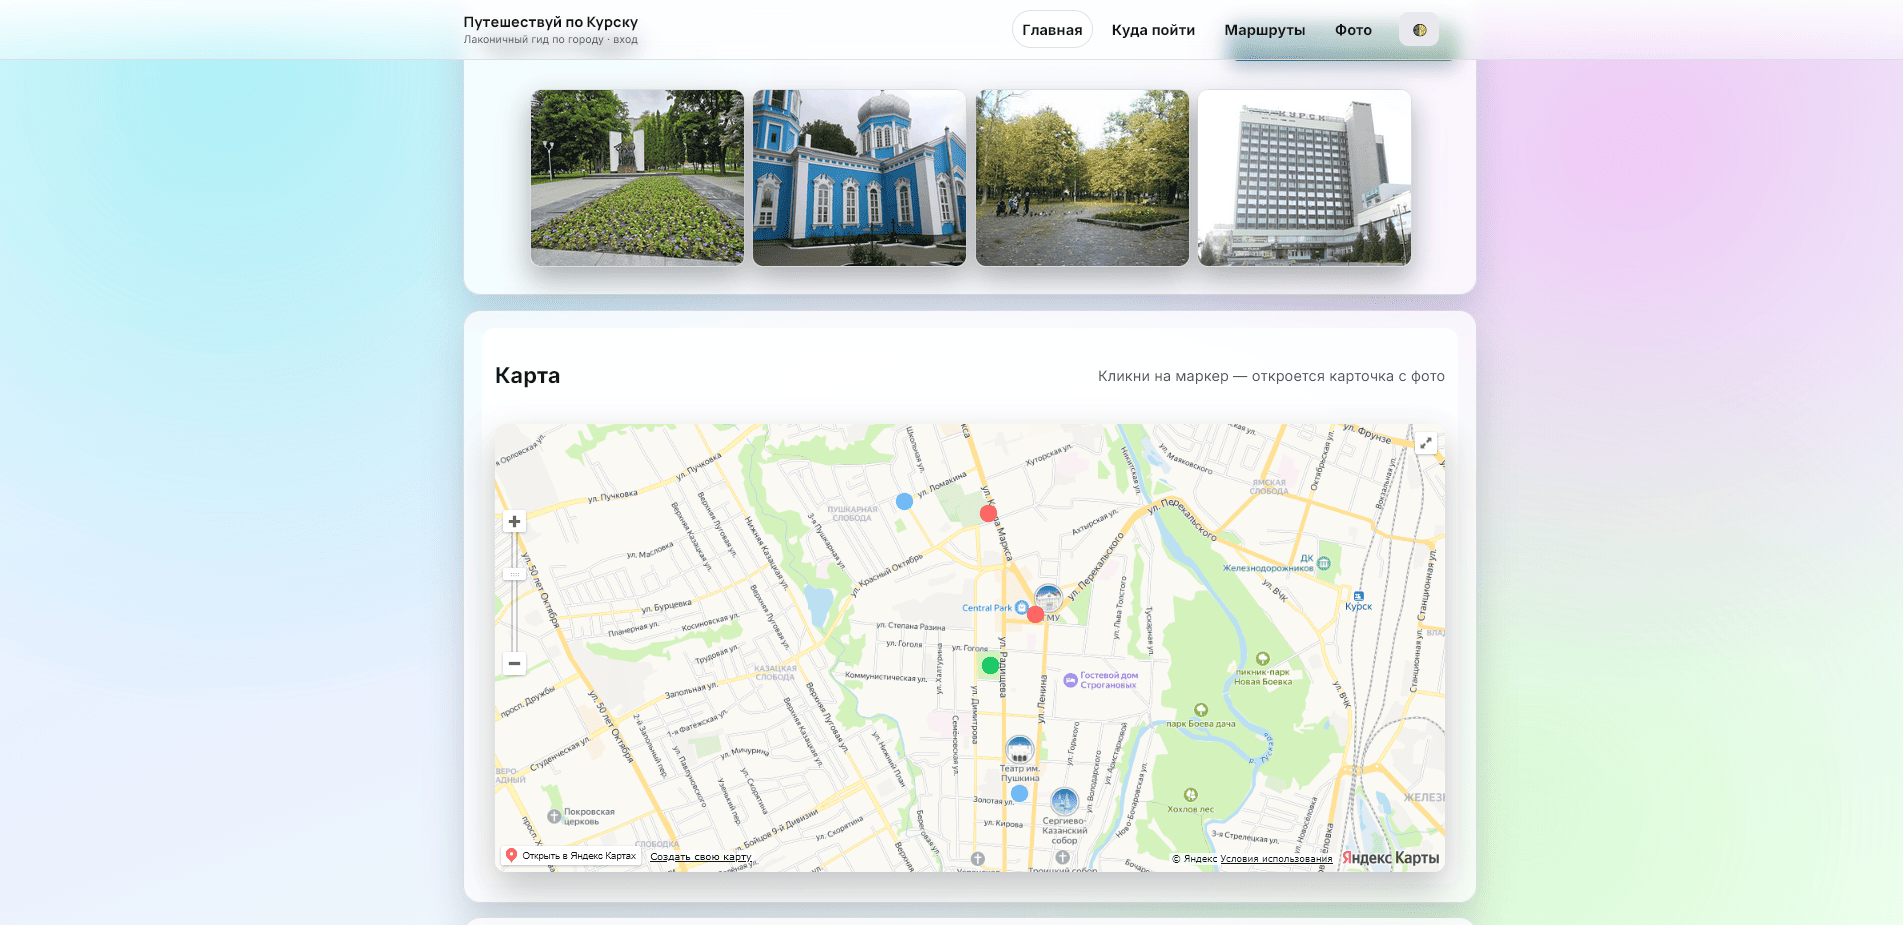
\includegraphics[width=0.9\linewidth]{images/ts-01}
	\caption{Главная страница с картой и маркерами (ТС-01)}
	\label{fig:ts-01}
\end{figure}

\subsubsection{TC-02. Фильтрация списка мест по категории}

\textbf{Предусловие:} открыта страница «Куда пойти» (\texttt{places.html}). В системе есть места разных категорий.

\textbf{Шаги:}
\begin{enumerate}
	\item В панели фильтров нажать кнопку с категорией «Парк».
	\item Проверить, что в списке карточек остались только места с категорией «парк».
	\item Нажать кнопку «Все».
	\item Убедиться, что снова отображаются все места.
\end{enumerate}

\textbf{Ожидаемый результат:} при выборе категории список карточек динамически обновляется без перезагрузки страницы. Фильтр применяется к текущему набору данных.

\textbf{Фактический результат:} пройден. Результат тестирования представ-
лен на рисунке~\ref{fig:ts-02}.

% Место для рисунка: страница places.html с активным фильтром

\begin{figure}[H]
	\centering
	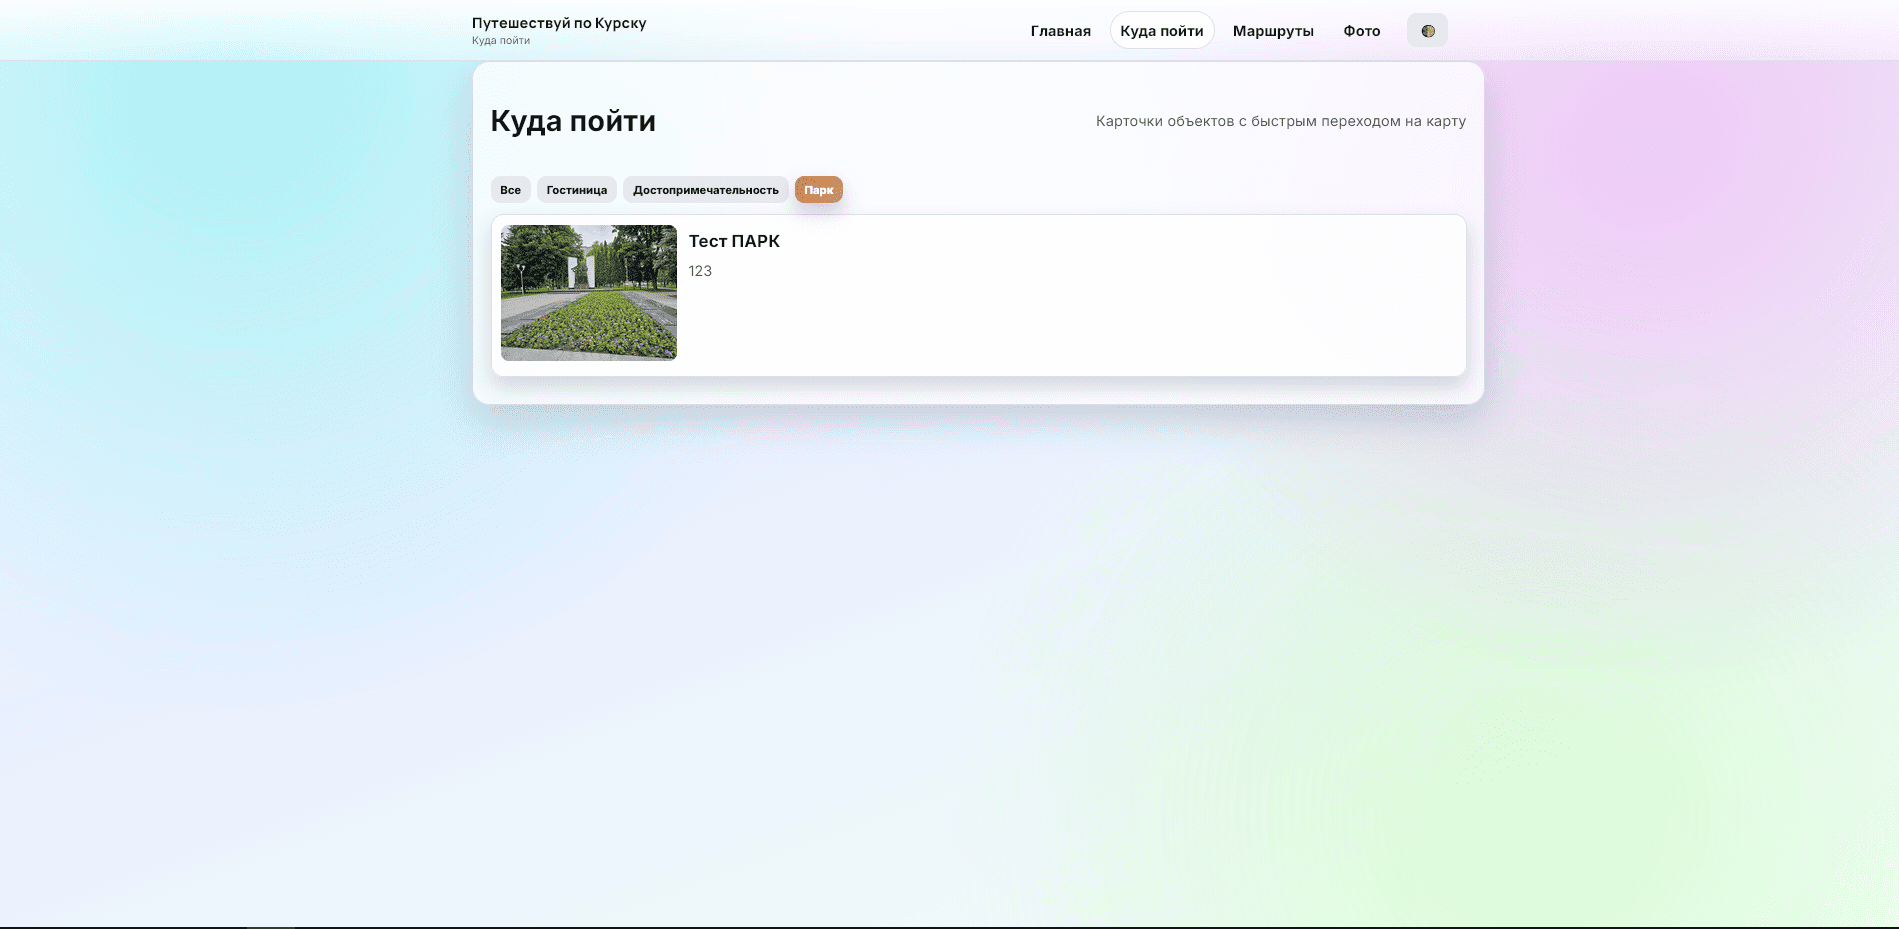
\includegraphics[width=0.9\linewidth]{images/ts-02}
	\caption{Страница «Куда пойти» с активным фильтром (ТС-02)}
	\label{fig:ts-02}
\end{figure}

\subsubsection{TC-03. Открытие карточки места и просмотр галереи}

\textbf{Предусловие:} открыта страница «Куда пойти» или главная страница с картой. Имеется место, у которого заполнены хотя бы одно изображение в галерее.

\textbf{Шаги:}
\begin{enumerate}
	\item Кликнуть по карточке места (или по маркеру на карте).
	\item В модальном окне проверить отображение названия, категории, описания, адреса, телефона, сайта.
	\item Пролистать до блока «Галерея» — увидеть миниатюры изображений.
\end{enumerate}

\textbf{Ожидаемый результат:} модальное окно содержит всю информацию об объекте. Галерея отображает до 10 изображений. Если галерея пуста, блок скрывается.

\textbf{Фактический результат:} пройден. Результат тестирования представ-
лен на рисунке~\ref{fig:ts-03}.

% Место для рисунка: модальное окно с карточкой места

\begin{figure}[H]
	\centering
	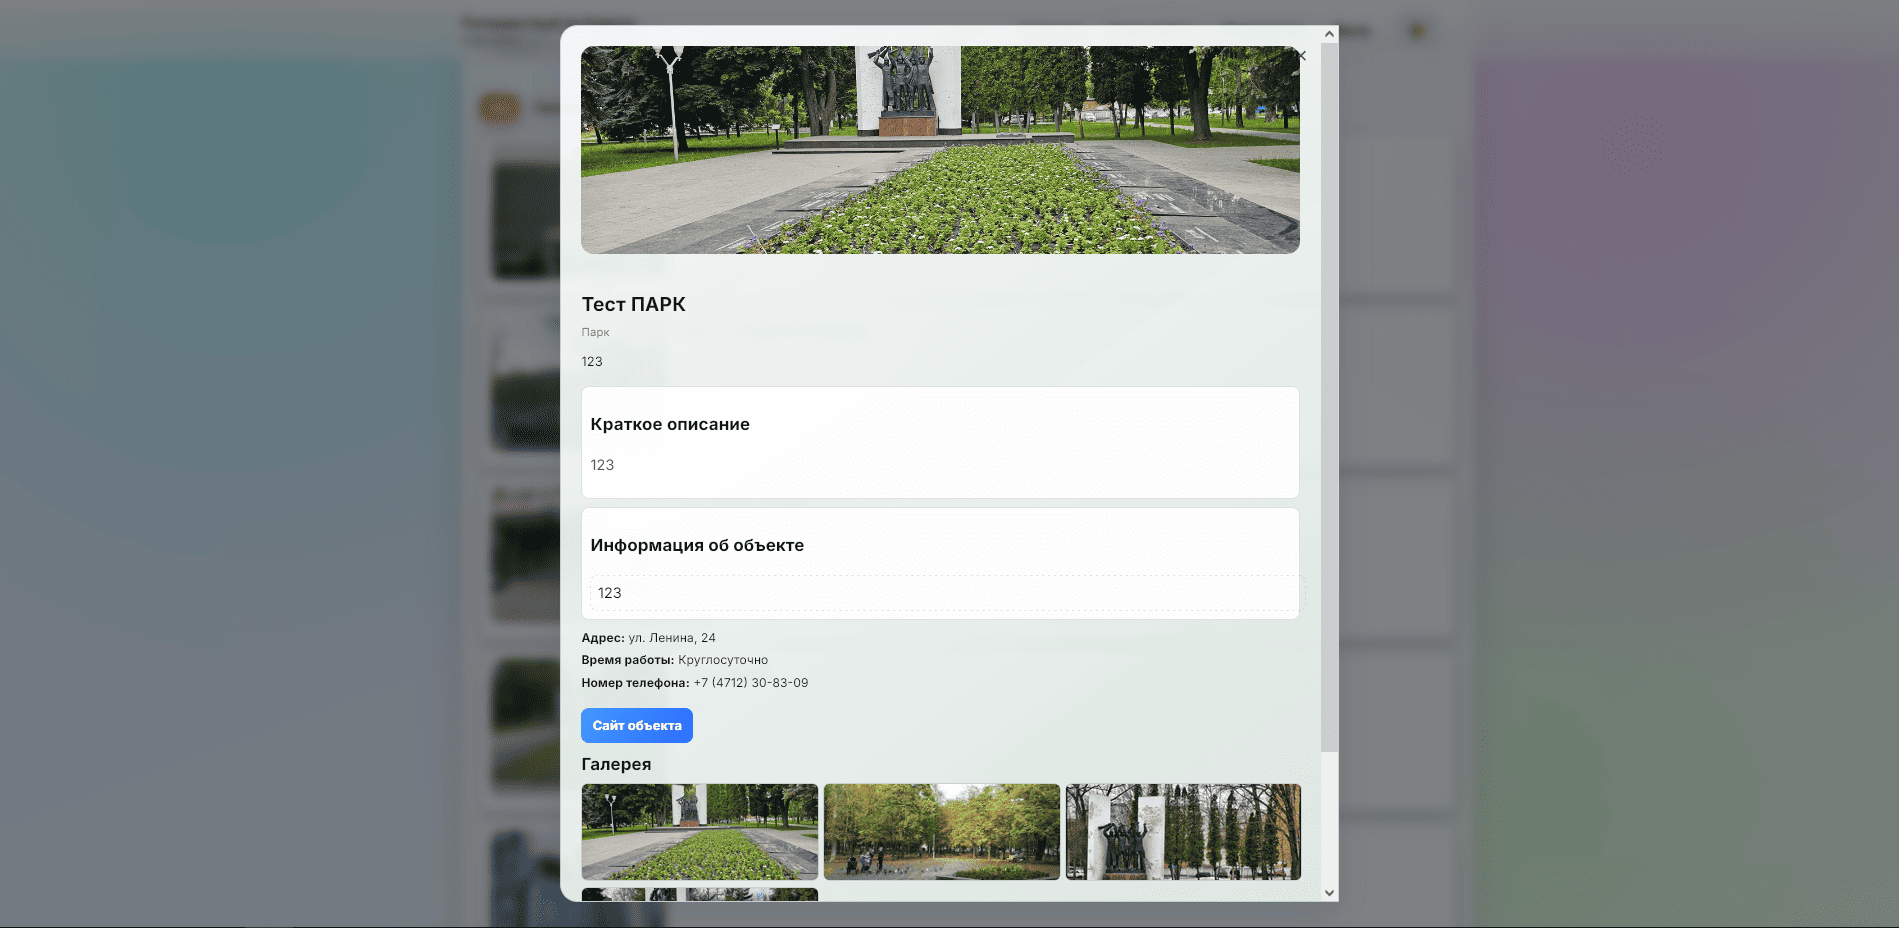
\includegraphics[width=0.9\linewidth]{images/ts-03}
	\caption{Модальное окно с карточкой места (ТС-03)}
	\label{fig:ts-03}
\end{figure}

\subsubsection{TC-04. Переход от карточки места к карте}

\textbf{Предусловие:} открыта карточка любого места (модальное окно).

\textbf{Шаги:}
\begin{enumerate}
	\item В карточке места найти кнопку «Показать на карте».
	\item Нажать на неё.
	\item Происходит переход на главную страницу (или страницу с картой), карта центрируется на выбранном месте, маркер подсвечивается.
\end{enumerate}

\textbf{Ожидаемый результат:} карта плавно перемещается к координатам места, открывается его краткая карточка (или всплывающая подсказка).

\textbf{Фактический результат:} пройден. Результат тестирования представ-
лен на рисунке~\ref{fig:ts-04}.

% Место для рисунка: карта с центрированием на месте

\begin{figure}[H]
	\centering
	
\includegraphics[width=0.9\linewidth]{images/ts-04}
	\caption{Краткая карточка объекта (ТС-04)}
	\label{fig:ts-04}
\end{figure}

\subsubsection{TC-05. Добавление нового места через админ-панель}

\textbf{Предусловие:} открыта страница администрирования.

\textbf{Шаги:}
\begin{enumerate}
	\item Заполнить форму: название «Тестовое место», выбрать категорию, указать широту и долготу, заполнить краткое описание, указать URL главного фото.
	\item По желанию добавить несколько URL в галерею (каждый с новой строки).
	\item Установить флаг «Опубликовать».
	\item Нажать «Сохранить объект».
	\item Проверить, что объект появился в таблице «Список объектов».
\end{enumerate}

\textbf{Ожидаемый результат:} объект добавляется в базу данных, отображается в админ-списке. На странице «Куда пойти» новое место видно в каталоге. На карте появляется соответствующий маркер.

\textbf{Фактический результат:} пройден. Результат тестирования представ-
лен на рисунке~\ref{fig:ts-05}.

% Место для рисунка: форма добавления места в админке

\begin{figure}[H]
	\centering
	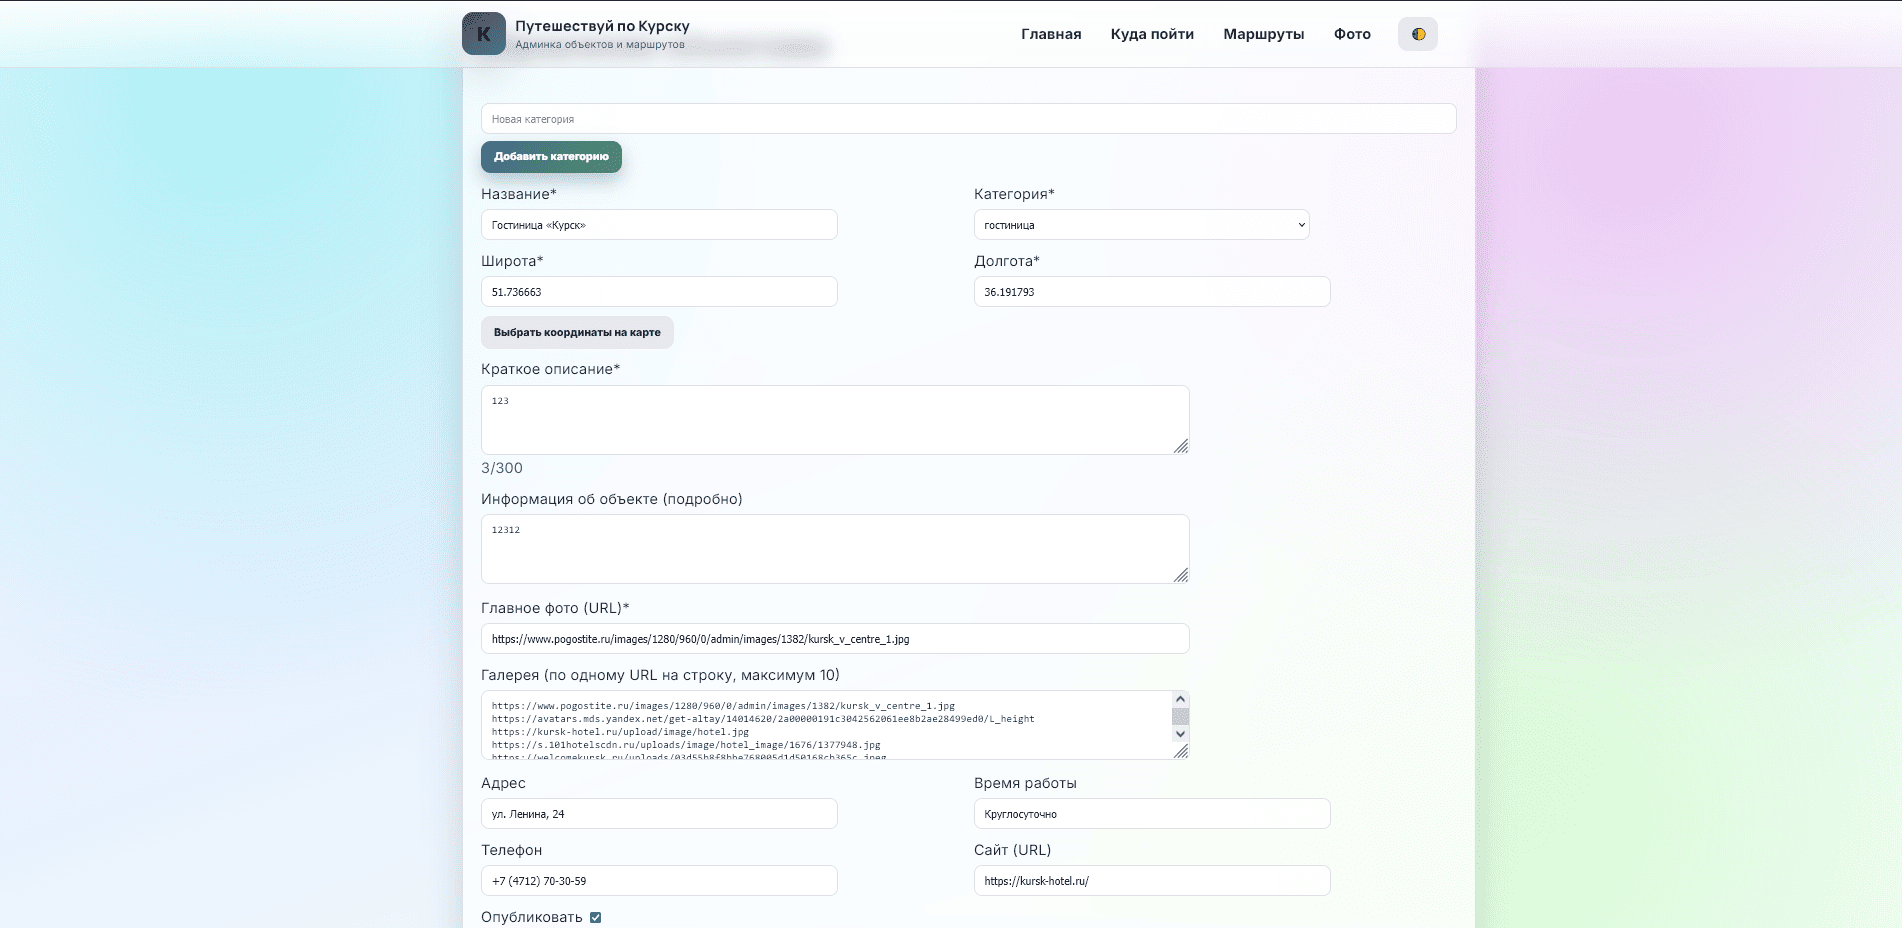
\includegraphics[width=0.9\linewidth]{images/ts-05}
	\caption{Форма добавления места (ТС-05)}
	\label{fig:ts-05}
\end{figure}

\subsubsection{TC-06. Редактирование существующего места}

\textbf{Предусловие:} в системе есть хотя бы одно место. Открыта админ-панель.

\textbf{Шаги:}
\begin{enumerate}
	\item В таблице «Список объектов» нажать кнопку «Редактировать» у выбранного места.
	\item Изменить название или описание.
	\item Нажать «Обновить объект».
\end{enumerate}

\textbf{Ожидаемый результат:} данные места обновляются в базе. На странице «Куда пойти» отображается актуальная информация.

\textbf{Фактический результат:} пройден. Результат тестирования представ-
лен на рисунке~\ref{fig:ts-06}.

% Место для рисунка: форма редактирования места

\begin{figure}[H]
	\centering
	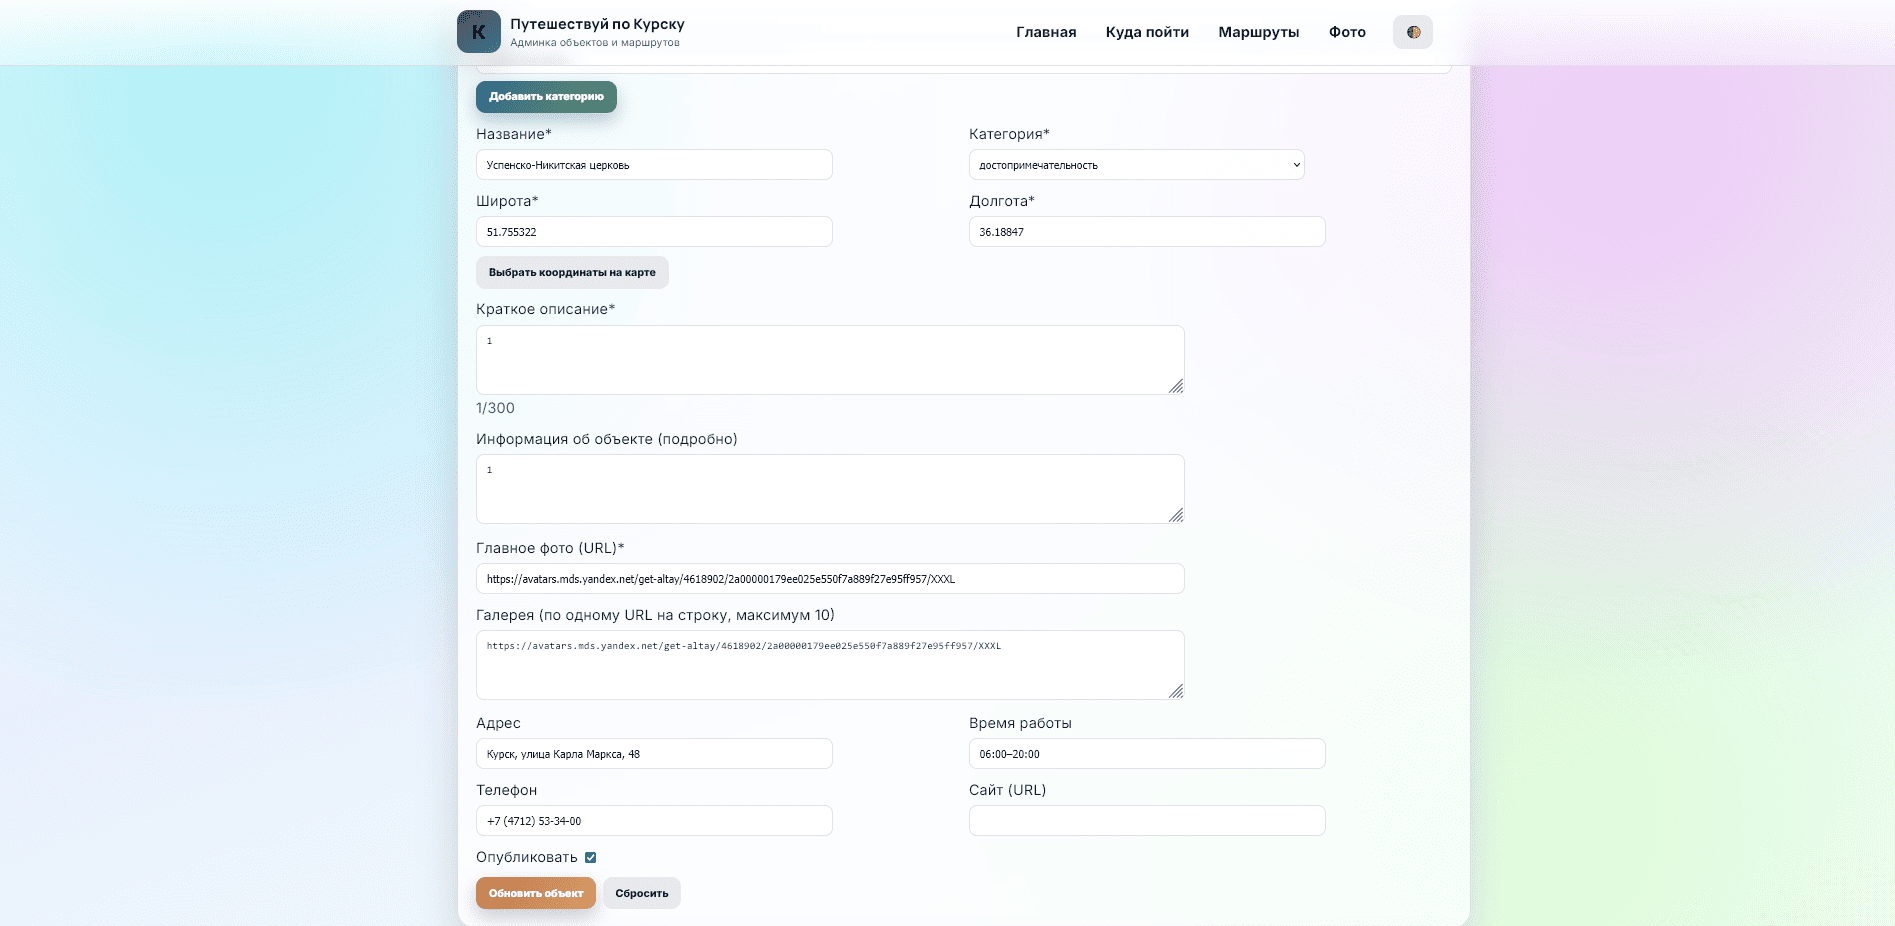
\includegraphics[width=0.9\linewidth]{images/ts-06}
	\caption{Форма редактирования места (ТС-06)}
	\label{fig:ts-06}
\end{figure}

\subsubsection{TC-07. Добавление новой категории}

\textbf{Предусловие:} открыта админ-панель.

\textbf{Шаги:}
\begin{enumerate}
	\item В поле «Новая категория» ввести, например, «Театр».
	\item Нажать кнопку «Добавить категорию».
	\item В выпадающем списке категорий (в форме объекта) появится новая категория.
\end{enumerate}

\textbf{Ожидаемый результат:} категория сохраняется в таблице \texttt{categories} и доступна для выбора при добавлении/редактировании мест.

\textbf{Фактический результат:} пройден. Результат тестирования представ-
лен на рисунке~\ref{fig:ts-07}.

% Место для рисунка: добавление категории

\begin{figure}[H]
	\centering
	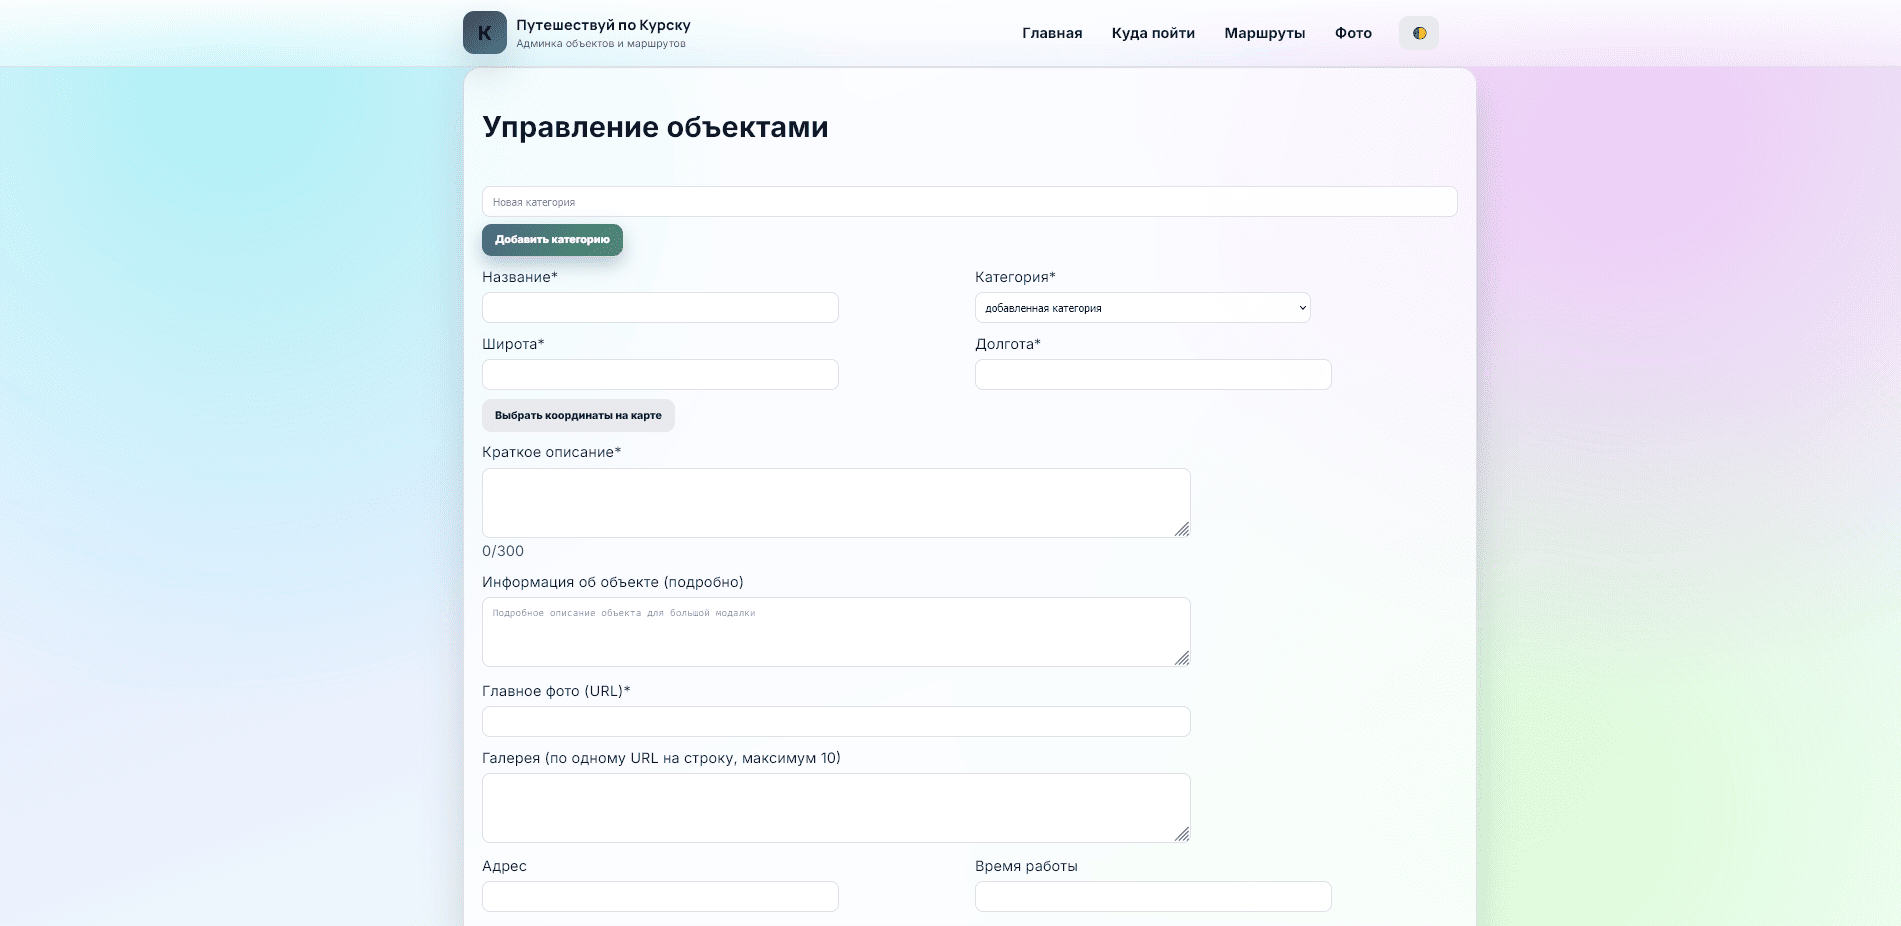
\includegraphics[width=0.9\linewidth]{images/ts-07}
	\caption{Добавленная категория (ТС-07)}
	\label{fig:ts-07}
\end{figure}

\subsubsection{TC-08. Создание маршрута (выбор точек, порядок)}

\textbf{Предусловие:} в системе существует минимум два места. Открыта админ-панель, раздел управления маршрутами.

\textbf{Шаги:}
\begin{enumerate}
	\item Заполнить название маршрута, краткое описание.
	\item В блоке «Точки маршрута» выбрать место из выпадающего списка и нажать «Добавить точку». Повторить для второго и третьего места.
	\item Изменить порядок точек кнопками «↑» и «↓».
	\item Установить флаг «Опубликовать».
	\item Нажать «Сохранить маршрут».
\end{enumerate}

\textbf{Ожидаемый результат:} маршрут сохраняется в БД. Точки сохраняются в таблице \texttt{route\_points} с правильными позициями. При попытке сохранить маршрут менее чем с двумя точками — ошибка валидации.

\textbf{Фактический результат:} пройден. Результат тестирования представ-
лен на рисунке~\ref{fig:ts-08}.

% Место для рисунка: форма создания маршрута

\begin{figure}[H]
	\centering
	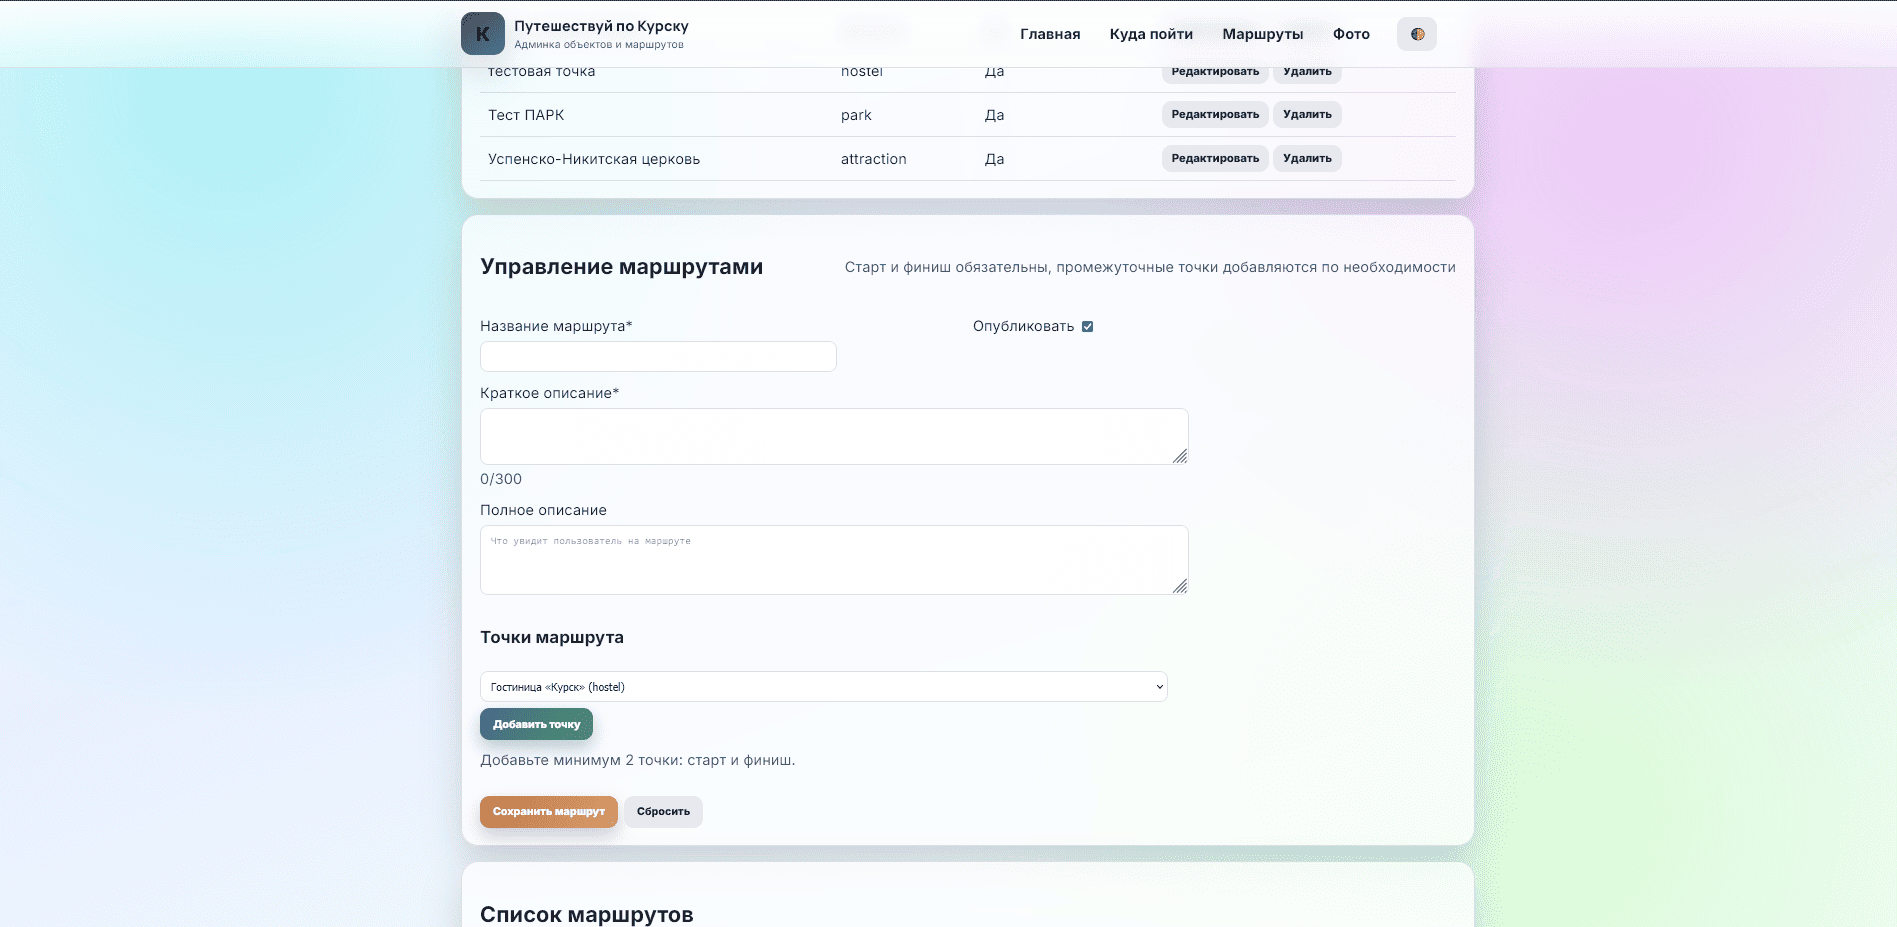
\includegraphics[width=0.9\linewidth]{images/ts-08}
	\caption{Форма создания маршрута (ТС-08)}
	\label{fig:ts-08}
\end{figure}

\subsubsection{TC-09. Редактирование маршрута}

\textbf{Предусловие:} в системе есть хотя бы один маршрут.

\textbf{Шаги:}
\begin{enumerate}
	\item В таблице «Список маршрутов» нажать «Редактировать».
	\item Изменить название, описание или состав точек.
	\item Сохранить изменения.
\end{enumerate}

\textbf{Ожидаемый результат:} маршрут обновляется в БД. При просмотре на странице «Маршруты» отображаются актуальные данные.

\textbf{Фактический результат:} пройден. Результат тестирования представ-
лен на рисунке~\ref{fig:ts-09}.

% Место для рисунка: редактирование маршрута

\begin{figure}[H]
	\centering
	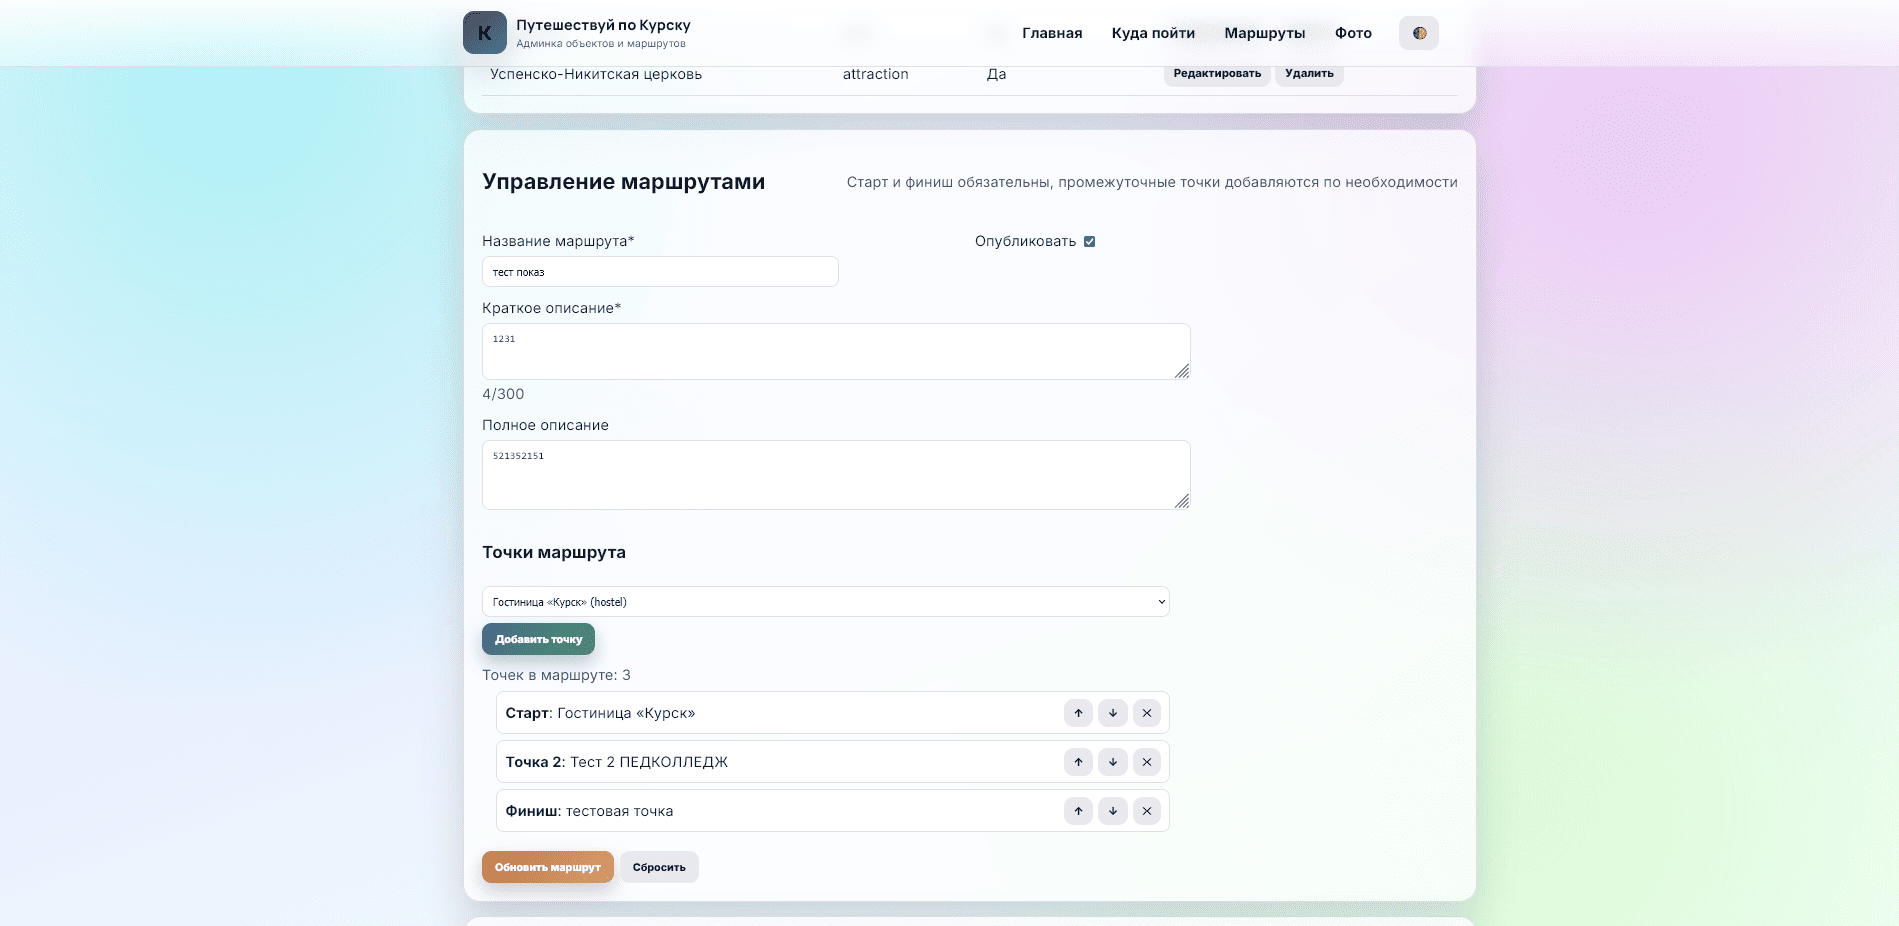
\includegraphics[width=0.9\linewidth]{images/ts-09}
	\caption{Форма редактирования маршрута (ТС-09)}
	\label{fig:ts-09}
\end{figure}

\subsubsection{TC-10. Просмотр маршрута на карте (пешеходная прокладка)}

\textbf{Предусловие:} опубликован маршрут с корректными координатами точек (минимум две).

\textbf{Шаги:}
\begin{enumerate}
	\item Перейти на страницу «Маршруты» (\texttt{routes.html}).
	\item Нажать кнопку «Открыть маршрут» на карточке любого маршрута.
	\item В модальном окне проверить описание и список точек.
	\item Дождаться загрузки карты в нижней части модального окна.
\end{enumerate}

\textbf{Ожидаемый результат:} на карте построена линия пешеходного маршрута с использованием \texttt{ymaps.multiRouter}. Отображаются старт, финиш и промежуточные точки.

\textbf{Фактический результат:} пройден. Результат тестирования представ-
лен на рисунке~\ref{fig:ts-10}.

% Место для рисунка: модальное окно с маршрутом на карте

\begin{figure}[H]
	\centering
	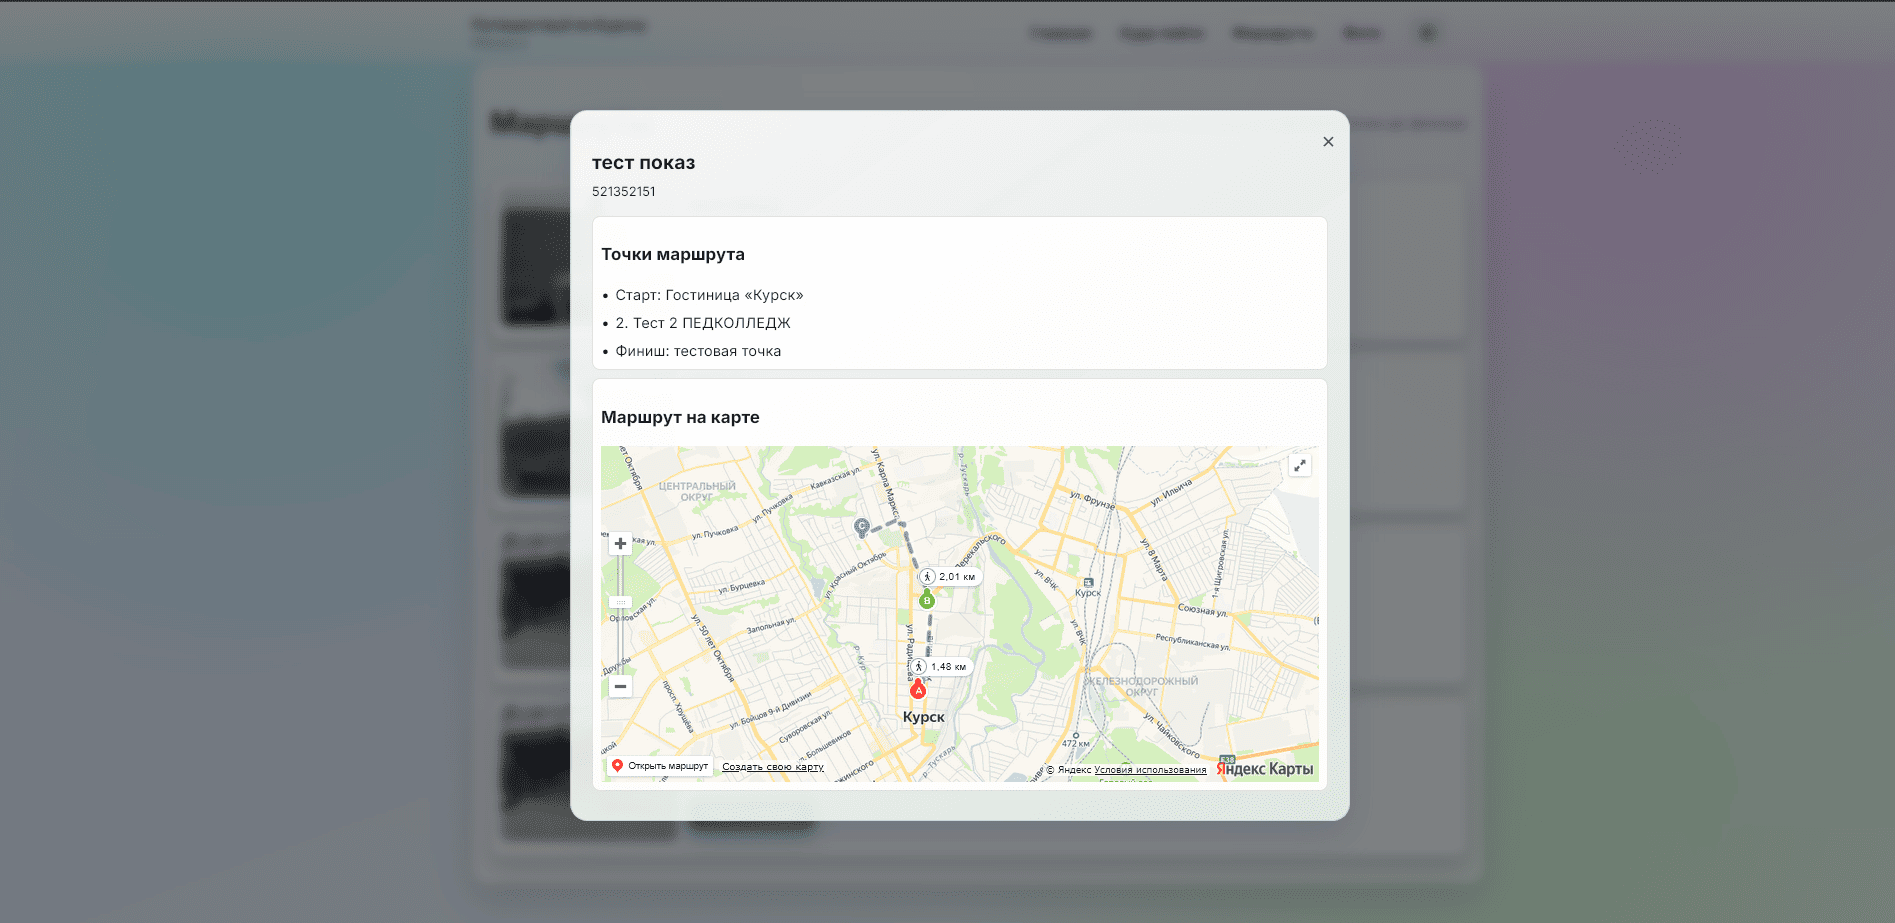
\includegraphics[width=0.9\linewidth]{images/ts-10}
	\caption{Модальное окно маршрута (ТС-10)}
	\label{fig:ts-10}
\end{figure}

\subsubsection{TC-11. Отображение фотогалереи всех мест}

\textbf{Предусловие:} в системе есть несколько мест с заполненными главными фото и галереями.

\textbf{Шаги:}
\begin{enumerate}
	\item Перейти на страницу «Фото».
	\item Просмотреть сетку изображений.
\end{enumerate}

\textbf{Ожидаемый результат:} сетка содержит все уникальные изображения (главные фото + галереи) из всех опубликованных мест. Порядок может быть случайным.

\textbf{Фактический результат:} пройден. Результат тестирования представ-
лен на рисунке~\ref{fig:ts-11}.

% Место для рисунка: страница photos.html

\begin{figure}[H]
	\centering
	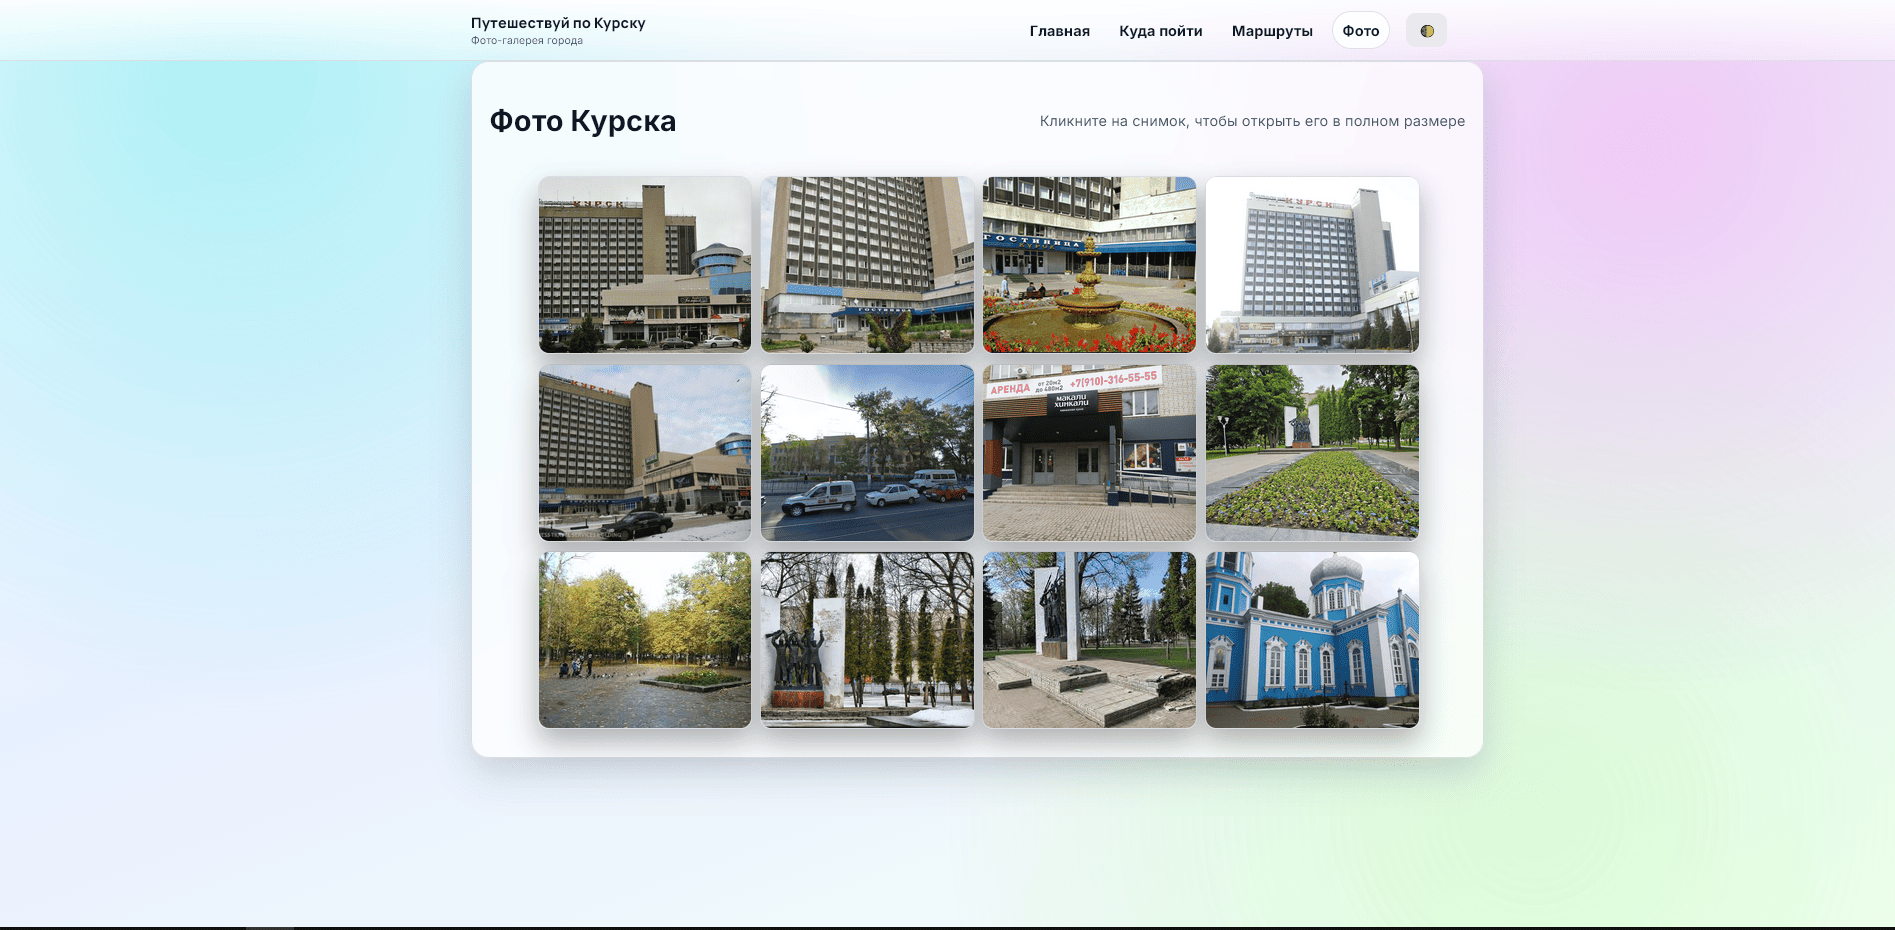
\includegraphics[width=0.9\linewidth]{images/ts-11}
	\caption{Страница «Фото» (ТС-11)}
	\label{fig:ts-11}
\end{figure}

\subsubsection{TC-12. Выбор координат объекта на карте в админке}

\textbf{Предусловие:} открыта форма добавления/редактирования места в админ-панели.

\textbf{Шаги:}
\begin{enumerate}
	\item Нажать кнопку «Выбрать координаты на карте».
	\item В открывшемся модальном окне дождаться загрузки карты.
	\item Кликнуть левой кнопкой мыши в любом месте карты.
	\item В диалоговом окне подтверждения нажать «OK».
\end{enumerate}

\textbf{Ожидаемый результат:} поля «Широта» и «Долгота» в форме автоматически заполняются выбранными координатами (6 знаков после запятой). Модальное окно закрывается.

\textbf{Фактический результат:} пройден. Результат тестирования представ-
лен на рисунке~\ref{fig:ts-14}.

% Место для рисунка: модальное окно выбора координат

\begin{figure}[H]
	\centering
	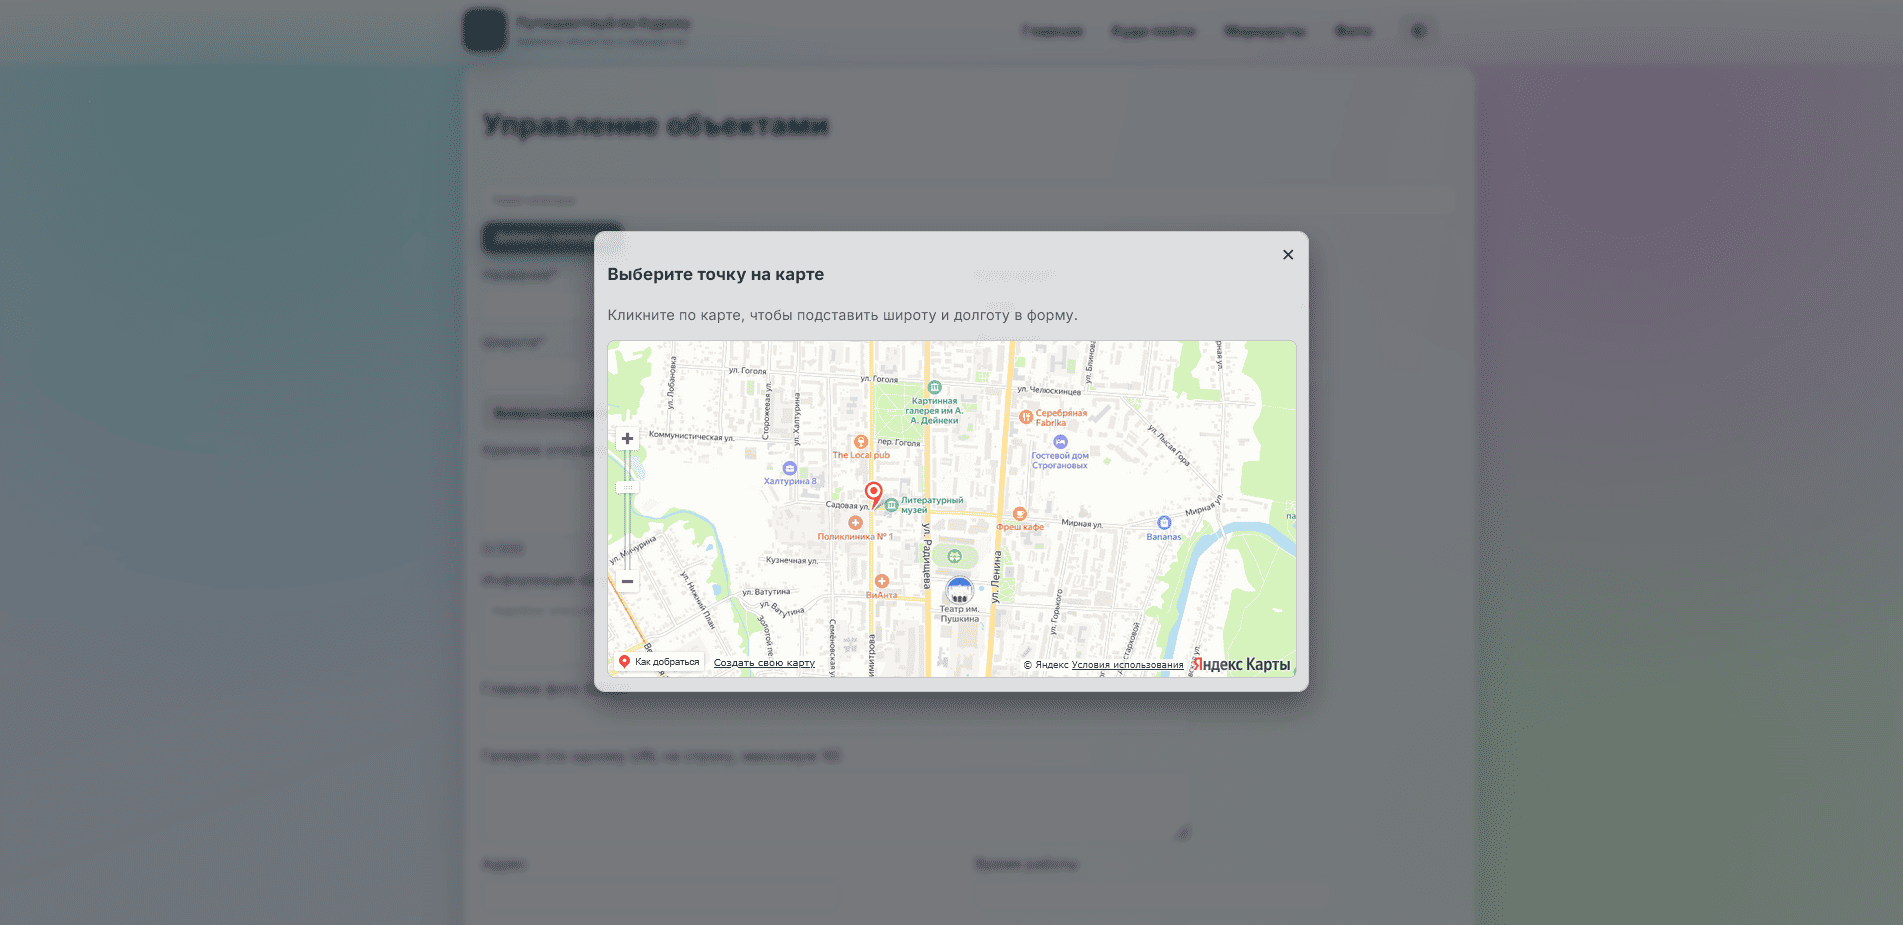
\includegraphics[width=0.9\linewidth]{images/ts-14}
	\caption{Модальное окно выбора координат (ТС-12)}
	\label{fig:ts-14}
\end{figure}

\subsubsection{Нефункциональное тестирование}

Проверены нефункциональные требования (разделы 2.6–2.8 ТЗ):

\begin{enumerate}
	\item Быстродействие: загрузка главной страницы с картой и 50 маркерами — не более 2 с. Фильтрация мест — мгновенно (< 100 мс). Сохранение места/маршрута — < 500 мс.
	\item Корректность логирования: ошибки API логируются в консоли сервера, клиенту возвращается JSON с полем \texttt{error}.
	\item Совместимость с браузерами: тестирование в Chrome, Firefox, Yandex Browser, Edge — все функции работают корректно.
	\item Надёжность: при разрыве соединения с БД сервер возвращает HTTP 500. Транзакционное сохранение маршрута гарантирует целостность.
\end{enumerate}

Все нефункциональные требования выполнены.

\subsubsection{Вывод по результатам тестирования}

В ходе системного тестирования успешно проверены все функциональные и нефункциональные требования. Веб-приложение работает стабильно, интерфейс интуитивно понятен, все сценарии использования выполняются корректно. Система готова к эксплуатации.
   \section*{ЗАКЛЮЧЕНИЕ}
\addcontentsline{toc}{section}{ЗАКЛЮЧЕНИЕ}
В процессе выполнения работы была создана программно-информационная система «Цифровая платформа Курский край» — интерактивный веб-гид по городу Курску. Были реализованы функции для пользователей и администратора.

Пользователи имеют возможность просматривать список мест с фильтрацией по категориям (парки, музеи, кафе, отели и т.д.), открывать подробные карточки объектов с описанием, контактами и галереей, а также просматривать маршруты и видеть их визуализацию на карте. Администратор может добавлять, редактировать и удалять объекты и маршруты, а также создавать новые категории.

Основные результаты работы:

\begin{enumerate}
	\item Проведён анализ предметной области. Выявлены ключевые сущности (категории, места, маршруты, точки маршрута) и обоснована необходимость автоматизации.
	\item Разработана концептуальная модель веб-сайта. Построена ER-модель базы данных. Определены функциональные и нефункциональные требования к системе.
	\item Осуществлено проектирование веб-сайта. Разработана архитектура клиент-сервер. Спроектирован пользовательский интерфейс.
	\item Реализован и протестирован веб-сайт. Проведено модульное и системное тестирование.
\end{enumerate}

Все требования, объявленные в техническом задании, были полностью реализованы, все задачи, поставленные в начале разработки проекта, также решены.

Сайт находится в публичном доступе, поскольку опубликован в сети Интернет.  

}\fi
\addcontentsline{toc}{section}{СПИСОК ИСПОЛЬЗОВАННЫХ ИСТОЧНИКОВ}

\begin{thebibliography}{99}
	
	\bibitem{gost1} ГОСТ 19.102–77. Единая система программной документации. Стадии разработки : межгосударственный стандарт : издание официальное : утвержден Постановлением Государственного комитета стандартов Совета Министров СССР от 20 декабря 1977 г. № 2851 : дата введения 1980-01-01. --- Москва : Стандартинформ, 2010. --- Текст : непосредственный.
	
	\bibitem{gost2} ГОСТ 34.601–90. Информационная технология. Комплекс стандартов на автоматизированные системы. Автоматизированные системы. Стадии создания : межгосударственный стандарт : издание официальное : утвержден и введен в действие Постановлением Государственного комитета СССР по управлению качеством продукции и стандартам от 29 декабря 1990 г. № 3469 : дата введения 1992-01-01. --- Москва : Стандартинформ, 2009. --- Текст : непосредственный.
	
	\bibitem{gost3} ГОСТ Р 7.0.5–2008. Система стандартов по информации, библиотечному и издательскому делу. Библиографическая ссылка. Общие требования и правила составления : национальный стандарт Российской Федерации : издание официальное : утвержден и введен в действие Приказом Федерального агентства по техническому регулированию и метрологии от 28 апреля 2008 г. № 95-ст : дата введения 2009-01-01. --- Москва : Стандартинформ, 2008. --- Текст : непосредственный.
	
	\bibitem{gost4} ГОСТ Р ИСО/МЭК 25010–2015. Информационные технологии. Системная и программная инженерия. Требования и оценка качества систем и
	программного обеспечения (SQuaRE). Модели качества систем и программных продуктов : национальный стандарт Российской Федерации : издание
	официальное : утвержден и введен в действие Приказом Федерального агент-
	ства по техническому регулированию и метрологии от 29 мая 2015 г. № 442-
	ст : дата введения 2016-06-01. --- Москва : Стандартинформ, 2015. --- Текст :	непосредственный.
	
	\bibitem{gost5} ГОСТ Р ИСО 21500–2023. Управление проектами, программами и портфелями проектов. Контекст и основные понятия : национальный стандарт Российской Федерации : издание официальное : утвержден и введен в действие Приказом Федерального агентства по техническому регулированию и метрологии от 30 октября 2023 г. № 1296-ст : дата введения 2024-06-01. --- Москва : Российский институт стандартизации, 2023. --- Текст : непосредственный.
	
	\bibitem{gost5} ГОСТ Р 54869–2011. Проектный менеджмент. Требования к управлению проектом : национальный стандарт Российской Федерации : издание официальное : утвержден и введен в действие Приказом Федерального агентства по техническому регулированию и метрологии от 22 декабря 2011 г.
	№ 1582-ст : дата введения 2012-09-01. --- Москва : Стандартинформ, 2012. --- Текст : непосредственный.
	
	\bibitem{postgresql-admin} Бек, К. Экстремальное программирование. Разработка через тестирование / К. Бек ; перевод с английского. --- Санкт-Петербург : Питер, 2017. --- 224 с. --- (Библиотека программиста). --- ISBN 978-5-496-02570-6. --- Текст : непосредственный.
	
	\bibitem{database} Буч, Г. Язык UML. Руководство пользователя / Г. Буч, Дж. Рамбо, И. Якобсон ; перевод с английского. --- 2-е изд. --- Москва : ДМК Пресс, 2015. --- 496 с. --- ISBN 978-5-94074-644-7. --- Текст : непосредственный.
	
	\bibitem{sql-antipatterns} Буч, Г. Объектно-ориентированный анализ и проектирование с примерами приложений / Г. Буч, Р. А. Максимчук, М. У. Энгл [и др.] ; перевод с английского. --- 3-е изд. --- Москва : ООО «И.Д. Вильямс», 2010. --- 720 с. --- ISBN 978-5-8459-1401-9. --- Текст : непосредственный.
	
	\bibitem{htmlcss} Гамма, Э. Паттерны объектно-ориентированного проектирования / Э. Гамма, Р. Хелм, Р. Джонсон, Дж. Влиссидес ; перевод с английского. --- Санкт-Петербург : Питер, 2020. – 448 с. --- (Библиотека программиста). --- ISBN 978-5-4461-1595-2. --- Текст : непосредственный.
	
	\bibitem{html5} Дейт, К. Дж. Введение в системы баз данных / К. Дж. Дейт ; перевод с английского. --- 8-е изд. --- Москва : ООО «И.Д. Вильямс», 2005. --- 1328 с. --- ISBN 5-8459-0788-8. --- Текст : непосредственный.
	
	\bibitem{css} Лоре, А. Проектирование веб-API / А. Лоре ; перевод с английского. --- Москва : ДМК Пресс, 2020. --- 440 с. --- ISBN 978-5-97060-861-6. --- Текст : непосредственный
	
	\bibitem{css-big-book} Управление проектами : учебное пособие / И. И. Мазур, В. Д. Шапиро, Н. Г. Ольдерогге, А. В. Полковников ; под общей редакцией И. И. Мазура и В. Д. Шапиро. --- 10-е изд., стер. --- Москва : Омега-Л, 2014. --- 960 с. --- ISBN 978-5-370-02800-7. --- Текст : непосредственный
	
	\bibitem{web-design} Орлов, С. А. Программная инженерия. Технологии разработки программного обеспечения : учебник для вузов / С. А. Орлов. --- 5-е изд., обнов. и доп. --- Санкт-Петербург : Питер, 2020. – 640 с. --- (Учебник для вузов. Стандарт третьего поколения). --- ISBN 978-5-4461-1348-4. --- Текст : непосредственный.
	
	\bibitem{dont-make-me-think} Робсон, Э. Изучаем HTML и CSS / Э. Робсон, Э. Фримен ; перевод с английского. --- 2-е изд. --- Санкт-Петербург : Питер, 2014. --- 720 с. --- (Head First O’Reilly). --- ISBN 978-5-496-00653-8. --- Текст : непосредственный.
	
	\bibitem{uml} Фаулер, М. UML. Основы : краткое руководство по стандартному
	языку объектного моделирования / М. Фаулер ; перевод с английского. --- 3-е изд. --- Санкт-Петербург : Символ-Плюс, 2013. --- 192 с. --- ISBN 5-93286-060-X. --- Текст : непосредственный
	
	\bibitem{softwareengineering} Фаулер, М. Шаблоны корпоративных приложений / М. Фаулер, Д. Райс, М. Фоммел [и др.] ; перевод с английского. --- Москва : ООО «И.Д. Вильямс», 2018. – 544 с. – ISBN 978-5-8459-1611-2. --- Текст : непосредственный.
	
	\bibitem{pressman} Флэнаган, Д. JavaScript. Полное руководство / Д. Флэнаган ; перевод с английского. --- 7-е изд. --- Москва : ООО «Диалектика», 2021. --- 720 с. – ISBN 978-5-907203-79-2. --- Текст : непосредственный.
	
	\bibitem{clean-code} Якобсон, А. Унифицированный процесс разработки программного обеспечения / А. Якобсон, Г. Буч, Дж. Рамбо ; перевод с английского. --- Санкт-Петербург : Питер, 2002. --- 496 с. --- (Классика computer science). --- ISBN 5-318-00358-3. --- Текст : непосредственный.
	
	\bibitem{refactoring} Руководство к своду знаний по управлению проектами (Руководство PMBOK). Шестое издание + Agile : практическое руководство / Project Management Institute ; перевод с английского. --- Москва : Олимп-Бизнес, 2022. --- 974 с. --- ISBN 978-5-9693-0402-4. --- Текст : непосредственный.
	
	\bibitem{http-definitive} Шор, А. М. Сравнительный анализ подходов в разработке API веб-приложений / А. М. Шор. // StudNet. --- 2020. --- № 9. --- URL: \url{https://cyberleninka.ru/article/n/sravnitelnyy-analiz-podhodov-v-razrabotke-api-veb-prilozheniy} (дата обращения: 10.05.2026).
	
	\bibitem{rest} Филдинг, Р. Архитектурные стили и проектирование сетевых программных архитектур / Р. Филдинг. --- 2000. --- URL: \url{https://www.ics.uci.edu/~fielding/pubs/dissertation/top.htm} (дата обращения: 21.01.2026).
	
	\bibitem{gost-34-201} ГОСТ 34.201-2020. Информационные технологии. Комплекс стандартов на автоматизированные системы. Виды, комплектность и обозначение документов при создании автоматизированных систем. --- Москва : Стандартинформ, 2020. --- Текст : непосредственный.
	
	\bibitem{gost-34-602} ГОСТ 34.602-2020. Информационные технологии. Комплекс стандартов на автоматизированные системы. Техническое задание на создание автоматизированной системы. --- Москва : Стандартинформ, 2020. --- Текст : непосредственный.
	
	\bibitem{gost-19-701} ГОСТ 19.701-90. Единая система программной документации. Схемы алгоритмов, программ, данных и систем. --- Москва : Стандартинформ, 2010. --- Текст : непосредственный.
	
	\bibitem{iso-sql} Сафонова, А. А. Информационные системы управления проек-
	тами / А. А. Сафонова, О. Н. Куксачева. // Формула менеджмента. ---
	2020. --- № 1. --- URL: \url{https://cyberleninka.ru/article/n/informatsionnye-sistemy-
	upravleniya-proektami} (дата обращения: 10.04.2026).
	
	\bibitem{mdn-html} HTML: HyperText Markup Language // MDN Web Docs : [сайт]. --- URL: \url{https://developer.mozilla.org/docs/Web/HTML} (дата обращения: 10.01.2026).
	
	\bibitem{mdn-css} CSS: Cascading Style Sheets // MDN Web Docs : [сайт]. --- URL: \url{https://developer.mozilla.org/docs/Web/CSS} (дата обращения: 10.01.2026).
	
	\bibitem{mdn-js} JavaScript // MDN Web Docs : [сайт]. --- URL: \url{https://developer.mozilla.org/docs/Web/JavaScript} (дата обращения: 14.01.2026).
	
	\bibitem{mdn-dom} Document Object Model (DOM) // MDN Web Docs : [сайт]. --- URL: \url{https://developer.mozilla.org/docs/Web/API/Document_Object_Model} (дата обращения: 15.01.2026).
	
	\bibitem{mdn-fetch} Fetch API // MDN Web Docs : [сайт]. --- URL: \url{https://developer.mozilla.org/docs/Web/API/Fetch_API} (дата обращения: 02.02.2026).
	
	\bibitem{mdn-http} HTTP // MDN Web Docs : [сайт]. --- URL: \url{https://developer.mozilla.org/docs/Web/HTTP} (дата обращения: 04.02.2026).
	
	\bibitem{mdn-json} JSON // MDN Web Docs : [сайт]. --- URL: \url{https://developer.mozilla.org/docs/Glossary/JSON} (дата обращения: 11.02.2026).
	
	\bibitem{node-docs} Node.js Documentation : [сайт]. --- URL: \url{https://nodejs.org/docs/latest/api/} (дата обращения: 11.05.2026).
	
	\bibitem{npm-docs} npm Docs : [сайт]. --- URL: \url{https://docs.npmjs.com/} (дата обращения: 20.02.2026).
	
	\bibitem{express-docs} Express 4.x API Reference : [сайт]. --- URL: \url{https://expressjs.com/en/4x/api.html} (дата обращения: 01.03.2026).
	
	\bibitem{pg-docs} node-postgres Documentation. --- URL: \url{https://node-postgres.com/} (дата обращения: 05.03.2026).
	
	\bibitem{postgres-docs} PostgreSQL Documentation : [сайт]. --- URL: \url{https://www.postgresql.org/docs/} (дата обращения: 10.03.2026).
	
	\bibitem{postgres-json} PostgreSQL Documentation. JSON Types : [сайт]. --- URL: \url{https://www.postgresql.org/docs/current/datatype-json.html} (дата обращения: 11.03.2026).
	
	\bibitem{yandex-maps} JavaScript API Яндекс Карт. Руководство разработчика : [сайт]. --- URL: \url{https://yandex.ru/dev/maps/jsapi/} (дата обращения: 20.03.2026).
	
	\bibitem{html-standard} HTML Standard // WHATWG : [сайт]. --- URL: \url{https://html.spec.whatwg.org/docs} (дата обращения: 25.03.2026).
	
	\bibitem{css-w3c} CSS Snapshot // W3C : [сайт]. --- URL: \url{https://www.w3.org/TR/CSS/} (дата обращения: 02.04.2026).
	
	\bibitem{ecma262} ECMAScript Language Specification // ECMA International : [сайт]. --- URL: \url{https://tc39.es/ecma262/} (дата обращения: 12.04.2026).
	
	\bibitem{rfc-http} Fielding, R. HTTP Semantics. RFC 9110 / R. Fielding, M. Nottingham, J. Reschke : [сайт]. --- URL: \url{https://www.rfc-editor.org/rfc/rfc9110} (дата обращения: 12.02.2026).
	
	\bibitem{rfc-uri} Berners-Lee, T. Uniform Resource Identifier (URI): Generic Syntax. RFC 3986 / T. Berners-Lee, R. Fielding, L. Masinter : [сайт]. --- URL: \url{https://www.rfc-editor.org/rfc/rfc3986} (дата обращения: 16.04.2026).
	
	\bibitem{rfc-json} Bray, T. The JavaScript Object Notation (JSON) Data Interchange Format. RFC 8259 / T. Bray : [сайт]. --- URL: \url{https://www.rfc-editor.org/rfc/rfc8259} (дата обращения: 13.03.2026).
	
	\bibitem{owasp-top-ten} OWASP Top Ten Web Application Security Risks // OWASP : [сайт]. --- URL: \url{https://owasp.org/www-project-top-ten/} (дата обращения: 11.05.2026).
	
	\bibitem{web-accessibility} Web Content Accessibility Guidelines (WCAG) 2.2 // W3C : [сайт]. --- URL: \url{https://www.w3.org/TR/WCAG22/} (дата обращения: 11.05.2026).
	
	\bibitem{git-docs} Git Documentation. --- URL: \url{https://git-scm.com/} (дата обращения: 09.01.2026).
	
	\bibitem{vscode-docs} Visual Studio Code Documentation. --- URL: \url{https://code.visualstudio.com/} (дата обращения: 09.01.2026).
	
\end{thebibliography}
\ifВКР{\appendix{Представление графического материала}

Графический материал, выполненный на отдельных листах,
изображен на рисунках А.1--А.\arabic{числоПлакатов}.
\setcounter{числоПлакатов}{0}

\renewcommand{\thefigure}{А.\arabic{figure}} % шаблон номера для плакатов

\begin{landscape}

\begin{плакат}
    
\includegraphics[width=0.82\linewidth]{main.eps}
    \заголовок{Сведения о ВКРБ}
    \label{pl1:image}      
\end{плакат}

\begin{плакат}
    
\includegraphics[width=0.82\linewidth]{goal.eps}
    \заголовок{Цель и задачи разработки}
    \label{pl2:image}      
\end{плакат}

\begin{плакат}
    
\includegraphics[width=0.82\linewidth]{komponenti.eps}
    \заголовок{Диаграмма компонентов ситемы}
    \label{pl3:image}      
\end{плакат}

\begin{плакат}
    
\includegraphics[width=0.82\linewidth]{ispolzovanie.eps}
    \заголовок{Диаграмма прецедентов}
    \label{pl4:image}      
\end{плакат}

\begin{плакат}
	
\includegraphics[width=0.82\linewidth]{routes.eps}
	\заголовок{Диаграмма последовательности просмотра маршрута}
	\label{pl5:image}      
\end{плакат}

\begin{плакат}
	
\includegraphics[width=0.82\linewidth]{object.eps}
	\заголовок{Диаграмма последовательности добавления объекта}
	\label{pl6:image}      
\end{плакат}

\begin{плакат}
	
\includegraphics[width=0.82\linewidth]{conclusion.eps}
	\заголовок{Заключение}
	\label{pl7:image}      
\end{плакат}

\end{landscape}
}\fi
\ifПрактика{}\else{\appendix{Фрагменты исходного кода программы}

app.js
\lstinputlisting[language=C, frame=none]{app.js}

admin-page.js
\lstinputlisting[language=C, frame=none]{admin-page.js}

\ifВКР{
\newpage
\addcontentsline{toc}{section}{На отдельных листах (CD-RW в прикрепленном конверте)}
\noindent
\begin{tabular}{p{5.8cm}C{4.8cm}C{4.8cm}}
   Автор ВКР & \lhrulefill{\fill} & \fillcenter\Автор \\
            \setarstrut{\footnotesize}
           & \footnotesize{(подпись, дата)} & \\
            \restorearstrut
   Руководитель ВКР & \lhrulefill{\fill} & \fillcenter\Руководитель \\
            \setarstrut{\footnotesize}
           & \footnotesize{(подпись, дата)} & \\
            \restorearstrut
   Нормоконтроль & \lhrulefill{\fill} & \fillcenter\Нормоконтроль \\
            \setarstrut{\footnotesize}
           & \footnotesize{(подпись, дата)} & \\
            \restorearstrut
\end{tabular}
\vskip 2cm
\begin{center}
\textbf{Место для диска}
\end{center}
}\fi
}\fi
\end{document}
